\chapter[Towards a Computational Theory of \textsl{Rasa}]{Towards a Computational Theory of \textsl{Rasa}$^{*}$}\label{chapter\thechapter:begin}
\footnotetext[1]{pp.~\pageref{chapter\thechapter:begin}--\pageref{chapter-3:end}. In: Kannan, K S (Ed.) (2018) {\sl Western Indology On Rasa – A Pūrvapakṣa}. Chennai: Infinity Foundation India.}

\begin{center}
{\bf A framework for \textsl{pratibhā} and \textsl{kalā} in general}
\index{pratibha@\textsl{pratibhā}}
%{\bf (commonality across \textsl{kalā}-s)}
\end{center}
\index{kala@\textsl{kalā}}

\Authorline{K. Gopinath}
\lhead[\small\thepage\quad K. Gopinath]{}

\section*{Abstract}

Prof. Sheldon Pollock opines that Indian thinkers have neither attempted a robust theory for creativity nor did they have theory across \hbox{\textsl{kalā}-s}. We arque here against this opinion by sketching a computationally inspired theory of \textsl{rasa}\index{rasa@\textsl{rasa}} (a work in progress), and attempt to uncover Indic insights over the ages in support of the theory. Finally, we illustrate it with examples from certain art forms.

\bigskip
\noindent
{\large Contents}

{\renewcommand{\arraystretch}{1.15}
\begin{longtable}[l]{l@{\;\;\;}l@{\;\;\;}p{8cm}}
1 & \multicolumn{2}{@{}l}{Introduction}\\
  & 1.1 & An Initial Riposte\\
  & 1.2 & Outline of the Paper\\
  & 1.3 & Commonalities across painting and other arts as per Citra-sūtra\\
2 & \multicolumn{2}{@{}l}{A Brief Introduction to Rasa}\\
3 & \multicolumn{2}{@{}l}{A High Level Theory for Rasa}\\
  & 3.1 & Current theories of mind related to Rasa and synergistic models\\
4 & \multicolumn{2}{@{}l}{Outline of a contemporaneous Indic theory for Rasa}\\
  & 4.1 & The “atomic units” in the various art forms and higher-level structures\\
  & 4.2 & A computer systems model for communication across multiple roles and multiple persons\\
  & 4.3 & Rasa in Music: an example\\
5 & \multicolumn{2}{@{}l}{Computational Thinking and its relevance for Rasa}\\
  & 5.1 & The Computational Basis of Rasa in Poetry\\
  & 5.2 & The Computational Basis of Rasa in Music\\
  & 5.3 & The Computational Basis of Rasa in Architecture\\
  & 5.4 & The Computational Basis of Rasa in Varied “Crafts”\\
6 & \multicolumn{2}{l}{Conclusions}\\[5pt]
\multicolumn{3}{@{}l}{APPENDIX}\\
1 & \multicolumn{2}{@{}l}{Brief background on Computational Thinking}\\
2 & \multicolumn{2}{@{}l}{Brief Background on Computational Thinking in Indic Tradition}
\end{longtable}}

\section{Introduction}\label{chap3-sec1}

In his Introduction to his \textsl{A Rasa Reader}, Pollock\index{Pollock, Sheldon} makes a far-reaching remark:

\begin{myquote}
"As for questions of creativity and genius (\textsl{pratibhā}), Indian thinkers certainly were interested in them, but they never thought it necessary to develop a robust theory to account for their nature or impact on the work.” 

\hfill (Pollock 2016:2).
\end{myquote}

Furthermore, 

\vskip .1cm

\begin{myquote}
“There were separate cultural domains of poetry (\textsl{kāvya}),\index{kavya@\textsl{kāvya}} drama (\textsl{nāṭya}),\index{natya@\textsl{nāṭya}} music (\textsl{saṁgīta}, consisting of vocal and instrumental music and dance), and less carefully thematized practices, with terminology also less settled, including painting (\textsl{citra}), sculpture (often \textsl{pusta}), architecture (for which there was no common term at all), and the crafts (\textsl{kalā}),\index{kala@\textsl{kalā}} which could include many of the preceding when that was deemed necessary.” 

\vskip .1cm
\hfill(Pollock 2016:2)
\end{myquote}

\vskip .1cm

The first quote raises issues of “lack” of robust theories in regard to \textsl{pratibhā}, the second one laments that there “were” (note past tense) disparate \textsl{kalā}-s, each incomplete in some way, implying that there was nothing common at all amongst them or possibly amongst their theories also.

The surprising aspect here is the certainty with which these opinions are stated ("never thought it necessary", “for which there was no common term at all”, “there were separate cultural domains”, etc). In addition, there seems to be a problematic translation of the word \textsl{pratibhā}\index{pratibha@\textsl{pratibhā}} by Pollock\index{Pollock, Sheldon} as “creativity and genius” when used without any qualification. Though definitely related to that sense, \textsl{pratibhā} is probably more correctly translated as “flash of insight”, in the context of \textsl{rasa},\index{rasa@\textsl{rasa}} \textsl{sphoṭa}\index{sphota@\textsl{sphoṭa}} and related areas (for example, \textsl{Vākyapadīya}\index{Vakyapadiya@\textsl{Vākyapadīya}} (2.143, 152)) (Pillai 1971):

“When the word-meanings in a sentence are described (from out of the sentence) and (thus) understood, a different flash of insight [\textsl{pratibhā}] is produced (out of it). That (flash of insight) presented by the word-meanings is described as the meaning of the sentence.” (2.143)

“That flash of insight [\textsl{pratibhā}] is considered to be of 6 kinds, as obtained (1) by nature (2) by action (3) by practice (4) by meditation (5) by invisible causes and (6) handed down by the wise.” (2.152)

\vskip .1cm

Also, (Kaviraj 1966) says:

\vskip .1cm

\begin{myquote}
The word \textsl{Pratibhā},\index{pratibha@\textsl{pratibhā}} which literally means a flash of light, a revelation, is found in literature in the sense of wisdom characterised by immediacy and freshness. It might be called the supersensuous and supra-rational apperception, grasping truth directly, and would, therefore, seem to have the same value, both as a faculty and as an act in Indian Philosophy, as Intuition has in some of the Western systems. From a general survey of the literature concerned and a careful analysis of its contents it would appear that the word is used in two distinct but allied ‘senses': 
\begin{itemize}
\itemsep=0pt
\item[(i)] To indicate any kind of knowledge which is not sense-born nor of the nature of an inference. But as such knowledge may range over a wide variety of subjects, it is possible to distinguish it again as lower and higher. The phenomena of ordinary clairvoyance and telepathy are instances of the former, while the latter kind is represented in the supreme wisdom of the saint.

\item[(ii)] In the latter sense, however, the use of the term is restricted to the \textsl{Āgamic} literature, where it stands for the Highest Divinity, understood as Principle of Intelligence and conceived as female. In other words, \textsl{Pratibhā}, otherwise known as \textsl{ParāSaṁvit} or \textsl{CitīShakti}, means in the \textsl{Āgama}, especially in the \textsl{Tripurā} and \textsl{Trika} sections of it, the power of self-revelation or self-illumination of the Supreme Spirit, with which it is essentially and eternally Identical. The employment of the word in the sense of '\textsl{guru}' (as in Abhinavagupta, \textsl{Tantrasāra,} p. 120) comes under this second head.
\end{itemize}
\end{myquote}

\vskip .1cm

Furthermore, Abhinavagupta\index{Abhinavagupta} says in his comments on \textsl{Dhvanyāloka}\index{Dhvanyaloka@\textsl{Dhvanyāloka}} 1.4 that both the poet and the audience possess \textsl{pratibhā}!\index{pratibha@\textsl{pratibhā}} This can be meaningful only if its meaning is something like intuition rather than genius\endnote{See also (Shulman\index{Shulman, David} 2008).}.

\vskip .1cm

However, for the purposes of this paper, we will use the specific meaning Pollock\index{Pollock, Sheldon} has used, namely, “creativity and genius”, though it seems to be somewhat non-standard or maybe even inappropriate in the context of \textsl{rasa}. While various approaches have been attempted in the Indic tradition for understanding \textsl{pratibhā} (in the sense used by Pollock) or to study the \textbf{commonality} across \textsl{kalā}-s\index{kala@\textsl{kalā}}
\endnote{For example, the concept of \textsl{rasa} itself, as originally discussed by Bharata,\index{Bharatamuni} was a way of integrating different modalities of artistic experience necessary in a dramatic performance (argued as such by (Lath\index{Lath, Mukund} 1984): “For Bharata, rasa was a principle through which different, discrete fields of aesthetic activity, each with its own separate canons, goals and conceptual schemes of discourse, could be combined into a single composite, unified whole.”). Later, specific theories were developed and extended to literary texts and other art forms over the centuries. Developments here suggest an analogy with how disparate computer systems were made interoperable through layering techniques such as the application layer (“intent”), transmission layer (“interconnect with whom/what type: whether sustained, intermittent, or reliable”), IPlayer (“interoperability” across modalities globally), data link layer (“local models of communication”) and physical layer (“specific modality creation, processing”). Such layering models\index{layering model} may help in exploring all interactions across all systematically at an interoperable layer (“IP” layer) if (approximate?) models are available in terms of some ontological entities appropriate for the various modalities. This can be used to explain current preferences in some art forms given some neuroscience based models of perception and also possibly find newer possibilities not yet explored.} that would actually point to a perspective different from Pollock’s, we take some initial steps towards a “computationally" inspired approach\endnote{Note that we are not committing ourselves to any specific approach as such here; we will discuss some of the possibilities in the section 4 where we give an outline of the theory. Note also that we subsume cognitive aspects, being representational, ultimately also as computational. Some technical terms such as “finite automaton”, “attractor”, etc are used without explanation to limit the size of this article.} to \textsl{rasa} that we believe robustly responds to the two questions. (Also, in this paper, we argue about only the above Pollockian perspective in detail.) 

\vskip .1cm

Such an approach may have been not explicitly “theorized" at length as such but if one looks at the profuse and specific examples in the Indian tradition regarding \textsl{rasa} in all its forms, one can discern some answers to the posed questions. Also note that, as \textsl{rasa}\index{rasa@\textsl{rasa}} is a “many splendoured thing”, we do not claim that the computational model we sketch, for example, in \S\ref{chap3-sec4} (for a simple modelling of emotions in \textsl{Nāṭyaśāstra})\index{Natyasastra@\textsl{Nāṭyaśāstra}} will capture \textsl{rasa} in its totality (see below where we discuss Bhartṛhari’s\index{Bhartrhari@Bhartṛhari} paradox as a cautionary argument); it is to be taken as a first (hesitant) step! Note that reading a computational thinking (see Appendix \ref{chap3-app2} for a brief introduction) into Indic models for \textsl{kalā}-s\index{kala@\textsl{kalā}} is quite appropriate as detailed layered taxonomies/ontologies are proposed along with extensive discussion of the interactions between them.

Further, with respect to the notion of \textsl{kalā}-s\index{kala@\textsl{kalā}} being separate cultural domains, (Vatsyayan\index{Vatsyayan, Kapila}
 1997:41) says contrarily:

\begin{myquote}
“[In Indian arts] the imagery of the Upanishads and the elaborate ritual of the Brahmanas is the ground plan for each of the arts, be it architecture, sculpture, painting, music, dance or drama. The artist repeats and chisels this imagery by giving it concrete shape through stone, sound, line or movement.”
\end{myquote}

Furthermore, V. Raghavan informs us that “the Brāhmanas [have a word] \textsl{śilpa}, the common term for art in the sense of a perfect or refined form or replica, and the whole world is described as a brilliant piece of divine art or handiwork” (Raghavan\index{Raghavan, V.} 1963:261).

Similarly, Manmohan Ghosh says that it is “the doctrine of suggestion that lies at the basis of Hindu plays and indeed of all other arts of India.” (Ghosh\index{Ghosh, Manomohan} 1957:8); Mallinātha,\index{Mallinatha@Mallinātha} for example, says (\textsl{Kirātārjunīya}\index{Kiratarjuniya@\textsl{Kirātārjunīya}} 10.42) \textsl{abhinayo rasabhāvādi-vyañjaka-ceṣṭā-viśeṣaḥ.} (Translation: \textsl{abhinaya} is notable for its enaction of suggestion with \textsl{rasa} and \textsl{bhāva}). Continuing, Ghosh says, “Hindu theorists ... believe that the highest enjoyment is not possible without giving the greatest possible scope to imagination, and are therefore in favour of avoiding realism.” (See also the theory of “peak shift” of V.S. Ramachandran\index{Ramachandran, V. S.} \textsl{et al}. discussed briefly below). This is unlike in many other traditions and clearly a demarcator or classifier of Indic tastes; note the Western (or the imitated Indian) concern of how well an actor plays a character “realistically” in contemporary movies. This “anti-realist” commonality across Indian art forms, have been noticed by some Western commentators like Sylvain Levi: “Indian genius produced a new art which the word \textsl{rasa}\index{rasa@\textsl{rasa}} summarizes and symbolizes, and which condenses it in one brief formula: the poet does not express but he suggests”. To argue this position further, in the following \S\ref{chap3-sec1.3}, we use \textsl{Viṣṇudharmottara}\index{Visnudharmottarapurana@\textsl{Viṣṇudharmottara Purāṇa}} (a c.5th century C.E.\ text) as an introductory example that plainly argues for a unified understanding of many of the \textsl{kalā}-s,\index{kala@\textsl{kalā}} specifically relating painting and other art forms. \textsl{Viṣṇudharmottara} specifically says that \textsl{rasa} is the common principle underlying dance, drama, painting and sculpture (Toshkhani 2003).

Also, Pollock\index{Pollock, Sheldon} opines that “literary evaluation itself was not framed as a philosophical problem”. (Pollock 2016:2)

The exact intention here is difficult to decipher. Possibly, given the various styles of literary evaluation in the Western academy (such as old-style philological analysis, “New Criticism”, critical philology, Freudian psychoanalysis, etc.), is it the case that such perspectives (or “lenses”) are not available in the Indian tradition?; or is the philosophical question --- what “lens” to use? The statement itself is baffling: what, then, is one to make of \textsl{Alaṅkāraśāstra},\index{alankarasastra@\textsl{Alaṅkāraśāstra}} or theories of \textsl{sphoṭa},\index{sphota@\textsl{sphoṭa}} \textsl{dhvani},\index{dhvani@\textsl{dhvani}} etc with many excursions into the nature of ultimate reality and related areas?\endnote{P. Nagaraj\index{Nagaraj, P.} (private comm.) comments that “V Raghavan and other scholars have dealt with this elaborately and brought out the philosophical aspects behind the tools for evaluation. For example, classifying \textsl{kāvya-}s\index{kavya@\textsl{kāvya}} as \textsl{vyaṅgya},\index{vyangya@\textsl{vyaṅgya}} \textsl{guṇībhūtavyaṅgya}\index{gunibhutavyangya@\textsl{guṇībhūta-vyaṅgya}} (from Apte:\index{Apte, V. S.} “charm of suggested sense is not more striking than that of the expressed one” with further 8 subdivisions discussed in \textsl{Sāhityadarpaṇa})\index{Sahityadarpana@\textsl{Sāhitya-darpaṇa}} and \textsl{Citra}-\textsl{kāvya-}s and considered as \textsl{uttama}, \textsl{madhyama}, \textsl{adhama}. The philosophy of \textsl{vyaṅgya}/\textsl{dhvani} behind this formulation is deep, wide and intricate.”} One quick look, say, at Potter (1990) would suggest to most that there were certainly many thinkers (such as Ānandavardhana,\index{Anandavardhana@Ānandavardhana} Abhinavagupta\index{Abhinavagupta} and Mallinātha)\index{Mallinatha@Mallinātha} in India who deeply thought about literary texts in terms of analysis and evaluation, each with their own theories.

And, says Pollock:

\begin{myquote}
“Furthermore, almost everything outside the literary realm, let alone the cultural realm, remained outside classical Indian aesthetic analysis (including nature: though Shiva was a dancer, God in India was generally not an artist).” \hfill (Pollock\index{Pollock, Sheldon} 2016:2)
\end{myquote}

This quote is sweeping in its characterization of the domain of Indian aesthetic analysis as problematic in its exclusion of other than literary areas. If this is true, what does one make of \textsl{Nāṭyaśāstra}?\index{Natyasastra@\textsl{Nāṭyaśāstra}} It seems even incoherent as it jumps from “nature” to “Śiva\index{Siva@Śiva} the dancer” without any logic. It is also seems woefully uninformed (with respect to “God” as artist\endnote{Note that God itself is a Semitic concept. Even if its supposed equivalents in the Veda\index{Veda-s@\textsl{Veda}-s} and Hinduism are considered, God is Viśvakarman, the sculptor of the universe; \textsl{kaviṁ purāṇam anuśāsitāram} (\textsl{Bhagavadgītā} 8.9) is one description of God.} especially if not qualified diachronically): for example, Kṛṣṇa\index{Krsna@Kṛṣṇa} has been always portrayed with a flute, Sarasvatī\index{Sarasvati@Sarasvatī} with \textsl{vīṇā}, Nārada\index{Narada@Nārada} with \textsl{tambūra}, and Śiva with a \textsl{ḍamaru}; and Naṭarāja\index{Nataraja@Naṭarāja} is synonymous with dance\endnote{In addition, it is said that Brahmā is said to be associated with \textsl{mṛdaṅga},\index{mrdanga@\textsl{mṛdaṅga}} and Hanumān is supposed to have competed musically with Nārada and actually won!}. The \textsl{Rāmāyaṇa}\index{Ramayana@\textsl{Rāmāyaṇa}} has many descriptions of music; Rāma\index{Rama@Rāma} is said to be an expert in \textsl{Gāndharva} music:

\begin{quote}
\textsl{gāndharve ca bhuvi śreṣṭho babhūva bharatāgrajaḥ} |\\
\textsl{kalyāṇābhijanaḥ sādhur adīnātmā mahā-matiḥ} ||
\end{quote}

\begin{myquote}
Bharata’s elder brother (Rāma) became the world’s best \textsl{gāndharva} musician. 
\hfill(\textsl{Rāmāyaṇa} 2.2.35)
\end{myquote}

Lava and Kuśa, Rāma’s sons, are mentioned by Vālmīki\index{Valmiki@Vālmīki} in the \textsl{Rāmāyaṇa}\index{Ramayana@\textsl{Rāmāyaṇa}} as expert musicians who were familiar with \textsl{mūrchanā}\index{murchana@\textsl{mūrchanā}} and \textsl{tristhāna}\index{tristhana@\textsl{tristhāna}} as also with the rhythmic patterns\index{patterns!rhythmic} (\textsl{laya},\index{laya@\textsl{laya}} \textsl{yati})\index{yati@\textsl{yati}} in three-speeds. \index{Pollock, Sheldon} In his haste to tar Indic thinking, Pollock seems to have overlooked the fact that the Indic civilization is one of the few that has given extraordinary importance to art forms like music, dance or poetry in the sacred spaces; for example, \textsl{nāda}\index{nada@\textsl{nāda}} is equated to Brahman (consider the expression ``\textsl{nāda-brahma}'', the vibrational source of the universe).\\[-20pt]

\subsection{An Initial Riposte}\label{chap3-sec1.1}

As the first two statements of Pollock\index{Pollock, Sheldon} are surprisingly categorical (leaving no room for nuances or ambiguity), our \textsl{pūrvapakṣa}\index{purvapaksa@\textsl{pūrvapakṣa}} will be very brief; most of our discussion will therefore focus on substantiating our position. 

First, we discuss the text vs “oral" argument. It is clear that Pollock almost exclusively looks at the textual material even in the \textsl{rasa}\index{rasa@\textsl{rasa}} context, and thus ignores one of the main strengths of the Indian tradition of orality, embodied knowing, and/or “practice” (and all of which have connections with \textsl{mano-dharma}).\index{manodharma@\textsl{mano-dharma}} In her 2002 American Academy of Religion (AAR) invited talk on “Embodied Cosmologies” (Narayanan 2002), Vasudha Narayanan has argued that a shift is needed in the emphasis from textuality to performance\endnote{Also, P. Nagaraj\index{Nagaraj, P.} emphasizes performance approach to literature in his paper (Nagraj 1989); Sujit Mukherjee\index{Mukherjee, Sujit} also has a similar perspective (Mukherjee 1981). In addition, Velcheru Narayana Rao (2012) argues that Purāṇa-s have dual authorship: the author of the text and the \textsl{paurāṇika} reading out with explanations during an oral performance.} in the Eurocentric study of religion, and instead study, for example, \textsl{rasa} as an “embodied” practice\endnote{See for example, (Vazquez\index{Vazquez, Rolando} 2011).}; this mirrors “embodied knowing” in systems such as Yoga that are largely absent in the Eurocentric thinking/Abrahamic religions. \textsl{Nāṭyaśāstra},\index{Natyasastra@\textsl{Nāṭyaśāstra}} for example, combines both the body (e.g., gestures) and the mind (e.g., \textsl{bhāva}-s,\index{bhava@\textsl{bhāva}} \textsl{rasa}, and the mental empathy between the actor and the viewer) for a deep analysis of communication in art forms such as dance. Coward and Raja say, “Writing, the focus of attention for the modern West, is seen by \textsl{vyākaraṇa}\index{Vyakarana@\textsl{Vyākaraṇa}} as a coded recording of the oral, and which can never perfectly represent all the nuances of the spoken word, and is always secondary” (Coward\index{Coward, H. G.}\index{Raja, Kunjunni} and Raja 1990:36--37). Orality has also been discussed by others (e.g., (Kapoor\index{Kapoor, Kapil} 2000) or (Malhotra\index{Malhotra, Rajiv} 2016), and we will therefore not pursue this argument further. We will however discuss the latter aspect (“practice”) in \S\ref{chap3-sec5.4} in specific areas such music and architecture, though it is widely prevalent in all \textsl{kalā}-s\index{kala@\textsl{kalā}} if looked at with the right “eyes”.

Secondly, \textsl{rasa}\index{rasa@\textsl{rasa}} is often an “intangible” sense\endnote{Note that we are not foreclosing other avenues of looking at it, such as an amalgamation of different kinds of feelings as well as interactions between performer(s) and spectators.}; it cannot be theorized “too much”. Note that Ānandavardhana\index{Anandavardhana@Ānandavardhana} calls \textsl{rasa-dhvani}\index{dhvani@\textsl{dhvani}}\index{dhvani@\textsl{dhvani}!rasadhvani@\textsl{rasa-dhvani}}
 as \textsl{asaṁlakṣya-krama}, a suggestion whose process is not analyzable. Taking musical experience as an example for \textsl{rasa}, Mukund Lath\index{Lath, Mukund} (2016) discusses the seemingly “simple” \textsl{svara}\index{svara@\textsl{svara}} and the intricacies of its meaning and “unboundedness” due to its reflexivity (even without going into complex aspects such as \textsl{gamaka}):\index{gamaka@\textsl{gamaka}}

\begin{myquote}
Music can also be seen to have a natural proclivity for reflexivity: for \textsl{svara}, the foundational unit of music, is a naturally abstract symbol. Consider in this context the very nature of \textsl{svara}. Words—despite the different meaning-worlds they create in the different realms of knowledge, feeling, and action—are characterized by a \textsl{vācya-vācakā-bhāva}, a separable word-meaning relation, a relation that makes translation possible, because the same \textsl{vācya} can have different \textsl{vācakas}. But \textsl{svara-}s simply do not have a \textsl{vācya}. A \textsl{svara} is meaningful—that is, it has a \textsl{vyañjanā}\index{vyanjana@\textsl{vyañjanā}}\index{Aspects of meaning!vyanjana@\textsl{vyañjanā}}---by itself. It may be called a self-sustained, \textsl{svayampratisṭha} symbol. It does not have a sound-meaning duality like language: \textsl{svara} as sound does not look for a meaning outside itself. But its \textsl{svayampratisṭha} nature also implies that \textsl{svara} is inherently abstract in character. It thus can be used as a basis for a powerful language of pure \textsl{vyañjanā}: its abstract character also enabling it to be a medium for its own distinct kind of reflexivity. There are many such languages—painting, theater and dance among others. But the language of \textsl{svara} may perhaps be said to form the richest and most self-contained—or \textsl{svayampratisṭha} of them, and thus an apt medium for pure, “self-contained,” reflexivity. As a language it allows us, paradoxically it might seem, to inhabit the world of feeling and yet remain a witness to it. Through \textsl{svara} we can reflect on a world of pure feeling while remaining in the feeling consciousness, withdrawn from the context of the ordinary world of human living or \textsl{vyavahāra}. \textsl{Svara},\index{svara@\textsl{svara}} in other words, permits us to self-reflexively explore the felt world as a world of meaning, to investigate its independent vastness and its immense possibilities with an introspective, imaginative and creative eye. It richly reveals to us that like the thinking consciousness, the felt-consciousness is also a reflexive consciousness. 
\hfill(Lath\index{Lath, Mukund} 2016:96)
\end{myquote}

The act of theorizing assumes that \textsl{rasa}’s\index{rasa@\textsl{rasa}} broad contours can be fixed; a taxonomical approach is certainly in this direction given a specific domain, but crucially with overlapping categories in practice. However, attempts to capture \textsl{rasa} in all its essences gets us into paradoxes like Bhartṛhari's\index{Bhartrhari@Bhartṛhari} (5th century C.E.) paradox such as “Can one name the “unnameable”?”, and attendant philosophical difficulties with respect to signification. Our brief discussion on this topic here follows and summarises Hans and Radhika Herzberger\index{Herzberger, Hans}\index{Herzberger, Radhika} (Herzberger and Herzberger 1981) (see also (Houben 1995)).

\begin{normalmyquote}
Consider a relation between words and meaning: “From words that are uttered, [and] the speaker's idea, an external object and the form of the word itself are understood. Their relation is fixed” 3.1 (\textsl{Vākyapadīya}).\index{Vakyapadiya@\textsl{Vākyapadīya} 3.1} 

While this is a highly comprehensive description, it is yet nameless. But are these names: “their relation”, “the relation between word/meaning”? Can the signifier-signified relation be named? 

“Of the relation, there is no signifying expression (\textsl{vācakam abhidānam}) on the basis of a property belonging to it”. 

However, suppose I say “The significance relation is unnameable!” Any statement of any instance of the unnameability thesis is bound to use some name or expression to identify that which it declares to be unnameable. So any statement of any such principle seems bound to conflict with linguistic practice at some point. Similarly, there are paradoxes with inherence: “the inherence relation is unnameable”; also “unsignifiable” (\textsl{avācyam}).
\end{normalmyquote}

As \textsl{rasa}\index{rasa@\textsl{rasa}} can be seen abstractly as a certain mapping of a text, performance or artefact from a creator/actor through a medium onto a receiver, and semantics is involved in addition to the affective part of \textsl{rasa} itself, one can argue that signification of \textsl{rasa} is also not possible in general\endnote{Alternately, we can also assume the signification relation is nameable. To now discuss Bhartṛhari’s\index{Bhartrhari@Bhartṛhari} paradox in the current computer science context in a very simplified way, assume that a table T is possible for specifying the meaning of every word, speech act, movement, etc, or in general any linguistic object broadly construed. Now consider the meaning of T itself! This is not part of the original table and could not have been listed before. Hence, the overall meaning relation is non-specifiable and non-computable. This argument is similar to that of Udayana’s\index{Udayana} (10th century C.E.) with respect to \hbox{\textsl{jāti-}s} (universals): there can be no universal of which every universal is a member; also compare with the much later examples from Frege or Russell.}. Therefore the Indic tradition has carefully argued both for a taxonomical/layered approach and for a “holistic” approach that does not just revel in intellectual “deconstruction”. Hence, \textsl{rasa} has been identified with the “ultimate” (technically, \textsl{brahmānanda-sahodara}) due to the unavoidability of paradoxes in a “logical” description. As it cannot be fully captured, especially in a text, it cannot be explicated linearly. No wonder Indian thinkers did not attempt to completely capture the ungraspable in the textual medium. However the richness of \textsl{rasa} is still to be expressed or to be experienced in different \hbox{\textsl{kalā}-s}\index{kala@\textsl{kalā}} such as architecture, food, music, dance and \textsl{kāvya}\index{kavya@\textsl{kāvya}} to bring out deep feelings (including identification with the \textsl{para}). While we do not discuss the following aspect in this paper, the computational sense also offers a possible unification for describing the enjoyment of \textsl{alaṅkāra}-s\index{alankara@\textsl{alaṅkāra}} and \textsl{rasa}-s in a unified way, especially with respect to interesting ideas such as \textsl{vakrokti}\index{vakrokti@\textsl{vakrokti}} that seem to straddle both.

\subsection{Outline of the Paper}\label{chap3-sec1.2}

\vskip -.3cm

The Indic contribution to the study of aesthetics is significant\endnote{Hogan\index{Hogan, Patrick} (1996:3) remarks that such Indic insights are valuable in current research: “the theory of Abhinavagupta\index{Abhinavagupta} does not anticipate a currently developed sub-field within cognitive science, but rather might serve to guide the development of such a sub-field.”}: seminal ideas such as \textsl{bhāva}\index{bhava@\textsl{bhāva}} (loosely, “emotions”), \textsl{rasa},\index{rasa@\textsl{rasa}}
 \textsl{sthāyibhāva}\index{sthayibhava@\textsl{sthāyibhāva}} (“stable emotions”) and \textsl{sādhāraṇīkaraṇa}\index{sadharanikarana@\textsl{sādhāraṇīkaraṇa}} (often translated as “universalization” or sometimes loosely as “generalization”; both senses used in\break this paper) have been propounded and applied in the context of and across various art forms; and many of these have mathematical/compu\-tatio\-nal aspects to it. \textsl{Sādhāraṇīkaraṇa} removes the specificities in an observation that are observer-dependent so as to be “universal” as far as possible\endnote{\textsl{Asādhāraṇatā}, however, has been described as transcendence by some, and therefore not related.}. Here we are referring to portraying ideal rather than physical likeness. Note that generalization, a related term, refers to arriving at commonalities across several observations, a “bottom up” approach.

Historically, theorization of \textsl{rasa}\index{rasa@\textsl{rasa}} has proceeded through many steps, taken by many thinkers over the centuries. \textsl{Rasa} has been held to be experienced --- through \textsl{anusandhāna} (“recollection”) or direct perception (Bhaṭṭa Lollaṭa,\index{Bhattalollata@Bhaṭṭa Lollaṭa} a \textsl{Mīmāṁsaka}), by inference (Śaṅkuka);\index{Sankuka@Śaṅkuka} by a process of \textsl{sādhāraṇīkaraṇa}\index{sadharanikarana@\textsl{sādhāraṇīkaraṇa}} (“generalization”)\endnote{Note that the recent affective computing models also has a “universal” layer (see\break figure \ref{chap3-fig1}).} (Bhaṭṭa Nāyaka);\index{Bhatta Nayaka@Bhaṭṭa Nāyaka} through \textsl{vyañjanā}\index{vyanjana@\textsl{vyañjanā}}\index{Aspects of meaning!vyanjana@\textsl{vyañjanā}} (“suggestion”) (Ānandavardhana/Abhinavagupta);\index{Anandavardhana@Ānandavardhana} and so on. Each of these has a direct computational analog: lookup, logical inference, abstraction and hierarchy/category formation, and layered description with even possibly “epigenetic” or “transcendental” properties.

Such thinking also interacted with a philosophical outlook such as Sāṅkhya:\index{Sankhya@Sāṅkhya} it is opined here that aesthetic and mystic experience both spring from the same source --- given that when enjoying \textsl{rasa}, both \textsl{rajas}\index{rajas@\textsl{rajas}} and \textsl{tamas}\index{tamas@\textsl{tamas}} disappear with only \textsl{sattva}\index{sattva@\textsl{sattva}} remaining; the bliss experienced is independent of outside factors (as one reposes onto one’s own self) as the mystic experience is \textsl{out} of the world, while that of aesthetic \underline{in} the world.

A related area of research currently is “Affective Computing”; at the “physics” level, it concentrates on the mechanics of how to make emotions register through sensors (e.g., skin galvanic conduction) or how to recognize emotions. Another related area of current research in this field with practical applications is that of microexpressions:\index{micro-expressions} the emphasis here is the “involuntary, fleeting facial movements that reveal true emotions—[that] hold valuable information for scenarios ranging from security interviews and interrogations to media analysis” (Satya 2017). \textsl{Nāṭyaśāstra}\index{Natyasastra@\textsl{Nāṭyaśāstra}} has something to say here (for example, we discuss in this paper the varieties of eye glances) but from a \textsl{rasa}\index{rasa@\textsl{rasa}} perspective.

Recent work in the area of affective computing use models such as appraisal-derivation (Stacy 2010) that are similar in spirit to how Bharata\index{Bharatamuni} surmised \textsl{rasa}-s are produced (see for example, journal articles in IEEE Transactions on Affective Computing). Two critical statements in \textsl{Nāṭyaśāstra}\index{Natyasastra@\textsl{Nāṭyaśāstra}} are “\textsl{vibhāvānubhāva-vyabhicāri-saṁyogād rasa-niṣpattiḥ}” (Chapter 6) and “\textsl{ebhyaś ca sāmānya-guṇa-yogena rasā niṣpadyante}” (Chap 7). The first one is close to but not quite an equational relation as \textsl{niṣpattiḥ} is not defined. We suggest that \textsl{sādhāraṇīkaraṇa}\index{sadharanikarana@\textsl{sādhāraṇīkaraṇa}} is the final but implicit domain-independent operation on \textsl{vibhāva}-s\index{vibhava@\textsl{vibhāva}} (usually translated as “antecedent events”), \textsl{anubhāva}-s\index{anubhava@\textsl{anubhāva}} (“consequent responses”) and \textsl{vyabhicāribhāva}-s\index{vyabhicaribhava@\textsl{vyabhicāribhāva}} (“transitory emotions”) in whatever way they are combined, before this final operation, in a domain-specific way. A domain could be some art form; this could be a base art form by itself or multiple ones together such as film or \textsl{nāṭya}.\index{natya@\textsl{nāṭya}} Similarly, \textsl{sādhāraṇīkaraṇa} seems to be implicated in the relation between \hbox{\textsl{bhāva}-s}\index{bhava@\textsl{bhāva}} and \textsl{rasa} as in the second statement (which actually refers to “commonization”), i.e., \textsl{rasa}\index{rasa@\textsl{rasa}} is the end result of \textsl{sādhāraṇīkaraṇa.}

\textsl{Sādhāraṇīkaraṇa}\index{sadharanikarana@\textsl{sādhāraṇīkaraṇa}} is best understood as dimensionality reduction\endnote{Any reasonably complex system typically has many entities each with multiple dimensions; however, for some situations, only a few dimensions for each may be sufficient for the full explanatory power being sought. This is an important step in “big data” analysis. Typically matrix techniques\index{matrix techniques} such as \textbf{SVD} (singular value decomposition) or machine learning methods\index{machine learning methods} such as clustering or even support vector machines (\textbf{SVM}) are used but in this paper we just assume, for simplicity, multidimensional spaces with simple projection operations for dimensionality reduction. Given that (recurrent) \textsl{sthāyibhāva}-s are part of the \textsl{Nāṭyaśāstra} model as well as multiple modalities, deeper models based on asynchronous stochastic control-theoretic approximate algorithms (Tsitsiklis 1986) could also be appropriate but this is beyond the scope of this paper.} in the most general mathematical sense: due to the limited number of \textsl{rasa}-s available, the mapping is from the many \textsl{bhāva}-s\index{bhava@\textsl{bhāva}} and contexts (for example, \textsl{vibhāva}-s)\index{vibhava@\textsl{vibhāva}} to one of the \textsl{rasa}-s using some function. While this reduction, often called ``data-fusion'', can use many techniques (a serious subject of enquiry, for example, in machine learning or in “big data”), one simple technique is that of projection where some dimensions of the issue at hand are projected out or ignored (for example, the femaleness of a character); a slightly more complex one is regression. Depending on which dimension(s) are projected out, we get different values but they are not arbitrary as they are all related. Note that if regression is the model, depending on whether regularization is involved or not, it can be idealization (“top-down”) or generalization (“bottom-up”). We will not discuss this or more complex approaches further. Note that \textsl{Sādhāraṇīkaraṇa} can effect inference, hierarchy formation and other operations (listed earlier) in the most general setting, and therefore the wide diversity of opinions across thinkers on the nature of \textsl{rasa}.\index{rasa@\textsl{rasa}}

In order to relate these ideas to current thinking in computational linguistics processing, consider first a recent paper (Hovy 2015) by E.~Hovy (from Carnegie Mellon University) on how to model sentiments of a text\endnote{Due to the pressing needs of Internet giants such as Amazon, Google and Facebook, current sentiment analysis often concentrates on whether a review of a product is positive, or how to extract the types of sentiments across some text, or sometimes to understand political trends. Aesthetic analysis is not important as of now!} in a computer science/linguistics perspective (“sentiment analysis”); it is instructive to be aware of what is currently close to “state of art” in a computational sense. Hovy’s paper is a reaction to a statistical processing of large amounts of data without a serious linguistic model; here he is proposing an alternate model based on some domain understanding. This model says there are opinions and feelings/emotions, with 2 types of the former (“Judgement” and “Belief” opinions). Each opinion has at the minimum a quadruple as its internal structure, namely: Topic, Holder, Claim and Valence. Hovy defines “Judgment” opinions as those that either express or not that the “Holder” will follow goals to try to own/control/obtain the “Topic”. “Belief” opinions, on the other hand, express whether or not the “Holder” will assume the “Topic” is true/certain/etc. in later communication and reasoning. Valence for Judgement opinions can be positive, negative, mixed; neutral; or unstated. For belief opinions, valence can be believed, disbelieved, unsure; neutral; or unstated. Other possible components mentioned are: strength of an opinion, facets of a topic, conditions on opinions, and reasoning/warrant for opinion. The “big data” problem is dimensionality reduction when large number of sentences are “translated” into objects in a multidimensional space (with quadruples, etc reflecting features such as Topic and others in the model), or answering queries based on these features in data. While we do not further discuss this paper\endnote{For example, an interesting twist in the sentiment analysis research is recognising irony: essentially, it can be modelled as parts of some sentences saying or implying the “opposite” of the rest. For a detailed analysis, see (Joshi\index{Joshi, A.} 2018).}, a discerning reader may be able to see the difference in perspective and emphasis.

Vasuvalingam critiques Shulman and Pollock\index{Pollock, Sheldon} as implying that \textsl{sādhāraṇīkaraṇa} is highly subjective (Vasuvalingam 2017). The latter view is a serious misreading as the mathematical operation could be, say, projection, so depending on what is generalized we get a lattice of values that are mathematically related. Furthermore, \textsl{sādhāraṇīkaraṇa}\index{sadharanikarana@\textsl{sādhāraṇīkaraṇa}} model of dimensionality reduction seems to be general enough that questions posed by \textsl{Rasa}\index{rasa@\textsl{rasa}} Theorists --- such as whether simulation, inference and hierarchical relationships are involved, or where the \textsl{rasa} is produced --- can be handled in the same general way.

In the Indic model, each art form has its atomic units\endnote{For simplicity, we use the term “atomic” here but note that something as “basic” as, for example, a \textsl{svara}\index{svara@\textsl{svara}} can be quite complex to grasp in its various manifestations. Furthermore, instead of the simpler notion of \textsl{svara}-s forming a rāga\index{raga@\textsl{rāga}} from the bottom up, the complementary top-down view of a \textsl{rāga} structuring \textsl{svara}-s is very much a reality in practice.} that are grouped consciously into higher level structures with a useful and insightful vocabulary. This is in contrast to the sometimes \textsl{ad hoc} theories in current art disciplines without a common vocabulary or insights. The two-fold layered notions of \textsl{rasa} and \textsl{bhāva}-s\index{bhava@\textsl{bhāva}}\endnote{Three layers if \textsl{abhinaya}\index{abhinaya@\textsl{abhinaya}} is also included as the bottom layer.} are a significant insight that is also now present in more abstract forms in recent proposals to understand \textsl{qualia}\index{qualia@\textsl{qualia}} (e.g., Orpwood’s theory (Orpwood\index{Orpwood, Roger} 2013) that we discuss in some detail in \S\ref{chap3-sec3.1}) or in the discipline of affective science mentioned above. \textsl{Bhāva}-s\index{bhava@\textsl{bhāva}} result from composition of suitable “atomic” units (bottom up) in some art form, including possibly some cognitive inputs (top-down) too. But if a \textsl{bhāva} is not “recurrent” or “\textsl{sthāyi}”\index{sthayibhava@\textsl{sthāyibhāva}} (viz. in a attractor state), it does not give rise to a consistent message\endnote{Equivalently, it gets attenuated and dies out whereas a \textsl{sthāyibhāva}\index{sthayibhava@\textsl{sthāyi-bhāva}} does not.}. When it does, we have a \textsl{rasa}\index{rasa@\textsl{rasa}} as the informational message that is conveyed to the \textsl{sahṛdaya}\index{sahrdaya@\textsl{sahṛdaya}}
\endnote{“a person of attuned heart“ (a cultured person who is otherwise not preoccupied with irrelevant or distracting thoughts). Those spectators who are able to enjoy the art form are called \textsl{śreṣṭha prekṣaka}. However, as per Abhinavagupta’s\index{Abhinavagupta} seven obstacles, some may not be able to enjoy the art form due to issues such as no \textsl{sambhāvyatā}, or \textsl{deśa-kāla\-viśeṣāviśṭha} or \textsl{vyatīta} or \textsl{vaikalya}, \textsl{saṁśaya} or \textsl{apradhāna}.}. Furthermore, analogous to protein folding that is a complex function of a linear DNA structure, the message may be a complex function of the (linear) atomic units but possibly without a deterministic mapping.

Taking music as an example, the \textsl{svara}-s\index{svara@\textsl{svara}} when sung in the context of a specific \textsl{rāga}\index{raga@\textsl{rāga}} give rise to a \textsl{rasa} but the mapping is non-trivial and may be probabilistic too. The number of possibilities of \textsl{svara} arrangements and “shapes” (due to \textsl{gamaka})\index{gamaka@\textsl{gamaka}} are huge and the \hbox{\textsl{rāga}-s} (just like innumerable proteins) have to be carefully crafted or delineated by inspired singers and composers to reveal one or more moods. Furthermore, given the \textsl{ārohaṇa}\index{arohana@\textsl{ārohaṇa}} and \textsl{avarohoṇa}\index{avarohana@\textsl{avarohaṇa}} of a \textsl{rāga} (ie. the permitted ascending and descending notes), one can construct a “finite automaton” that characterizes it; to handle features such as, for example, \textsl{saṁvādi}\index{samvadi@\textsl{saṁvādi}} or \textsl{vivādi}\index{vivadi@\textsl{vivādi}} \textsl{svara}-s requires us to add the probabilistic condition that these \textsl{svara}-s be visited often or rarely. Some general (subjective) observations can also be made: \textsl{auḍava/ṣāḍava vakra rāga}-s\index{raga@\textsl{rāga}}\index{audava raga@\textsl{auḍava rāga}}\index{sadava raga@\textsl{ṣāḍava rāga}}\index{vakra raga@\textsl{vakra rāga}}\index{raga@\textsl{rāga}!audava@\textsl{auḍava}}\index{raga@\textsl{rāga}!sadava@\textsl{ṣāḍava}}\index{raga@\textsl{rāga}!vakra@\textsl{vakra}} (with sharper transitions between \textsl{svara}-s as they use 5 or 6 instead of 7 \textsl{svara}-s in the \textsl{ārohaṇa} or \textsl{avarohaṇa}) tend to elicit powerful emotions (with easily cognizable \textsl{svara-sañcāra-}s/\textsl{prayoga-}s\index{sancaras@\textsl{sañcāra}-s}\index{prayogas@\textsl{prayoga}-s} or \hbox{“\textsl{pakaḍ}-s”}\index{pakads@\textsl{pakaḍ}-s} or signatures) whereas \textsl{sampūrṇa rāga}-s\index{raga@\textsl{rāga}}\index{sampurna raga@\textsl{sampūrṇa rāga}}\index{raga@\textsl{rāga}!sampurna@\textsl{sampūrṇa}} tend to induce deeper meditative states.

The \textsl{sañcāra}-s\index{sancaras@\textsl{sañcāra}-s}/\textsl{prayoga-}s\index{prayogas@\textsl{prayoga}-s}
/\textsl{pakaḍ}-s\index{pakads@\textsl{pakaḍ}-s} or the reemphasized musical phrases may be seen as conserved parts of \textsl{rāga}\index{raga@\textsl{rāga}} elaborations either by the same singer/artist or even across many. Such a view naturally fits a “profile” \textbf{HMM}\index{Hidden Markov Model (HMM)} (Hidden Markov Model) perspective\endnote{For details, see \url{http://www.biology.wustl.edu/gcg/hmmanalysis.html}. HMMs are probabilistic state transition diagrams with “hidden states” that need to be inferred; profile HMMs provide a “summarized” HMM\index{Hidden Markov Model (HMM)} across closely related  HMMs by providing insert/delete transitions to accommodate the variations.} on the various musical traces of a \textsl{rāga}. The biologically inspired HMM models can also be useful in exploring such ideas as hybridization and crossover (especially as the \textsl{ārohaṇa}\index{arohana@\textsl{ārohaṇa}} or \textsl{avarohaṇa}\index{avarohana@\textsl{avarohaṇa}} can each by itself be same across two different \textsl{rāga}-s;\index{raga@\textsl{rāga}} both can even also be same except that the \textsl{vādi}\index{vadi@\textsl{vādi}} and \textsl{saṁvādi}\index{samvadi@\textsl{saṁvādi}} can be different) and even transposition (“\hbox{\textsl{mūrchanā}-s}/\textsl{grahabheda}”).\index{murchana@\textsl{mūrchanā}}\index{grahabheda@\textsl{graha-bheda}}

Identifying \textsl{sadhāranīkaraṇa} as the operation for realizing a state (specifically, a \textsl{rasa})\index{rasa@\textsl{rasa}} close to “\textsl{brahmānanda}” (“transcendence”) is very inspired as, Janata and others,\endnote{Also see Sachs\index{Sachs, Matthew} \textsl{et al} (2016).} for example, have identified the temporo-parietal junction (\textbf{TPJ}) region as the location of self-referential activity — how we maintain our sense of self, feel, think, infer what others are thinking --- in the region of the brain (based on research in a new field called Social Neuroscience) that is also involved in musical experience (or possibly other arts too) (Janata 2014). Due to the higher level structures theorized in the Indic thinking, there is a possibility of correspondence with and searching for neuro-correlates; there is definite need for research, and the Indic insights and vocabulary may provide a platform for framing newer questions.

Note the hierarchy of levels (7 in total) of description for emotion processes and their mapping into lower-dimensional space in figure \ref{chap3-fig1} (based on figure 1.1.2 in (Scherer 2010)). The layers in the figure are: 
\begin{enumerate}
\itemsep=0pt
\item Appraisal criteria checking (with Criteria-specific outcomes), 

\item Componential patterning (with Outcome-specific responses), 

\item Integration to unique feeling (Integration and synchronization), 

\item \textsl{Qualia}\index{qualia@\textsl{qualia}} emotions (Semantic feature rules; Specific to individuals), 

\item Labelled emotions (Semantic field rules; Specific to language/\break culture), 

\item Modal (basic) emotions (Semantic dimension rules; Universal), 

\item Affective dimensions (Universal). 
\end{enumerate}
Here the processing after the top layer is similar to the processing of \textsl{vibhāva-}s,\index{vibhava@\textsl{vibhāva}} the next one to \textsl{anubhāva-}s,\index{anubhava@\textsl{anubhāva}} next is the lower subjective “\textsl{niṣpattiḥ}” processing, 4th one is possibly related to the projections, 5th related to one sublayer of \textsl{sādhāranīkaraṇa} especially with respect to \textsl{sthāyibhāva}-s,\index{sthayibhava@\textsl{sthāyibhāva}} last one being the mapping of \textsl{bhāva}-s to \textsl{rasa}.\index{rasa@\textsl{rasa}} We give the same diagram below, redrawn with our annotations non-italicised. Note the sequential processing in the original diagram for the model; this may not be a necessary feature. 
\begin{figure}[H]
\centering
\includegraphics[scale=.72]{figures/3.eps}
\caption{The hierarchy of levels of description for emotion processes and their mapping into lower-dimensional space.\\
(\textsl{annotated and adapted from} figure 1.1.2 in Scherer (2010) \textsl{Original text in italics}).}\label{chap3-fig1}
\end{figure}

The same model (simplified) with emotion processing in a closed loop (figure \ref{chap3-fig2}) when redrawn from figure 1.2.2 of (Stacy 2010) with our annotations (non-italicised) is as follows:
\begin{figure}[H]
\centering
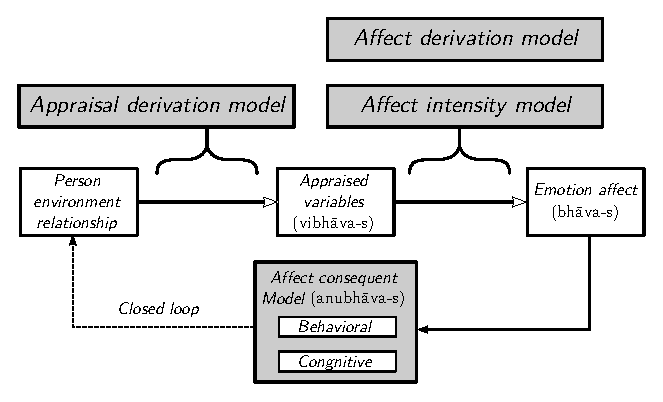
\includegraphics[scale=.85]{figures/4.eps}
\caption{A component model view of computational appraisal models (\textsl{annotated and adapted from} Marsella \textsl{et al.} (2010) \textsl{Original text in italics})}\label{chap3-fig2}
\end{figure}

We therefore start by discussing commonalities across some art forms to rebut Pollock’s\index{Pollock, Sheldon} claim that there is nothing common (\S\ref{chap3-sec1.3}). We follow with a brief summary of \textsl{Rasa} Theory\index{Rasa Theory@\textsl{Rasa} Theory} (\S\ref{chap3-sec2}) as needed for our purposes. We then give a high level outline of a theory for \textsl{rasa} (\S\ref{chap3-sec3}). We then briefly discuss current theories of mind relevant to \textsl{rasa} (\S\ref{chap3-sec3.1}). We next present an outline of our thesis towards a contemporaneous computational theory of \textsl{rasa}\index{rasa@\textsl{rasa}} (\S\ref{chap3-sec4}). Afterwards, we discuss structuring models in various Indic art forms (\S\ref{chap3-sec4.1}) followed by a computer systems model for \textsl{nāṭya}\index{natya@\textsl{nāṭya}} (\S\ref{chap3-sec4.2}), and end by giving some examples from music in \S\ref{chap3-sec4.3}. Next we discuss computational thinking specifically in the context of poetry (\S\ref{chap3-sec5.1}), music (\S\ref{chap3-sec5.2}), architecture (\S\ref{chap3-sec5.3}), and briefly in some other selected areas (\S\ref{chap3-sec5.4}). We finally end with some conclusions (\S\ref{chap3-sec6}). As to the wellsprings of Indic thinking, we then briefly discuss computational thinking as an important source: first in general (Appendix \ref{chap3-app1}), followed by computational thinking in the Indic tradition (Appendix \ref{chap3-app2}). 

As this paper is very much a work in progress, we hope that future progress in this area find a computational perspective useful.

\subsection{Commonalities across Painting and other Arts as per \textsl{Citra-sūtra}}\label{chap3-sec1.3}
\index{Citrasutra@\textsl{Citra-sūtra}}

The \textsl{Citra-sūtra}, a subtreatise of \textsl{Viṣṇudharmottara-purāṇa}\index{Visnudharmottarapurana@\textsl{Viṣṇudharmottara Purāṇa}} on painting and making images, discusses (in Chapter 43) \textsl{rasa}-s\index{rasa@\textsl{rasa}} in painting based on \textsl{Nāṭyaśāstra}.\index{Natyasastra@\textsl{Nāṭyaśāstra}} It begins with king Vajra seeking knowledge from sage Mārkaṇḍeya on the art of making images for worship so that the images manifest the deities. Mārkaṇḍeya says that without knowledge of painting, it is not possible. When he is in turn asked about painting, he says without knowing the dance art form, it is not possible as both art forms require the world to be represented. To learn dance, music, both instrumental and vocal, need to be mastered; then, mastery is also required of classical, vernacular and popular music. Thus painting is needed to understand \textsl{nāṭya};\index{natya@\textsl{nāṭya}} without knowledge of \textsl{nāṭya}, one can scarcely understand the technique of painting\endnote{It is humbling or sobering to realize that Śārṅgadeva\index{Sarngadeva@Śārṅgadeva} has \textsl{pindotpatti} as the 2nd \textsl{prakarana} of the 1st \textsl{adhyāya} in his \textsl{Saṅgītaratnākara}\index{Sangitaratnakara@\textsl{Saṅgīta-ratnākara}} as \textsl{nāda} is produced in the human body, hence the body has to be fully described first!}. 

Furthermore, he says that

\begin{myquote}
“He who does not know properly the rules of \textsl{Chitra} (painting) can scarcely discern the essentials of the images (\textsl{śilpa}).” 

\newpage

Also, 

“The observation of nature and of the rules of dancing are indicated as the ultimate resources of the painter. This does not mean that the positions of dancers have to be painted. None of the nine positions of the treatise on painting in the \textsl{Viṣṇudharmottara} coincides with any of the 101 positions explicitly described in Bharata's \textsl{Nāṭyaśāstra}. What is meant by the derivation of painting from dancing is that movement is common to both these expressive forms; it asserts itself in purity through dancing, it guides the hand of the artist, who knows how to paint figures, as if breathing, the wind as blowing, the fire as blazing, and the streamers as fluttering. The moving force, the vital breath, the life-movement (\textsl{cetana}), that is what is expected to be seen in the work of a painter, to make it alive with rhythm and expression. Imagination, observation and the expressive force of rhythm are meant by the legends of the origin of painting, to be its essential features.” \hfill (Kramrisch 1928:9--10)
\end{myquote}

A basic review of the commonality across the various \textsl{kalā}-s is also given by Sreenivasa Rao:

\begin{myquote}
“The Shilpa (sculpture) and Chitra (painting) are closely related to Nāṭya (dance)[...]. The rules of the iconography (prathima lakṣana) appear to have been derived from the Natya-sastra. The Indian sculptures are often the frozen versions or representations of the gestures and poses of dance (cāris and karaṇas) described in Natya-sastra. The Shilpa and Citra (just as the Natya)\index{natya@\textsl{nāṭya}} are based on a system of medians (sutras), measures (mānas), postures of symmetry (bhaṅgas) and asymmetry (abhaṅga, dvibhaṅga and tribhaṅga); and on the sthanas (positions of standing, sitting, and reclining). The concept of perfect symmetry is present in Shilpa and Citra as in Nrittya; and that is indicated by the term Sama.” Furthermore, “The Indian art that rendered religious themes shared a common pool of symbols and avoided imitation of the physical and ephemeral world of the senses. For instance, in all the Hindu, Jaina and Buddhist themes, alike, the Chakra -- the revolving wheel of time symbolizes the cyclical rhythms of all existence; the Padma -- or the lotus embodies creation -- that springs from the bosom of the earth; the Ananta (represented as a snake) symbolizes water -- the most important life-giving force from which all life emerges, evolves and then resolves; the Swastika – represents the four-fold aspects of creation, motion and a sense of stability; the Purnakalasha the overflowing pot symbolizes creativity and prosperity; the Kalpalata and Kalpavriksha -- the wish-fulfillment creeper symbolize imagination and creativity; and, Mriga -- or deer – symbolizes desire and beauty.

\newpage

Similarly there were a common set of gestures (mudra) by position of fingers, hands, limbs; and by stance of images in paintings and in sculptures. These varied mudras made explicit the virtues such as wisdom, strength, generosity, kindness and caring etc. The objects depicted in Indian art evoked an imagery or represented an idea that sprang from the mind. That might perhaps explain the relative absence of portraiture and even when it was attempted the emphasis was on the ideal person behind the human lineaments rather than on the physical likeness.

Another feature is the absence of the sculptures and other representations of rulers or rich patrons. And, hardly any sculpture or painting bears the signature or the name of its creator. That might again symbolize a move from particular to the universal. But, it surely baffled generations of historians.”
\end{myquote}

There is already a hint of \textsl{sādhāranīkaraṇa} of the \textsl{Rasa} Theory here; we will discuss this in detail later. Additionally, while Pollock concentrates on \textsl{praśasti} to emphasize feudal relations, here we have a different perspective. 

Furthermore, 

\begin{myquote}
“Indian figurative art is therefore not mere portraiture of the specific; but is a symbol pointing to a larger principle. It is akin to the finger pointing to the moon. For instance the image or the painting of the Buddha could be seen as that of the Buddha the historical prince Siddhartha Gotama and Sakyamuni. But, it is more than that. The Buddha figure is the embodiment of all the compassion, pathos and grace in absolute. Often, certain symbols surrounding the Buddha-image are meant to amplify its message. For instance, the idea of reverence and holiness could be represented sometimes by the surrounding vegetation, flora, fauna, yakshis, gandharvas, and apsaras each playing a specific role in building a totality; or it may be the single austere simple statement of the still centre of peace and enlightenment suggested through the symbols of the Buddha such as the Bodhi tree, seat, umbrella, sandals, footprints etc. The Buddha image is, thus, at once particular and universal. The spirit and soul of the Buddha is contained in the body of the particular but impersonalized form; the serene mood of compassion it portrays is everlasting and universal.”\hfill Rao (2012)
\end{myquote}

This again hints at \textsl{sādhāranīkaraṇa} as an important overarching principle. The sacred dimension is also an important common part across various \textsl{kalā}-s.\index{kala@\textsl{kalā}} To quote from Stella Kramrisch (1928:3):\index{Kramrisch, Stella}

\newpage

\begin{myquote}
“Vajra said: The Supreme Deity has been described as devoid of form, smell and emotion and destitute of sound and touch so how this form can be (made) of Him? Mārkaṇḍeya replied: Prakṛti and Vikṛti (come into existence) through the (variation in) the form of the Supreme Soul. That form of Him(which is) scarcely to be perceived is called Prakṛti. The whole universe should be known as the Vikrti (i.e., modification) of Him, when endowed with form. Worship and meditation (of the Supreme Being) are possible (only when He is) endowed with form. The best position of the (Supreme) Soul (however) is to be imagined without form. For seeing worlds (He) possesses eyes closed in meditation... 

This concession being made, life in its entirety becomes fit for artistic representation, and the realm of imagination is as close within the reach of the artists, as nature that surrounds him, for tradition guides him in the one case and observation checks and inspires him in the other. 
\end{myquote}

Interestingly, the cross-\textsl{kalā}\index{kala@\textsl{kalā}} aspects are also very much on the table for discussion:

\begin{myquote}
Colour symbolism underlies not only the painting of statues which, according to their \textsl{sāttvika, rājasika} and \textsl{tāmasika} aspects, had to be painted white, red or dark, but was respectively selected for \textsl{rasa}-Citras, the pictures of emotions, which, according to the Śilparatna, formed a group by themselves, distinct from the realistic paintings that were resembling what is actually seen in nature and looked like a reflex in a mirror. Each \textsl{rasa}\index{rasa@\textsl{rasa}} (emotion) had to be painted in its expressive colour, the \textsl{śṛṅgāra}\index{srngara@\textsl{śṛṅgāra}}\index{rasa@\textsl{rasa}!srngara@\textsl{śṛṅgāra}} (erotic) was of \textsl{śyāma} hue, the laugh-exciting (hāsa)\index{hasa@\textsl{hāsa}}\index{bhava@\textsl{bhāva}!hasa@\textsl{hāsa}} of white colour, the pathetic (karuṇa)\index{karuna@\textsl{karuṇa}}\index{rasa@\textsl{rasa}!karuna@\textsl{karuṇa}} of grey colour, the furious (rudra) of red colour, the heroic (vīra)\index{vira@\textsl{vīra}}\index{rasa@\textsl{rasa}!vira@\textsl{vīra}} of yellowish white colour, tho fearful (bhayānaka)\index{bhayanaka@\textsl{bhayānaka}}\index{rasa@\textsl{rasa}!bhayanaka@\textsl{bhayānaka}} of black colour, the supernatural and amazing of yellow colour and the repulsive (loathsome, vībhatsa)\index{bibhatsa@\textsl{bībhatsa}}\index{rasa@\textsl{rasa}!bibhatsa@\textsl{bībhatsa}} of blue colour.

\hfill Kramrisch\index{Kramrisch, Stella} (1928:19) (\textsl{italics and diacritics as in the original})
\end{myquote}

Kramrisch says further (1928:206b):

\begin{myquote}
The temple builder and the image maker were working on the same foundation of a magical suggestiveness of form-connections. But the rules valid for both, apply to painting too, as far as they can be applied there. ... This common basis of architecture, sculpture and painting -- it was shown that it primarily underlies dancing at times -- is responsible for a fusion of the various disciplines of sculpture and painting, for a desperate attempt of visualizing what perhaps is beyond visualisation.
\end{myquote}

\eject

The \textsl{Citra-sūtra}\index{Citrasutra@\textsl{Citra-sūtra}} concludes with an interesting observation (1928:62): 

\begin{myquote}
“In this treatise only the suggestions are given, oh king, for this subject can never be described in detail even in a hundred years. Whatever has not been said here should be inferred by other means...” 
\end{myquote}

This observation may be alluding, among many others, to the need for many \textsl{guru-śiṣya paramparā}-s to explore multiple possibilities given the basic structures; this sociological aspect is also common across various \textsl{kalā}-s\index{kala@\textsl{kalā}} due to the importance of \textsl{mano-dharma}\index{manodharma@\textsl{mano-dharma}} in the Indic tradition. 

Considering either Indic philosophy of grammar or \textsl{Rasa} Theory,\index{Rasa Theory@\textsl{Rasa} Theory} there are surprising similarities. In the Indic tradition, the intent (or inner idea, \textsl{sphoṭa})\index{sphota@\textsl{sphoṭa}} is said to be the primary cause and then comes elaboration. In the context of \textsl{vāk}, it is elaborated as \textsl{parā},\index{para@\textsl{parā}} \textsl{paśyantī}\index{pasyanti@\textsl{paśyantī}} (that which is seen by “seers”), \textsl{madhyamā}\index{madhyama@\textsl{madhyamā}} (“inner articulation”) and \textsl{vaikharī}\index{vaikhari@\textsl{vaikharī}} (“actually spoken”). In \textsl{Rasa}/linguistic\index{rasa@\textsl{rasa}} theory, we have \textsl{sphoṭa} that corresponds to the first two, \textsl{dhvani}\index{dhvani@\textsl{dhvani}} that corresponds to the last two. What is interesting is that the commonality arises from the same source or perspective such as, for example, Kāśmīra Śaiva thinking on the nature of reality. Furthermore, Mukund Lath\index{Lath, Mukund} (2016:103) in the context of thought and music says 

\begin{myquote}
“...The idea of \textsl{paśyantī vāk} (and the word “\textsl{vāk}” here, can be plainly taken to indicate both music and word-based language: both being sound-based) suggests a level of meaning-consciousness that lies beyond the ordinary levels of language usage, beyond, in other words, of \textsl{vaikharī} (uttered, expressed language) and \textsl{madhyamā} (the unuttered flow of language that keeps endlessly moving in our consciousness). We are in the field of \textsl{paśyantī} when we are seeking to articulate an unexpressed thought---or a \textsl{rāga}.\index{raga@\textsl{rāga}} We look for the right word or \textsl{svara},\index{svara@\textsl{svara}} which is not there but which we reach through our meaning-seeking reflexive consciousness. But what is the criterion of discrimination? The criterion is the unexpressed, disembodied idea itself, for there can be no other. And this search therefore leads us beyond \textsl{paśyantī} into \textsl{parā}: for the sought idea---or \textsl{rāga}\index{raga@\textsl{rāga}}---is not a singularly existing “metaphysical” entity, it lies in an ineffable field of an ever creative possibility. This is the \textsl{parā}, the source, the seed or the nucleus of meaningfulness. We have no grasp of it, except, in whatever measure, through our inward-turning reflexive consciousness, which forever and insistently tries to reach out to it.”
\end{myquote}

The above discussion hopefully convinces the reader that lack of commonality is not a defensible proposition and it is incomprehensible that Pollock\index{Pollock, Sheldon} even makes the charge. We discuss this aspect in a more technical way below by looking at the “atomic” units of the various art forms and how they are grouped bottom up for discussing higher level structures and also the opposite top down view where appropriate.

\section{A Brief Introduction to \textsl{Rasa}}\label{chap3-sec2}

\textsl{Rasa}\index{rasa@\textsl{rasa}} can be defined as ecstasy derived from seeing or hearing an art form such as \textsl{driśya-kāvya}\index{kavya@\textsl{kāvya}}\index{drsyakavya@\textsl{dṛśyakāvya}}\index{sravyakavya@\textsl{śravyakāvya}} (e.g., \textsl{nāṭya})\index{natya@\textsl{nāṭya}} or \textsl{śravya-kāvya} (e.g., \textsl{Rāmāyaṇa}).\index{Ramayana@\textsl{Rāmāyaṇa}} \textsl{Bharatārṇava}\index{Bharatarnava@\textsl{Bharatārṇava}} of Nandikeśvara\index{Nandikesvara@Nandikeśvara} in particular says (Gairola 2013:225)

\begin{quote}
\textsl{aṅgenālambayed gītaṁ hastenārtha-pradarśanam |}\\
\textsl{cakṣurbhyāṁ bhāvayed bhāvaṁ pādābhyāṁ tāla-nirṇayaḥ ||}
\end{quote}

``The song is supported by the body;\\
The hands show the meaning;\\
The eyes express the moods;\\
The \textsl{tāla}\index{tala@\textsl{tāla}} by the feet.''
\begin{quote}
\textsl{yato hastas tato dṛṣṭir yato dṛṣṭis tato manaḥ |}\\
\textsl{yato manas tato bhāvo yato bhāvas tato rasaḥ ||}
\end{quote}

``Where the hand is, the eyes follow; where the eyes go, the mind follows; where the mind is, there the \textsl{bhāva}\index{bhava@\textsl{bhāva}} is; where there is \textsl{bhāva}, there the \textsl{rasa}\index{rasa@\textsl{rasa}} is”.

The \textsl{anukartṛ} (actor) uses his body (e.g., \textsl{grīvā}, \textsl{bhrū}) and \textsl{cāri}, \textsl{karaṇa} (body postures) to emote the \textsl{bhāva}-s.\index{bhava@\textsl{bhāva}} The above \textsl{śloka}-s give a vivid connection between the mind and body coordination so central in a general theory of \textsl{rasa}. A reader or spectator may identify himself/herself with the characters depicted so completely that he/she may weep real tears but it is that of exquisite joy! To explain such a phenomenon, a theory of \textsl{rasa}\index{rasa@\textsl{rasa}} is needed; this is addressed at length in the Indian tradition. 

In Chapter 6 of \textsl{Nāṭyaśāstra}\index{Natyasastra@\textsl{Nāṭyaśāstra}} (6.33-6.34), Bharata\index{Bharatamuni}
 says that \hbox{\textsl{bhāva}-s}\index{bhava@\textsl{bhāva}} produce \textsl{rasa} and not vice versa (Rastogi 2016)! However, just immediately afterwards (6.35-37), while Bharata first says \hbox{\textsl{bhāva}-s} cause the many \textsl{rasa}-s through \textsl{abhinaya},\index{abhinaya@\textsl{abhinaya}} he then says neither is \textsl{rasa} without \textsl{bhāva}-s nor vice versa. Furthermore, in their mutual dependence, both their fullnesses result from \textsl{abhinaya}; their relationship is like that between a seed and its plant and each causes the other to happen! \textsl{Bhāva}-s and \textsl{rasa}-s cause one another to come into existence (\textsl{bhāvayanti}). These statements can be reconciled if we keep in mind the idea that while at the beginning \textsl{bhāva}-s\index{bhava@\textsl{bhāva}} cause \textsl{rasa}-s to be produced, subsequently, they can have a codependency.

Additionally, a \textsl{rasa}\index{rasa@\textsl{rasa}} is not a single “essence,” as it is not a single, pure substance but a combination of many sensory inputs; these produce “a richly textured, emotionally resonant experience larger than the sum of its parts” (Beitmen 2014). Furthermore, \textsl{rasa} is an additive property. Bharata\index{Bharatamuni} describes \textsl{rasa} using the metaphor of a mixture: \textsl{rasa} is like the agreeable taste of a well made dish with spices, with the aesthetic experience being the savoring of this dish. Different \textsl{bhāva}-s (emotional states) such as \textsl{hāsya}\index{hasya@\textsl{hāsya}}\index{rasa@\textsl{rasa}!hasya@\textsl{hāsya}} and \textsl{śṛṅgāra}\index{srngara@\textsl{śṛṅgāra}}\index{rasa@\textsl{rasa}!srngara@\textsl{śṛṅgāra}} are like ingredients in the dish; although they are mixed, \textsl{sahṛdaya}-s\index{sahrdaya@\textsl{sahṛdaya}} can distinguish each emotion while at the same time enjoying their creative combination. Bharata’s \textsl{rasa} model is therefore the aesthetics of a mixture of emotions and not pure essences (Beitman 2014:30--31). Moreover, Bharata declares that the various \textsl{rasa}-s (the “moods” experienced by the audience members) and the \textsl{bhāva}-s (the “states of being” portrayed by the actors) “cause one another to originate (\textsl{bhāvayanti})”. 

Bharata\index{Bharatamuni} has listed 56 \textsl{bhāva}-s\index{bhava@\textsl{bhāva}} and 8 \textsl{rasa}-s.\index{rasa@\textsl{rasa}} For example, \textsl{rati} \textsl{bhāva}\index{bhava@\textsl{bhāva}!rati@\textsl{rati}}\index{rati@\textsl{rati}} and its corresponding \textsl{śṛṅgāra}\index{srngara@\textsl{śṛṅgāra}}\index{rasa@\textsl{rasa}!srngara@\textsl{śṛṅgāra}} \textsl{rasa}; similarly \textsl{utsāha bhāva/vīra\index{bhava@\textsl{bhāva}!utsaha@\textsl{utsāha}}\index{utsaha@\textsl{utsāha}} rasa;\index{vira@\textsl{vīra}}\index{rasa@\textsl{rasa}!vira@\textsl{vīra}} śoka/karuṇa;\index{karuna@\textsl{karuṇa}}\index{rasa@\textsl{rasa}!karuna@\textsl{karuṇa}} hāsa/hāsya;\index{hasya@\textsl{hāsya}}\index{rasa@\textsl{rasa}!hasya@\textsl{hāsya}}\index{hasa@\textsl{hāsa}}\index{bhava@\textsl{bhāva}!hasa@\textsl{hāsa}} vismaya/adbutha}.\index{adbhuta@\textsl{adbhuta}}\index{rasa@\textsl{rasa}!adbhuta@\textsl{adbhuta}}\index{vismaya@\textsl{vismaya}}\index{bhava@\textsl{bhāva}!vismaya@\textsl{vismaya}} These are \textsl{kāyika} or \textsl{āngika bhāvas}. Examples of \textsl{anaṅgi rasa}-s are \textsl{bhaya/bhayānaka,\index{bhayanaka@\textsl{bhayānaka}}\index{rasa@\textsl{rasa}!bhayanaka@\textsl{bhayānaka}}\index{bhava@\textsl{bhāva}!bhaya@\textsl{bhaya}}\index{bhaya@\textsl{bhaya}} krodha/raudra,\index{raudra@\textsl{raudra}}\index{rasa@\textsl{rasa}!raudra@\textsl{raudra}}\index{bhava@\textsl{bhāva}!krodha@\textsl{krodha}}\index{krodha@\textsl{krodha}} jugupsā/bībhatsa};\index{bibhatsa@\textsl{bībhatsa}}\index{rasa@\textsl{rasa}!bibhatsa@\textsl{bībhatsa}}\index{bhava@\textsl{bhāva}!jugupsa@\textsl{jugupsā}}\index{jugupsa@\textsl{jugupsā}} interestingly, some of these are said to be implicated in psychological disorders. Some \textsl{bhāvas} are \textsl{sāttvika}\index{sattvikabhava@\textsl{sāttvikabhāva}} such as \textsl{romancaka, stambha, vaivarṇya};\index{sattvikabhava@\textsl{sāttvikabhāva}!romancaka@\textsl{romancaka}}\index{sattvikabhava@\textsl{sāttvikabhāva}!vaivarnya@\textsl{vaivarṇya}}\index{sattvikabhava@\textsl{sāttvikabhāva}!stambha@\textsl{stambha}} these depict the physical expression of the emotions in the mind.

There are primary or stable \textsl{bhāva-s (sthāyibhāva-s)}\index{sthayibhava@\textsl{sthāyibhāva}} and secondary or transitory ones (\textsl{sañcāribhāva-s}).\index{sancaribhava@\textsl{sañcāribhāva}} \textsl{sthāyibhāva-s} are stable emotions that can become \textsl{rasa}-s;\index{rasa@\textsl{rasa}} \textsl{Śrī Bhakti-rasāmṛta-sindhu}\index{Sri Bhaktirasamrtasindhu@\textsl{Śrī Bhakti-rasāmṛta-sindhu}} (2.5.1) gives the following definition:
\begin{quote}
\textsl{aviruddhān viruddhāṁś ca bhāvān yo vaśatāṁ nayan} |\\
\textsl{su-rājeva virājeta sa sthāyi bhāva ucyate} ||
\end{quote}

\newpage

“That \textsl{bhāva} which, controlling other favorable \textsl{bhāva}-s\index{bhava@\textsl{bhāva}} such as \textsl{hāsya},\index{hasya@\textsl{hāsya}}\index{rasa@\textsl{rasa}!hasya@\textsl{hāsya}} and contradictory \textsl{bhāva}-s such as \textsl{krodha},\index{bhava@\textsl{bhāva}!krodha@\textsl{krodha}}\index{krodha@\textsl{krodha}} presides in the manner of an efficient ruler, is called the \textsl{sthāyibhāva}.”\index{sthayibhava@\textsl{sthāyibhāva}} The \textsl{sthāyibhāva}-s are caused to happen by the actor (\textsl{bhāvayanti iti bhāvāḥ}) so that the related \textsl{rasa}\index{rasa@\textsl{rasa}} is produced in the spectator (\textsl{bhavanti iti bhāvāḥ}); these require, in a good performance, that there is correspondence between the cognitive\endnote{In Indic thought, we have \textsl{manas} (“supervisor” of the 5 \textsl{karmendriya}-s\index{karmendriya@\textsl{karmendriya}} and 5 \hbox{\textsl{jñānendriya}-s)},\index{jnanendriya@\textsl{jñānendriya}} \textsl{citta}\index{citta@\textsl{citta}} (store of sense impressions), \textsl{ahaṅkāra}\index{ahankara@\textsl{ahaṅkāra}} (I-am-ness), \textsl{buddhi}\index{buddhi@\textsl{buddhi}} (decision maker that may control \textsl{manas}, \textsl{citta} and \textsl{ahaṅkāra}). “Cognitive” here may be taken to be all of these aspects as they deal with the representational aspects. In a computer systems perspective, these are roughly the input-output (I/O) controller, persistent storage, thread of control, and the code/algorithms of the core kernel. Only the network aspect is not explicitly mentioned as it is possibly subsumed by the I/O controller.}/mental states of both the actor and spectator. It is interesting that \textsl{Nāṭyaśāstra}\index{Natyasastra@\textsl{Nāṭyaśāstra}} also discusses certain physical states of the spectator in the context of \textsl{rasa} including sounds (claps, counting \textsl{tāla},\index{tala@\textsl{tāla}} \textsl{aho}!, etc) and movements (hands, head, etc); this is another instance where the Indic world differs in that total silence is not expected from the audience!

\textsl{Viṣṇu-dharmottara}\index{Visnudharmottarapurana@\textsl{Viṣṇudharmottara Purāṇa}} says it in its own way:
\begin{quote}
\textsl{rasānāṁ samavetānāṁ yasya rūpaṁ bhaved bahu} |\\
\textsl{sa mantavyo rasaḥ sthāyī śeṣaḥ sañcāriṇo mataḥ} ||
\end{quote}

When \textsl{rasa}-s\index{rasa@\textsl{rasa}} come together, the \textsl{rasa} whose nature is prominent is the \textsl{sthāyibhāva}, and the other \textsl{rasa}-s are \textsl{sañcāribhāva}-s.\index{sancaribhava@\textsl{sañcāribhāva}}

\textsl{Rasa} is not \textsl{ādhyātmika} but at the same time it is not \textsl{laukika}.\index{laukika@\textsl{laukika}} Abhinavagupta\index{Abhinavagupta} extended the original 8 \textsl{rasa}s of Bharata\index{Bharatamuni} by adding \textsl{śānta\index{rasa@\textsl{rasa}!santa@\textsl{śānta}}\index{santarasa@\textsl{śāntarasa}} rasa. Rasānanda} or \textsl{kāvyānanda/kalānanda} is held to be different from \textsl{brahmānanda} but more like \textsl{śānta rasa}; here \textsl{ānanda} is defined as that \textsl{sukha} that is not \textsl{duḥkha-sparśi-sukha} (that which is untouched by sorrow). Later, \textsl{śānta rasa} (Abhinavagupta) and \textsl{bhakti\index{rasa@\textsl{rasa}!bhakti@\textsl{bhakti}}\index{bhaktirasa@\textsl{bhakti-rasa}} rasa} (Rūpa\index{Rupa Gosvamin@Rūpa Gosvāmin} Gosvāmin/Madhusūdana\index{Madhusudana Sarasvati@Madhusūdana Sarasvatī} Sarasvati) have been held to be close to the state of \textsl{mokṣa}. But Bharata’s \textsl{rasa} is in the domain of \textsl{dharma} (\textsl{trivarga}) and not \textsl{mokṣa}\endnote{The Veda-s\index{Veda-s@\textsl{Veda}-s} also discuss \textsl{soma-rasa};\index{somarasa@\textsl{soma-rasa}} only the \textsl{soma-rasa} is close to \textsl{śānta/bhakti rasa}\index{santa@\textsl{śānta}}\index{rasa@\textsl{rasa}!santa@\textsl{śānta}}\index{bhakti@\textsl{bhakti}}\index{rasa@\textsl{rasa}!bhakti@\textsl{bhakti}} and not to others. However, this has been mistranslated as spirituous by European Indologists; this is unfortunate as it is very different from \textsl{mada} (such as \textsl{ariṣṭa or āsava}) (Nagaraj\index{Nagaraj, P.} 2016).}!\endnote{We briefly list the usage of the word \textsl{rasa}\index{rasa@\textsl{rasa}} in the \textsl{Trayī} which is different from what we have discussed so far. \textsl{Taittirīya Upaniṣad}\index{Taittiriyopaniṣad@\textsl{Taittirīyopaniṣad}}\index{Upanisad@\textsl{Upaniṣad}!Taittiriya@\textsl{Taittirīya}} (2.7.1) says 
\begin{quote}
\textsl{yad vai tat sukṛtaṁ} |\\ 
\textsl{raso vai saḥ} |\\
\textsl{rasaṁ hy evāyaṁ labdhvā’’nandī bhavati} ||
\end{quote}
\begin{myquote}
“That which is known as the self-creator is verily the source of joy [\textsl{rasa}]; for one becomes happy by coming in contact with that source of joy [\textsl{rasa}]” (Gambhirananda\index{Gambhirananda, Swami} 2000:360).
\end{myquote}

Alternately, \textsl{raso vai saḥ} here has also been translated as “Truly, the Lord is \textsl{rasa}".

Kṛṣṇa\index{Krsna@Kṛṣṇa} in the \textsl{Gītā} (7.8)\index{Bhagavadgita@\textsl{Bhagavad-gītā}} says he is the \textsl{rasa} in water, pointing out the subtlety of \textsl{rasa}: not easy to describe as it can only be experienced:
\begin{quote}
\textsl{raso’ham apsu kaunteya, prabhāsmi śaśi-sūryayoḥ} |\\
\textsl{praṇavaḥ sarva-vedeṣu, śabdaḥ khe, pauruṣaṁ nṛṣu} ||
\end{quote}

In the earlier thinking on \textsl{rasa}, like \textsl{asat} (\textsl{asad vā idam agra āsīt} | \textsl{tato vai sad ajāyata} \textsl{Taittirīya Upaniṣad}\index{Taittiriyopaniṣad@\textsl{Taittirīyopaniṣad}} 
\index{Upanisad@\textsl{Upaniṣad}!Taittiriya@\textsl{Taittirīya}} 2.7.1) or \textsl{dharma}, \textsl{rasa} is the seed, or alternatively the \textsl{yoni}, of everything, given its identification with the self-creator or the Lord.}

Bharata says: “\textsl{vibhāvānubhāva-vyabhicāri-saṁyogad rasa-niṣpattiḥ}”\break which is typically translated as follows\endnote{Note some similarity with Appraisal Theory in the technical area of affective computing (Marsella 2010): “In appraisal theory, emotion is argued to arise from patterns of individual judgement concerning the relationship between events and an individual’s beliefs, desires, and intentions, sometimes referred to as the \textsl{person–environment relationship } (Lazarus 1991) [\textsl{vibhāva}-s].\index{vibhava@\textsl{vibhāva}} These judgements, formalized through reference to devices such as \textsl{situational meaning structures} or \textsl{appraisal variables} (Frijda 1987), characterize aspects of the personal significance of events. Patterns of appraisal are associated with specific physiological and behavioural reactions [\textsl{anubhāva}-s].\index{anubhava@\textsl{anubhāva}} In several versions of appraisal theory, appraisals also trigger cognitive responses [\hbox{\textsl{sañcāribhāva}-s?}],\index{sancaribhava@\textsl{sañcāribhāva}} often referred to as \textsl{coping strategies}--e.g. planning, procrastination, or resignation—feeding back into a continual cycle of appraisal and reappraisal (Lazarus 1991:127).” But the notion of \textsl{rasa} is either not present or not clearly articulated.}: \textsl{rasa}\index{rasa@\textsl{rasa}} is said to be produced (\textsl{rasa-niṣpattiḥ}) by a combination of the \textsl{vibhāva}\index{vibhava@\textsl{vibhāva}} (determinants), \textsl{anubhāva}\index{anubhava@\textsl{anubhāva}} (consequents), and \textsl{vyabhicāribhāva}\index{vyabhicaribhava@\textsl{vyabhicāribhāva}} (\textsl{sañcāri}\index{sancaribhava@\textsl{sañcāribhāva}} or transitory states or fleeting emotions). Some \textsl{vibhāva-}s are \textsl{ālambana} (supporting), some are \textsl{uddīpana} (intensifying; usually environmental ones).

\textsl{Avadhāni} Shankar Rajaraman says:

\begin{myquote}
From an Indian aesthetic viewpoint, narratives can be understood in terms of the emplotment of \textsl{vibhāva}-s (antecedent events), \textsl{anubhāva}-s (consequent responses including verbal and non-verbal behaviours), and \textsl{vyabhicāri-bhava}-s (transient states such as \textsl{garva}, \textsl{asūyā}, \textsl{śrama}, \textsl{vyādhi}, \textsl{viṣāda}). Put simply, Sanskrit poets integrate \textsl{vibhāva}-s,\index{vibhava@\textsl{vibhāva}} \textsl{anubhāva}-s,\index{anubhava@\textsl{anubhāva}} and \textsl{vyabhicāri}-\textsl{bhava}-s\index{vyabhicaribhava@\textsl{vyabhicāribhāva}} in a coherent and meaningful manner within a narrative. The effect of emplotment on the reader is that his/her \textsl{sthāyi}-\textsl{bhāva}-s (sustained egocentric mental states such as \textsl{rati},\index{rati@\textsl{rati}}\index{utsaha@\textsl{utsāha}}\index{soka@\textsl{śoka}} \textsl{utsāha} (perseverence), \textsl{śoka} (sorrow)) are transformed into \textsl{rasa}-s -- their pleasurable, aesthetic counterparts. According to the \textsl{Nāṭya-śāstra}\index{Natyasastra@\textsl{Nāṭyaśāstra}} of Bharatamuni\index{Bharatamuni} (1992), dramatic narrative (\textsl{nāṭya}) must refer to the actual world for its depiction of antecedent events and consequent responses. \textsl{Vibhāva}-s and \textsl{anubhāva}-s thus have their real world correspondences in the form of \textsl{kāraṇa}-s and \textsl{kārya}-s. To know \textsl{vibhāva}-s and \textsl{anubhāva}-s is to know their corresponding real world \textsl{kāraṇa}-s and \textsl{kārya}-s (stimuli and responses). \textsl{Vibhāva}-s and \textsl{anubhāva}-s are therefore described by Bharatamuni (Dvivedi 1996:153) as \textsl{loka-svabhāvānugata} (compatible with what holds true in the actual world), \textsl{loka-prasiddha} (well-established in the actual world), \textsl{loka-svabhāva- saṁsiddha} (determined by what holds true in the actual world), and \textsl{loka-yātrānugāmi} (in agreement with the world of interactions). The word \textsl{loka} (world) used here refers, no doubt, to a cultural world within which \textsl{nāṭya}\index{natya@\textsl{nāṭya}} is made meaningful. 

\hfill(Shankar 2018:224)
\end{myquote}

After Bharata,\index{Bharatamuni} many thinkers such as Daṇḍin,\index{Dandin@Daṇḍin} Bhaṭṭa Nāyaka,\index{Bhatta Nayaka@Bhaṭṭa Nāyaka} Ānandavardhana,\index{Anandavardhana@Ānandavardhana} Abhinavagupta\index{Abhinavagupta} and others discussed the use and application of the theory of \textsl{rasa}\index{rasa@\textsl{rasa}} to literary texts but with their own innovations. For example, Ānandavardhana introduced a new thinking into \textsl{kāvya}\index{kavya@\textsl{kāvya}}
 that a poet ought to strive to evoke a single \textsl{rasa}; this predominant \textsl{rasa} he called \textsl{aṅgi-rasa}.\index{angirasa@\textsl{aṅgi-rasa}}\index{rasa@\textsl{rasa}!angirasa@\textsl{aṅgi-rasa}} Even if other \textsl{rasa}-s are necessary, those should be treated as mere auxiliary to the main \textsl{rasa}. Furthermore, a plot also must have a \textsl{aṅgi-rasa} with good \textsl{kāvya} avoiding those aspects not directly relevant to the development of the main theme and \textsl{rasa} (such as events, descriptions, figures of speech, etc.). Bharata\index{Bharatamuni} did not have this requirement: there could be different \textsl{rasa}-s as needed in a dramatic production. Other authors developed this idea further; even here, it seems that each act in a dramatic performance would have a principal \textsl{rasa}. 

As an example, we now give one \textsl{rasa}\index{rasa@\textsl{rasa}} based analysis in a \textsl{kāvya}, again from Shankar (Shankar 2018:228):

\begin{myquote}
...[V]erse no. 1.1, the \textsl{nāndī-padya}, of Harṣa’s\index{Sriharsa@Śrīharṣa} \textsl{Priyadarśikā}...\index{Priyadarsika@\textsl{Priyadarśikā}} depicts the marriage between Śiva and Pārvatī, describing a series of emotional states that the latter is going through in that situation. Pārvatī, the bride, longs to have a look at the face of Śiva, the groom. But her eyes are agitated by the smoke from the sacrificial fire. The cool rays of the moon on Śiva’s head come to her rescue and comfort her reddened eyes. Just as she is about to catch a glimpse of Śiva’s face, she beholds Brahmā, the officiating priest, in their vicinity, and out of modesty bends her face down (how could she, in spite of her eagerness, directly look at the groom when another male is standing close by?). She can now see Śiva reflected in her bright toe-nails. But instead of being happy that she could manage to look at least at the reflected image of her husband, Pārvatī is filled with jealousy because along with Śiva is also reflected Gaṅgā, her co-wife, whom he holds in his matted locks. Going through these emotional states, Pārvatī suddenly feels the touch of Śiva’s hand on hers during the ritual of \textsl{pāṇi-grahaṇa} and is covered by goosebumps. [The] poet has carefully brought together the descriptions of several bodily and behavioral responses (agitated eyes, bending the face down, goosebumps) and mental states (eagerness, bashfulness, jealousy) to strengthen his depiction of Pārvatī’s love for Śiva (In \textsl{Nāṭyaśāstric} terms, the \textsl{sthāyi-bhāva}\index{sthayibhava@\textsl{sthāyibhāva}} in this verse is \textsl{rati},\index{rati@\textsl{rati}} which being augmented by \textsl{vyabhicāri-bhāva}-s\index{vyabhicaribhava@\textsl{vyabhicāribhāva}} such as \textsl{autsukya},\index{autsukya@\textsl{autsukya}} \textsl{vrīḍā}\index{vrida@\textsl{vrīḍā}} and \textsl{asūyā},\index{asuya@\textsl{asūyā}} and \textsl{anubhāva}-s such as agitated eyes, bending the face down, goosebumps, etc., is elevated to the state of the \textsl{rasa} viz.\ \textsl{śṛṅgāra} in the reader.)
\end{myquote}

Another example we can give is that of Lalleśvarī (Lal Ded)\index{Lalleshvari (Lal Ded)@Lalleśvarī (Lal Ded)} of Kāśmīr. In one of her \textsl{vāk-}s, she says (Hoskote 2011:134):

\begin{myquote}
So many times I’ve drunk the wine of the Sindhu river.

So many roles I’ve played on this stage.

So many pieces of human flesh I’ve eaten.

But I’m still the same Lalla, nothing’s changed.
\end{myquote}

On a first reading, \textsl{bhayānaka}\index{bhayanaka@\textsl{bhayānaka}}\index{rasa@\textsl{rasa}!bhayanaka@\textsl{bhayānaka}} (terrifying) or \textsl{bībhatsa}\index{bibhatsa@\textsl{bībhatsa}}\index{rasa@\textsl{rasa}!bibhatsa@\textsl{bībhatsa}} (disgusting) \hbox{\textsl{rasa}-s}\index{rasa@\textsl{rasa}} are likely. A deeper explanation is interesting: Lalla’s\index{Lalleshvari (Lal Ded)@Lalleśvarī (Lal Ded)} \textsl{ātman} has used/consumed so many bodies in her past lives!

One cannot fail to notice that \textsl{rasa} is often discussed taxonomically in the Indic tradition (for example, 56 \textsl{bhāva}-s\index{bhava@\textsl{bhāva}} or 9 \textsl{rasa}-s); interestingly many of these distinctions are surprisingly well founded (the list of \textsl{bhāva}-s/\textsl{rasa}-s says Patrick Hogan\index{Hogan, Patrick} “coincides remarkably well with the lists of “basic emotions” developed by cognitive psychologists in recent years (see, for example, Ekman\index{Ekman, Paul}\endnote{In 1972, Ekman\index{Ekman, Paul} had listed (1972:251) the following emotions: Anger, Disgust, Fear, Happiness, Sadness, and Surprise. However, in the 1990s Ekman expanded his list of basic emotions, including a range of positive and negative emotions not all of which are encoded in facial muscles. The newly included emotions are: Amusement Contempt, Contentment, Embarrassment, Excitement, Guilt, Pride in achievement, Relief, Satisfaction, Sensory pleasure, Shame. Ekman has been also working since the last 2 decades in the area of “microexpressions”. (Ekman 1999:55).}; Oatley and Johnson-Laird; and Johnson-Laird and Oatley)” (Hogan 2003a:40). The Indic taxonomical impulse is due to its inclusive orientation so as not to exclude anything; Hogan makes an interesting observation on Indian ontology and epistemology that is worth quoting here:

\begin{myquote}
“While all cultures are diverse, India has reveled in its differences. Ancient sages sparred with one another on every question from the meaning of the universe and the nature of soul to the precise number of the varieties of the simile. One may draw a broad distinction between exclusionary cultures and incorporative cultures. Exclusionary cultures tend to identify a “correct” set of practices and to eliminate others. Incorporative cultures tend to accept all varieties of idea and habit, finding a singular place for them — often in a hierarchical structure. Ancient, classical and medieval India are among the most incorporative cultures of which I am aware. Thus, historically, India has been culturally multiple not only in lived culture, but in official culture. Indeed, some of the greatest intellectual achievements of ancient India come from an attempt to systematize that diversity. The theories of \textsl{rasa} and \textsl{dharma} are two primary instances of that systematization.”  
\hfill(Hogan\index{Hogan, Patrick} 2003a:39)
\end{myquote}

\vskip .2cm

\section{A High Level Theory for \textsl{Rasa}}\label{chap3-sec3}
\index{rasa@\textsl{rasa}}

\vskip .1cm

In this paper, we argue for a computational cum cognitive basis for \textsl{rasa} as an important component underlying \textsl{rasa}’s theoretical foundations in the Indic tradition and that such a model, we believe, addresses well the issues raised by Pollock\index{Pollock, Sheldon} above to understand the wellsprings of \textsl{pratibhā} as well as the commonality across \textsl{kalā}-s.\index{kala@\textsl{kalā}} For \textsl{rasa}, there is a generation aspect as well as a recognition aspect. For the generative part, the computational cum cognitive aspect is at two levels: at a cognitive level when the art form is performed and at a design level when the art form is created. Also it should be noted that our argument is not only that the \textsl{rasa} felt by a spectator (“at run-time”) has to be partly cognitively structured and therefore supporting cognitive models may be necessary, but also that the creator (“at design-time”) needs to understand how to create structures that create the right \textsl{rasa}\index{rasa@\textsl{rasa}} in the spectator, or the right \textsl{bhāva}\index{bhava@\textsl{bhāva}} that needs to be emoted by the actor or artist; and here is where the computational aspect comes in. This is a crucial point that needs to be kept in mind while reading this paper as we are arguing for a non-standard, possibly unfamiliar, perspective. 

\vskip .1cm

For the recognition part, either the simpler iterative structures are sensed and fused with earlier (emoted) sensations \hbox{(“\textsl{anubhāva}-s”)}\index{anubhava@\textsl{anubhāva}} by the layman or the more complex probabilistic structures are recognized “emotionally” by the \textsl{sahṛdaya}-s\index{sahrdaya@\textsl{sahṛdaya}} again given earlier \textsl{anubhāva}-s. This aspect is more closely connected with the affective component of \textsl{rasa},\index{rasa@\textsl{rasa}} the embodied sense.

\vskip .1cm

Positing a recursive nature of reality (see Vatsyayan\index{Vatsyayan, Kapila} (1997), Chapter 4, for a discussion with respect to \textsl{Nāṭyaśāstra}),\index{Natyasastra@\textsl{Nāṭyaśāstra}} a computational/cognitive style of thinking seems to have been the basis of much activity in diverse Indic disciplines. The theory of \textsl{rasa}, in terms of affecting a \textsl{bhāva}\index{bhava@\textsl{bhāva}} in the artists/creators or \textsl{rasa}\index{rasa@\textsl{rasa}} in the spectators, or constructing the art form in the first place, in turn has had a computational perspective. 

\vskip .1cm

This is with respect to the wellsprings of \textsl{pratibhā}\index{pratibha@\textsl{pratibhā}} as well as to understand the commonality across many \textsl{kalā}-s\index{kala@\textsl{kalā}} (domains); hence if our argument is sound or well attested by examples in the Indic tradition, Pollock’s\index{Pollock, Sheldon} imputations above can then be said to be colored by his somewhat consistent negative thinking with respect to Indic models notwithstanding his erudition or overt appreciation in some instances. 

\vskip .1cm

Our main argument for the cognitive component is as follows. As the Indic tradition fundamentally makes a distinction between an actual emotion of being, say, in love or in pain or feel separation (“\textsl{bhāva}”), and what is experienced through \textsl{nāṭya}\index{natya@\textsl{nāṭya}} or music or art, one can say (at the start) that the latter (“\textsl{rasa}”)\index{rasa@\textsl{rasa}} is a simulation of the earlier one (“\textsl{bhāva}”). As we continue with the performance, each such simulation (using “memory traces” of earlier \textsl{bhāva}-s) has to be stitched together in a larger structure that represents/recalls cognitive states (along with affective states). The notion of “\textsl{dhvani}”\index{dhvani@\textsl{dhvani}} builds these ideas further. \textsl{Dhvani} is a non-signifiable (or non-translatable?) "suggestion" of a word, phrase, sentence, (more generally) topic, or a situation constructed linguistically or in some specific art form (but which is quite different from the various \textsl{alaṅkāra}-s\index{alankara@\textsl{alaṅkāra}} considered in poetics). However, one cannot list all the \textsl{dhvani}-s or “suggestions”, even all the pertinent ones, of a given text or performance. Abhinavagupta\index{Abhinavagupta} also says that some memory traces may not be in the foreground consciousness but which may still have an affective component. What is even more interesting is the relevant ideas such as \textsl{sādhāraṇīkaraṇa}\index{sadharanikarana@\textsl{sādhāraṇīkaraṇa}} (“generalization”) that have a computational flavour as we have discussed.

\vskip .1cm

Our main argument for the computational aspect is as follows. The Indic mind, starting from the Vedic and Upaniṣadic times, conceived of the universe in terms of a recursive structure so that the “very small” and the “very large” could be attempted to be grasped at the same time (see Kak\index{Kak, Subhash} (2005), Malhotra\index{Malhotra, Rajiv} (2014))\endnote{For example, in the Sāṅkhya system, the \textsl{pinda}-\textsl{brahmānda} concepts map the “microcosm” to the “macrocosm”, and vice versa. In \textsl{Atharvaveda}\index{Atharvaveda@\textsl{Atharvaveda}}
\index{Veda-s@\textsl{Veda}-s!Atharvaveda@\textsl{Atharvaveda}} and in Avataṁsaka Sūtra, the recursive nature of reality, for example, is thought of as an infinite net with a crystal at each crossing that simultaneously shines light and (recursively) reflects the lights from other lights.}. Mathematically (and computationally), iteration and (more generally) recursion (or its equivalents) are necessary to capture the (Turing-complete) potential of a system built on a finite set of rules. This same Indic intuition has been helpful in developing powerful models across many disciplines that deal with \textsl{rasa}.\index{rasa@\textsl{rasa}} Furthermore, this recursive nature has some surprising or epiphenomenal properties, seemingly not present in the finite set of rules or that are not directly obvious and hence creates a sense of \textsl{rasa} that is exhilarating and worth striving for. (For a brief introduction to computational thinking and its specific Indic aspect, refer to Appendixes \ref{chap3-app1} and \ref{chap3-app2}). We give some examples of such thinking in some art forms in Section \ref{chap3-sec5}.

Starting from Bhaṭṭa Nāyaka,\index{Bhatta Nayaka@Bhaṭṭa Nāyaka} Abhinavagupta\index{Abhinavagupta} and others, it is argued that \textsl{rasa} or the aesthetic pleasure results from "generalization": the removal of non-essential aspects or the self-interest “which is part of the link between the affect and the representational content in memory traces”. Using what could be called a computational model (viz. computable functions or state machines with inputs and outputs), \textsl{rasa}\index{rasa@\textsl{rasa}} is said to be “produced” (\textsl{rasa-niṣpattih}) by a combination of the \textsl{vibhāva}\index{vibhava@\textsl{vibhāva}} (determinants), \textsl{anubhāva}\index{anubhava@\textsl{anubhāva}} (consequents), and \textsl{vyabhicāri-bhāva}\index{vyabhicaribhava@\textsl{vyabhicāribhāva}} (transitory states or fleeting emotions). 

By a process of abstraction (called \textsl{sādhāraṇīkaraṇa}\index{sadharanikarana@\textsl{sādhāraṇīkaraṇa}} “generalization”), particulars are dropped; this is useful as it is said that common everyday constraints (e.g., time, place, person’s emotional moods, etc) limit the experience of \textsl{rasa}. This abstraction allows us to go to the core of the experience itself (a related example in Vedānta is the removal of the “\textsl{avidyā}” clouding our thinking). An analogous method in programming languages is “program slicing” where a program is “simplified” in a consistent way to remove a variable. 

Furthermore, prototypes have been proposed by later commentators on \textsl{rasa}\index{rasa@\textsl{rasa}} as a prelude to generalization: for example, male or female as a category instead of a specific character; similarly certain behaviours or situations. The related technique in programming terms is subtyping where a more general type (“generalization”) is used as a formal parameter and any derived type can be passed as an actual. Finally, if the sets of \textsl{rasa}-s is finite (as in \textsl{Nāṭyaśāstra}),\index{Natyasastra@\textsl{Nāṭyaśāstra}} these \textsl{rasa}-s can be considered as the corresponding “equivalent classes” or clusters after the operation of \textsl{sādhāraṇīkaraṇa}\index{sadharanikarana@\textsl{sādhāraṇīkaraṇa}} or generalization. 

There are also other mathematical operators in the \textsl{Rasa} Theory;\index{Rasa Theory@\textsl{Rasa} Theory} the \textsl{rajas}\index{rajas@\textsl{rajas}} and \textsl{tamas}\index{tamas@\textsl{tamas}} elements of ordinary experience need to be projected out (using, say, “projection operators”) to understand the depths of \textsl{rasa}. When this happens, the subjective aspects also disappear and the \textsl{ātman} enjoys the \textsl{rasa} just as a yogi’s experiences the \textsl{paramātman} (though different qualitatively, it is said).

Bharata\index{Bharatamuni} discusses, among many others, the question of how to determine the number of experiential states. Are they finite? Also, the question of what is the mapping between the actor’s experiential states to that of the spectator? Interestingly, these states are not held to be the same (“not a one-one mapping”) as they are given different names.

Since one of the primary insights in the Indic tradition is the necessity or importance of a primary \textsl{rasa}\index{rasa@\textsl{rasa}} along with other secondary \textsl{rasa}-s all through an artistic performance, iterative (or recursive) structures are a necessary aspect of a creative work of art so that the repetition or recursion reinforces the main \textsl{rasa} (connections with Orpwood’s\index{Orpwood, Roger} theory for \textsl{qualia}\index{qualia@\textsl{qualia}} can be recalled here). In addition, the notion of “\textsl{dhvani}”\index{dhvani@\textsl{dhvani}} requires (Bayesian)\index{Bayesian model}\index{Model types!Bayesian model} updating of cognitive receptive structures (as well as the corresponding affective ones) that are revisited either because real emotions with its intermediate structures are being simulated, or the iterative aspect reinduces a dominant \textsl{sthāyibhāva}\index{sthayibhava@\textsl{sthāyibhāva}} and its corresponding \textsl{rasa}.

While the Indic tradition insists that \textsl{rasa} is not a cognitive state (there being no subject or object when one experiences a \textsl{rasa}, or equivalently, there is lack of discursive or relational elements; this is also the same intuition that is present in the \textsl{Trayī}\index{Trayi@\textsl{Trayī}} as discussed with respect to \textsl{rasa}),\index{rasa@\textsl{rasa}} it is still useful to have a cognitive model for the various \textsl{bhāva}-s\index{bhava@\textsl{bhāva}} or its simulations as it senses/transits from one “memory trace” to another as cognitive states with associated affective states.

Furthermore, self-referential cognitive structures may themselves be able to capture some aspects of \textsl{rasa} (especially those that intersect with \textsl{alaṅkāra-}s)\index{alankara@\textsl{alaṅkāra}} as discussed in the Indic tradition (e.g., in the \textsl{Trayī}),\index{Trayi@\textsl{Trayī}} but we do not pursue this here further except to make a note of Kuntaka's\index{Kuntaka} \textsl{vakrokti}.\index{vakrokti@\textsl{vakrokti}} This insightful theory posits multiple levels in any linguistic structure and suggests that the tension (\textsl{paraspara-spardhā}) between phonetic and semantic levels is mirrored in form and content; a certain “crookedness” in this relation is what makes for an interesting experience or \textsl{rasa}. A simpler form is “\textsl{nindā-stuti}” and also irony as we discussed with respect to sentiment analysis. Note that, in a computational setting, a similar model has been attempted by Hofstadter in the 80's at a popular level, where he discusses “strange loops” in certain logical, pictorial, genetic, computer or musical systems (Hofstadter\index{Hofstadter, Douglas} 1979). We will discuss later Tymoczko’s\index{Tymoczko, Dmitri} orbifields briefly (Tymoczko 2006) and sketch a similar topological model for emotions based on \textsl{Nāṭyaśāstra}.\index{Natyasastra@\textsl{Nāṭyaśāstra}}

Note that there are notions similar to \textsl{ākāṅkṣā} (“expectation”) and \textsl{yogyatā}\index{akanksa@\textsl{ākāṅkṣā}}\index{yogyata@\textsl{yogyatā}} (“appropriateness”) that are also applicable here; if an aesthetically pleasing (or \textsl{rasa}\index{rasa@\textsl{rasa}}-filled) iterative or recursive structure is being enacted, the \textsl{rasika} can anticipate certain substructures and that increases the enjoyment.

The two level theory of \textsl{bhāva} and \textsl{rasa}, or the related theory of Orpwood, is conceptually clear, and is helpful for further thinking in the domain of \textsl{rasa}. Without such a theory, it is not that easy to express some insights in a straightforward manner. For example, consider Hogan’s\index{Hogan, Patrick} explanation: 

\begin{myquote}
“Specifically, the \textsl{dhvani}\index{dhvani@\textsl{dhvani}} of a text may now be understood as the schemas, prototypes, and exempla primed or placed in a buffer between long term memory and rehearsal memory. The exempla include not only representational content, but affective force. When an exemplum is sustained in the buffer, its affective force should lead to precisely the sorts of effect hypothesized by Abhinavagupta\index{Abhinavagupta} when he explained \textsl{rasa} in terms of memory traces. Specifically, we have every reason to expect that the affective force of an exemplum would bleed into consciousness without our being aware of its associated representational content, which is to say, the perceptual or propositional aspect of the exemplum. Or, rather, we have every reason to expect this when a set of affectively and representationally related exempla (e.g., sorrowful exempla of love in separation) are maintained in the buffer through repeated priming due to the patterned \textsl{dhvani} of a text.” 
\hfill(Hogan\index{Hogan, Patrick} 2003b:62)
\end{myquote}

While this description may be insightful, one can see the lack of levels in the description a handicap.

\newpage

The Indic sense of \textsl{rasa}\index{rasa@\textsl{rasa}} in addition stresses \textsl{mano-dharma}\index{manodharma@\textsl{manodharma}} of the artist/actor while following these recursive rules. For example, it is said that an expert \textsl{śilpin}\index{silpin@\textsl{śilpin}} (architect) had to know other fields of knowledge such as \textsl{chandas},\index{chandas@\textsl{chandas}} music, mathematics, and astronomy. “The various arts and sciences had to be known for the one and the same purpose, so that he could apply them in his work which was to be an image and reconstitution of the universe” (Kramrisch 1976:8ff). But this is not enough, though. A “perfect” \textsl{śilpin}\index{silpin@\textsl{śilpin}}\index{sthapati@\textsl{sthapati}}/\textsl{sthāpati} needs to have “immediate intuition, a readiness (\textsl{pratyutpanna}) of judgement (\textsl{prajñā}) in contingencies so that, at the end of the construction, is himself struck with wonder, and exclaims “Oh, how was it that I built it?”\endnote{The Karkaraja\index{Karkaraja} II copper inscription, 812 C.E. found in Baroda\index{Baroda} narrates that a great edifice was built on a hill by Kṛṣṇarāja at Elapura (Ellora)\index{Ellora} and expresses this wonderment of its architect.}” (Kramrisch\index{Kramrisch, Stella} 1976:8). This quote is a fine expression of the dynamics between formal recursive structures (to be discussed below) and \textsl{mano-dharma}\index{manodharma@\textsl{mano-dharma}} that is the hallmark of the Indic sense of \textsl{rasa}. We can find similar examples of a musician --- inspired by \textsl{rasika}-s and/or other musicians on the stage --- to produce music which while  already embedded in a formal structure, allows/inspires him to experiment and produce new interesting music.

Since cognitive structures are mental or internal representational models, and hence can be part of a computational model, we will from now on in this paper rephrase our model as a computational model of \textsl{rasa},\index{rasa@\textsl{rasa}} instead of hyphenating the name as computation cum cognition model of \textsl{rasa}. This is possible as we are, at this stage of theorizing --- just as Abhinavagupta\index{Abhinavagupta} and many others (including Hogan\index{Hogan, Patrick} whom we just referred to) assume that the affective states are correlated, at least at a macro-level, with the cognitive structures.

\subsection{Current Theories of Mind Related to \textsl{Rasa} and Synergistic Models}\label{chap3-sec3.1}
\index{rasa@\textsl{rasa}}

As a contrast to the \textsl{Rasa}\index{Rasa Theory@\textsl{Rasa} Theory} Theory, we first give a brief summary of some theories of mind that could be related to \textsl{rasa} and that could be synergistic from our point of view. In current consciousness studies, affective states are said to have \textsl{qualia}\index{qualia@\textsl{qualia}} (Dennett 1992). We can investigate if \textsl{rasa} is a quale. Four properties are often ascribed to qualia; for example, the following are listed in Daniel Dennett's critique of \textsl{qualia} (Dennett 1988): 

\newpage

\begin{enumerate}
\item \textsl{ineffable}: is non-communicable except through direct experience.
\item \textsl{intrinsic}: has non-relational properties that do not change depending on its relation to other things.
\item \textsl{private}: any interpersonal comparison of a quale is not feasible.
\item  \textsl{directly or immediately apprehensible in consciousness}: to experience a quale is to know that one experiences it, and to know all about that quale.
\end{enumerate}

While property 1 seems defensible, the whole notion of \textsl{bhāva}\index{bhava@\textsl{bhāva}} and \textsl{rasa} is the attempt to explain or make possible the communication of \textsl{rasa} from an enactor or a creator of an artistic work to the enactee. Property 2 also has some problematic aspects: Abhinavagupta\index{Abhinavagupta} talks of seven obstacles that prevents someone from experiencing \textsl{rasa}; this is obviously relational. Property 3 is also problematic: \textsl{sādhāranīkaraṇa} is an attempt to remove the subjectivity. Finally, property 4 is also a problem; there being no subject or object when one experiences a \textsl{rasa} (especially. as \textsl{brahmānanda-sahodara}), or equivalently, there are no discursive or relational elements.

We next briefly discuss axiomatic Tononi\index{Tononi, Giulio}\index{Koch, Christof} \& Koch’s Integrated Information Theory 3.0 (\textbf{IITv3})\index{Integrated Information Theory} model (Oizumi 2014:2) for consciousness to see if ideas of \textsl{rasa} and consciousness are related in this model; IITv3 includes the following central axioms that are “taken to be immediately evident”\endnote{see \url{https://multisenserealism.com/2014/07/07/iit-3-0-central-axioms/}. Accessed on 3rd January 2018.}
\begin{enumerate}
\renewcommand{\labelenumi}{\theenumi:}
\item Existence: Consciousness exists --- it is an undeniable aspect of reality. Paraphrasing Descartes, “I experience therefore I am”. 
\item Composition: Consciousness is compositional (structured): each experience consists of multiple aspects in various combinations. Within the same experience, one can see, for example, left and right, red and blue, a triangle and a square, a red triangle on the left, a blue square on the right, and so on.
\item Information: Consciousness is informative: each experience differs in its particular way from other possible experiences. Thus, an experience of pure darkness is what it is by differing, in its particular way, from an immense number of other possible experiences. A small subset of these possible experiences includes, for example, all the frames of all possible movies.
\item Integration: Consciousness is integrated: each experience is (strongly) irreducible to non-interdependent components... Seeing a red triangle is irreducible to seeing a triangle but no red color, plus a red patch but no triangle.
\item Exclusion: Consciousness is exclusive: each experience excludes all others --- at any given time there is only one experience having its full content, rather than a superposition of multiple partial experiences; each experience has definite borders --- certain things can be experienced and others cannot; each experience has a particular spatial and temporal grain --- it flows at a particular speed, and it has a certain resolution such that some distinctions are possible and finer or coarser distinctions are not.”
\end{enumerate}

With respect to 1), even if I say, “I experience \textsl{rasa},\index{rasa@\textsl{rasa}} therefore it exists”, consciousness is a necessary first step. With respect to 2), Bharata\index{Bharatamuni} also has an additive model as we have discussed earlier. With respect to 3), the number of \textsl{rasa}-s are said to be finite in the Indic tradition; these may be viewed as equivalence classes out of the many possibilities. With respect to 4), \textsl{bhāva}-s\index{bhava@\textsl{bhāva}} are many while \textsl{rasa}-s are fewer being the result of \textsl{sādhāranīkaraṇa}. With respect to 5), \textsl{rasa} as  \textsl{brahmānanda-sahodara} is quite different from the consciousness quale as it is close to being universal, and hence inclusive. Thus Indic thinking on \textsl{rasa} as a quale is somewhat at variance with the IIT\index{Integrated Information Theory} model. In complex domains, it is not clear if axiomatic approaches are effective; if they do, usually it is to synthesize multiple “successful” approaches crying out for a cleaner description. Note that even “simple” software systems display behaviours that cannot be captured “axiomatically”. This is not unexpected as useful axiomatization of even arithmetic for computation is non-trivial.

Our thinking is closest to that of Roger Orpwood\index{Orpwood, Roger} who suggests that \textsl{qualia}\index{qualia@\textsl{qualia}} are created through the neurobiological mechanism of re-entrant feedback in cortical systems (Orpwood 2013); this model interestingly corresponds in some of its details to the computational perspective we advance for a model of \textsl{rasa} (for example, in our modelling of \textsl{rasa}, the \textsl{bhāva}-s\index{bhava@\textsl{bhāva}} are akin to information structures and \textsl{rasa}\index{rasa@\textsl{rasa}} to an information message in Orpwood’s\index{Orpwood, Roger} theory for \textsl{qualia}).\index{qualia@\textsl{qualia}} We give the abstract of the paper (Orpwood 2013) for completeness.

%\begin{myquote}
%Orpwood suggests that information in general is of two types: the information structure and information message. Information structures are defined by the physical vehicles and structural, biological patterns encoding information. That encoded information is the information message; a source describing \textsl{what} that information is. The neural mechanism or network receives input information structures, completes a designated instructional task (firing of the neuron or network), and outputs a modified information structure to downstream regions. The information message is the purpose and meaning of the information structure and causally exists as a result of that particular information structure. Modification of the information structure changes the meaning of the information message, but the message itself cannot be directly altered.

%Local cortical networks have the capacity to receive feedback from their own output information structures. This form of local feedback continuously cycles part of the networks output structures as its next input information structure. Since the output structure must represent the information message derived from the input structure, each consecutive cycle that is fed-back will represent the output structure the network just generated. As the network of mechanisms cannot recognize the information message, but only the input information structure, the network is unaware that it is representing its own previous outputs. The neural mechanisms are merely completing their instructional tasks and outputting any recognizable information structures. Orpwood proposes that these local networks come into an attractor state that consistently outputs exactly the same information structure as the input structure. Instead of only representing the information message derived from the input structure, the network will now represent its own output and thereby its own information message. As the input structures are fed-back, the network identifies the previous information structure as being a previous representation of the information message. As Orpwood states, “Once an attractor state has been established, the output [of a network] is a representation of its own identity to the network."

%Representation of the networks own output structures, by which represents its own information message, is Orpwood's explanation that grounds the manifestation of qualia via neurobiological mechanisms. 

%\hfill(Quale 2017)
%\end{myquote}

OrchOR\index{Orchestrated Objective Reduction Theory (OrchOR)} (“orchestrated objective reduction”) is another interesting layered theory, developed by Stuart Hameroff\index{Hameroff, Stuart}\index{Penrose, Roger} and Roger Penrose, based on quantum processes starting from the intracellular microtubule level (Hameroff 2014). This will be mentioned only briefly here as it makes use of musical metaphors to explain or motivate how consciousness arises (ie. rather than explain how \textsl{rasa} or aesthetics arises)! OrchOR suggests that there is a connection between the brain’s biomolecular processes and the basic structure of the universe and is based on developments in quantum biology, neuroscience, physics and cosmology. For example, it introduces a novel suggestion of “beat frequencies” of faster microtubule vibrations as a possible source of the observed electro-encephalographic (\textbf{“EEG”}) correlates of consciousness.

\section{Outline of a contemporaneous Indic\hfill\break Theory for \textsl{Rasa}}\label{chap3-sec4}
\index{rasa@\textsl{rasa}}

Here we give a \textsl{contemporaneous} outline of a theory of \textsl{rasa} but which is directly inspired by the deep insights of the early Indic thinkers. The reader is cautioned that much more needs to be investigated for a fuller and a deeper theory but we present it in its current form to further discussion. Such a \textsl{contemporaneous} account may be useful in making sense of the diverse perspectives and approaches over the centuries; while there is no claim of diachronic development, we highlight any interesting insights of the early thinkers.

In general, for fruitful communication, both generative models used by the composer/enactor/speaker and comprehension models of the receiver/spectator/hearer are necessary. While Pāṇini\index{Panini@Pāṇini} focussed on the first (generative) aspect in his study of grammar, a theory of \textsl{rasa} not only needs discussion of both aspects, but also a “cyber-physical-system” (CPS) context necessarily due to its embodied focus, as text is not the only concern. The theorization for \textsl{rasa} has to be necessarily complex as it involves multiple individuals, multiple bodies and a rich and complex communication language. The latter is needed to convey not only the richness and fullness of lived life, but also enact imaginary or creative ideas not necessarily congruent to reality (e.g., \textsl{Meghadūta});\index{Meghaduta@\textsl{Megha-dūta}} anything that obviously falls short is not seriously interesting! Either highly abstract models to capture generality and/or detailed models are necessary. As an example of the latter, Sangeetha Menon discusses \textsl{abhinaya}\index{abhinaya@\textsl{abhinaya}} through the medium of the eyes in \textsl{Nāṭyaśāstra}\index{Natyasastra@\textsl{Nāṭyaśāstra}} along with the nuances of mental states and physical representations (as many as 36 types of eye-glances such as \textsl{kānta, dīna, lajjita, glāna} and \textsl{mukula} while there are 21 types of “\textsl{śirobheda}” of the head!) (Menon\index{Menon, Sangeetha} 2011:263). These are attempts at inducing a 3rd person (“viewer”) experience --- through a 2nd person (“enactor”) enactment --- of what is a 1st person experience or thinking (“author”)!

Furthermore, the spectator has to detach himself from his identity while experiencing the \textsl{rasa}-s\index{rasa@\textsl{rasa}} by observing the \textsl{bhāva}-s\index{bhava@\textsl{bhāva}} emoted by the actor and following the plot; but this requires control of his body (without getting physically jumpy, for example)! In the case of the actor, there is also the “loss” of his identity, closer “assumption” of the character of the play and with a sufficient control of the body that the character’s body can be emulated to a level that helps in the play rather than distract\endnote{\textsl{Prahlāda-vijaya}\index{Prahladavijaya@\textsl{Prahlāda-vijaya}} was banned in India a few decades back (in the `30s) as an actor actually caused grievous harm while enacting ugra Narasiṁha. Similarly, in the 2010 movie \textsl{Black Swan}, the actress starts identifying with the swan so much so she slips into “madness” sprouting feathers, her arms become black wings as she finally loses herself and is transformed into the \textsl{Black Swan}. \textsl{Black Swan} can be also interpreted as a Western metaphor for achieving artistic perfection through realism (surprisingly of a phantasy!), with all the psychological and physical challenges one might encounter, i.e. ``the film can be perceived as a poetic metaphor for the birth of an artist, that is, as a visual representation of Nina’s psychic odyssey toward achieving artistic perfection and of the price to be paid for it.'' (Skorin-Kapov 2015:96).}. Menon says 

\begin{myquote}
“The actor has to play the twin role of ‘being the character portrayed’ and also the narrator of the story. It is this twin and contradictory role played by the actor which enables the spectator to have the experience of \textsl{rasa} which also involves an interesting contradiction. Unless the spectator can be one with the mental state of the character portrayed s/he will not be able to appreciate the story and the specific nuance. At the same time unless a continuous detachment is maintained s/he will not be able to integrate the experience of that nuance in relation to his/her self-identity”. 
\hfill(Menon\index{Menon, Sangeetha} 2011:267)
\end{myquote}

Such requirements may be satisfiable through many differently conceived models, and hence there are many arguments in the texts on which model is likely to be true. Using a computational model, one can attempt to show how some of the “contradictions” listed above can be “avoided” or sidestepped\endnote{Interestingly, some interesting conundrums in computer science (such as scheduling in operating systems\index{operating systems} (\textbf{OS}), recovery of faults in distributed systems, assumption of state by a survivor of the state of the failed unit, etc) are surprisingly related to this same situation! For example, in highly available systems, failure in any part is masked typically by a replicated functioning component elsewhere. On failure of one part of a replicated set, its communications in flight at the time of failure may be redirected to the functioning part in some designs. Now this part has to have two personas: itself and that of the failed (emulated) one; each communication received has to be disambiguated and posted to the correct persona. Otherwise, the system will not work correctly. Similarly, there can be “mode confusion” in such systems when incorrectly tagged data arrives and is acted upon wrongly. In dance dramas, this mode confusion may also take place; not only at the actor level but also at the spectator level: a good example is the worship/popularity of actors enacting Indic heroes such as Rāma. The problem of scheduling in OS is related as when the same actor is expected to enact one emotion and then another; this can be cast as the problem of “scheduling new emotions”. The philosophical issue is whether there is an “inner controller” that directs the assumption of various emotions; this is feasible if there are independent multiple threads of execution (and not multiplexed). If multiplexed, it is not feasible as an independent inner controller cannot exist due to “\textsl{anavasthā}”\index{anavastha@\textsl{anavasthā}} (infinite regression)! The basic problem is that if the inner controller also needs to get control of the execution to do the scheduling (due to the multuplexing), we have not solved the problem as it is the same recursive problem to get the control. This issue is also similar to the problem of whether such an inner controller exists in deep sleep as argued by Yogin-s, Vedāntin-s, Naiyāyika-s, and Buddhists (for details, see (Thompson\index{Thompson, Eric} 2015)).}. However, such a solution may also need to make some deep philosophical assumptions\endnote{For example, a reasonably complete theory of \textsl{rasa} is necessarily connected with the issue of consciousness. Current theories of consciousness are widely divergent; for example, “Computationalism” of Dennett (Dennett\index{Dennett, Daniel} 1992) and “Integrated Information Theory” of Tononi \textsl{et al}. (Tononi 2016) start from opposite ends. While the first “explains away” consciousness as an epiphenomenon (and therefore \textsl{rasa} may also be completely explained in a “bottom up” fashion), the latter takes consciousness to be a starting point for explaining the connection between mind and body, just as in Vedantic thinking, or later thinkers in the West such as Rene Descartes\index{Descartes, Rene} using a different perspective. The latter Vedantic perspective is also closer to Indic thinking in the \textsl{rasa} domain as intent/suggestion/\textsl{sphoṭa}\index{sphota@\textsl{sphoṭa}} and \textsl{dhvani}\index{dhvani@\textsl{dhvani}} are in the picture. We will later also briefly touch upon Orpwood’s\index{Orpwood, Roger} theory of reentrant feedback circuits for explaining \textsl{qualia} as it is closer to our modelling for \textsl{rasa}\index{rasa@\textsl{rasa}}.} as we are not yet in a position to locate or find neuro-correlates experimentally. Furthermore, such a model may possibly also be used to explain some of the pathologies of communication seen (such as autism).

If we are working towards a computational model of \textsl{rasa},\index{Computational Model of \textsl{Rasa}}\index{rasa@\textsl{rasa}} we need to clearly clarify why we are not calling it a mathematical model. While computer science has often been called “constructive mathematics”, current mathematics has a strong bias towards clear definitions/deep generalizations, theorems/lemmas, and proofs, and therefore may not reveal its strengths in disciplines with strong phenomenological aspects (e.g.,~current understandings in neuroscience) and even in quantum physics (for example, particle physics phenomenology), or the subject matter of \textsl{rasa} itself here. In phenomenological explanations, provisional models are built and checked for correspondence with experimental results; interestingly, the Indic thinking is closer to this way of thinking (see Appendix \ref{chap3-app2} for details). While the models built are necessarily intended to reveal some aspect of reality, they can be changed and newer models investigated as they do not claim to represent reality completely. This mirrors the extensive debate between axiomatism and computational perspectives (see Appendix \ref{chap3-app1}). 

Since a critical aspect of \textsl{rasa}\index{rasa@\textsl{rasa}} is that it requires a performative aspect (such as dance, music, painting, reading/hearing text, viewing (or replaying in one’s mind) some piece of art), there is a generative aspect and a communicative aspect. Considering the communicative aspect first, there can be two aspects: cognitive and affective. Cognitive aspects can be modelled computationally with sufficient detail (if not feasible with just simple mathematical structures), and interactions between objects that have ontological status can be distilled into code\endnote{Note that denotational semantics attempts to model a program as a set of mathematical objects using lattices, etc (e.g., Dana Scott) while concurrency may use topological models for insights (e.g., Herlihy).}. The generative aspect is necessarily constructive and therefore there is an element of design. Even if the subject matter is not understood well enough, deep insights can be laid down as provisional “constraints” in the system, and passed down from teacher to students. 

We discuss a few examples such as the mathematical basis of Indian cuisines using a multi-dimensional space for the flavours, or in the context of music in two different traditions. For Western classical Music, Dmitri Tymoczko\index{Tymoczko, Dmitri}\endnote{See, for example,Youtube video, \url{https://www.youtube.com/watch?v=XUyx31f-U3M}. Accessed on 3rd January 2018.} distills some of these insights into a mathematical model, and explains why, for example, Chopin is enjoyed by many whereas \textsl{avant garde} music is only appreciated by a few (see below). Similarly, Indian Music is well known for its \textsl{guru-śiṣya paramparā}, or its many different “\textsl{gharāna}-s”,\index{gharana@\textsl{gharāna}} to transmit across generations some “unformalized” deep understandings --- such as how to render microtones (\textsl{gamaka}-s)\index{gamaka@\textsl{gamaka}} so critical to its imagination.\\[-20pt] 

\section*{Why Computational?}

What then constitutes a computational (or equivalently a constructive mathematical) model for \textsl{rasa}?\index{rasa@\textsl{rasa}}
\begin{itemize}
\item[(i)] “Generative” modelling helps in searching for domain-specific patterns\index{patterns!domain-specific} that produce \textsl{rasa}: the simpler mathematical/combi\-natorial\index{combinatorics} (e.g.,~enumerating \textsl{tāla}-s\index{tala@\textsl{tāla}} (e.g.,~Piṅgala)\index{Pingala@Piṅgala} or \textsl{rāga}-s\index{raga@\textsl{rāga}} (e.g.,\break Venkaṭamakhin's\index{Venkatamakhin@Venkaṭamakhin} \textsl{melakarta}\index{Melakarta@\textsl{Melakarta}} scheme)) vs (inescapably) computational (in Western classical music, e.g.,~searching for what chord changes are useful or pleasing? In Indian music, e.g., how to induce a mood, context-sensitive rules about how to decide \textsl{vādi-}\index{vadi@\textsl{vādi}} and \textsl{vivādi\index{vivadi@\textsl{vivādi}}-svara}-s,\index{svara@\textsl{svara}} transitions between \hbox{\textsl{svara}-s} in the context of a \textsl{rāga}\index{raga@\textsl{rāga}}). In the context of text, it could be simple or deeply “linearized” structures, sometimes with multiple levels of recursion (\textsl{Pañcatantra/Hitopedeśa/Daśakumāra Carita},\index{Mahabharata@\textsl{Mahābhārata}}\index{Pancatantra@\textsl{Pañcatantra}}\index{Hitopadesa@\textsl{Hitopadeśa}}\index{Dasakumaracarita@\textsl{Daśakumāra-carita}} and even with multiple entries/exits of the author Vyāsa/Vālmikī\index{Vyasa@Vyāsa}\index{Valmiki@Vālmīki} himself\endnote{There are also stories of complete virtual simulation such as in \textsl{Bhāgavata} where Brāhma is fooled by the boy Kṛṣṇa.} as in the \textsl{Mahābhārata}/\textsl{Rāmāyaṇa},\index{Ramayana@\textsl{Rāmāyaṇa}} along with multiple (recursive) reciting levels), or “chorded” stories where multiple events/narratives run concurrently but presented linearly textually by interleaving them (which is quite common nowadays: e.g.,~\textsl{“The Joke”} by\break Milan Kundera) or, even more impressively, as \textsl{citra-kāvya}\index{kavya@\textsl{kāvya}}\index{citrakavya@\textsl{citra-kāvya}} (e.g.,\break \textsl{Rāghava-pāṇḍavīya} of the twelfth-century poet Kavirāja that\break tells the story of \textsl{Rāmāyaṇa} and the \textsl{Mahābhārata}\index{Mahabharata@\textsl{Mahābhārata}} simultaneously through ingenious \textsl{śleṣa}).\index{slesa@\textsl{śleṣa}} Or plain stream of consciousness writings such as by Joyce. Interestingly, the \textsl{alaṅkāra-}s\index{alankara@\textsl{alaṅkāra}} (similes, for example) used in \hbox{\textsl{kāvya}-s} typically have a stylized representation in \textsl{nāṭya}.\index{natya@\textsl{nāṭya}} For Indic architecture, (\S\ref{chap3-sec5.3} where we discuss some of the mathematical structures involved); note that even here \textsl{śleṣa} may have been deliberately attempted, as in Mahābalipuram\index{Mahabalipuram} where certain aspects of the (said by some to be possibly world's largest narrative) sculpture panel favour Arjuna’s\break penance for the boon of \textsl{Pāśupata astra}; and others to Bhagīratha’s penance to bring down Gaṅgā. In this paper, \S\ref{chap3-sec5} discusses further the generative aspect in four art forms.

\item[(ii)] Descriptive (e.g.,~how to recognize \textsl{rāga}-s/\textsl{rasa}-s\index{raga@\textsl{rāga}}\index{rasa@\textsl{rasa}} with statistical, machine learning models; in Indian music, \textsl{svara-sthāna}-s\index{svarasthana@\textsl{svara-sthāna}} vs reality of \textsl{svara}-s\index{svara@\textsl{svara}}\endnote{See, for example, TM Krishna’s talk, \url{https://www.youtube.com/watch?v=ue7}\break\url{TypsHCV4}. Accessed on 3rd January 2018.}), taxonomy of \textsl{rasa} (ontological models), or even “diachronic” models of \textsl{rasa}. In this paper we discuss the taxonomy aspect as necessary.

\item[(iii)] How does the affective part arise in the first place? How different is it from, for example, the cognitive part? ie. can one explain the affective part as an epiphenomenon? Can \textsl{rasa} also be modelled in a computational theory of mind? This is a complex subject and we have discussed it in \S\ref{chap3-sec4.1} primarily but also touch upon it in many other sections.

\item[(iv)] Computational help in modelling \textsl{rasa} itself (“architecture”,\break atomic units, levels of description, interconnections amongst units and across levels, epi-phenomenonal aspects, etc.), correspondence with neuro-correlates by experiments typically attempted in computational neuroscience. The first part is discussed in this section (\S\ref{chap3-sec3}) and the next (\S\ref{chap3-sec4}); the second part is discussed in brief, descriptively if at all.
\end{itemize}

A fruitful model should be able to predict or explain some aspects that were not possible without such a model; however this might be ambitious as of now. A computational model may also be congruent to Indic sensibilities. As discussed before, there is a strong “anti-realist” position in Indic thinking, with \textsl{vyañjanā}\index{vyanjana@\textsl{vyañjanā}}\index{Aspects of meaning!vyanjana@\textsl{vyañjanā}} (suggestion) as the basis of art. From a computational perspective too, one can argue that “perfection” is a chimera especially in complex domains (such as perfect shapes and the like in Greek thinking and later); and what is useful is a “sufficient” model that conveys what needs to be conveyed/suggested and which can be approached or approximated through a process of iteration\endnote{with such a perspective, Zeno’s paradox,\index{Zeno’s paradox} irrationals, infinitesimals and the like are not “showstoppers” as it happened for quite some time in the Greek/European mathematical thinking}. In this connection, we observe that much of Indic thinking in sciences was informed by a ``computational positivism'' perspective. (see Appendix \ref{chap3-app1} and \ref{chap3-sec2}) and it is useful to think of this perspective in art forms too as Indic thinking typically looked for connections across disciplines.

In our tradition, taking music as an example, production of sounds has a long history (viz.~Pāṇini\index{Panini@Pāṇini} and \textsl{sandhi}), and also discussed, for example, as \textsl{pindotpatti} by Śārṅgadeva.\index{Sarngadeva@Śārṅgadeva} Locality properties are involved in \textsl{sandhi} as they reflect the anatomical structures of the speech-producing organs; similarly, production of \textsl{svara}-s\index{svara@\textsl{svara}} have certain constraints with respect to what \textsl{svara}-s have been rendered before (as we do not have harmony with multiple voice leadings; but even here locality is important as we discuss below). The constraints can be coded in multiple ways; in Indian music, it was formalized partly as \textsl{ārohaṇa}\index{arohana@\textsl{ārohaṇa}} and \textsl{avarohaṇa}\index{avarohana@\textsl{avarohaṇa}} in the system of \textsl{rāga}-s\index{raga@\textsl{rāga}} that emphasized melody and microtones. Indian music specially deals with the space between tones (viz, microtones). Even though there are many unifying principles behind a \textsl{rāga}, ultimately each individual defines a \textsl{rāga} for himself even after adhering to an accepted framework: how \textsl{śruti}-s\index{sruti@\textsl{śruti}} are handled is very individualistic within the narrow spectrum of freedom available. The difference between a pure note and a \textsl{śruti} is a “dance” between form and formlessness, or certainty and ambiguity. Instead of \textsl{svara}\index{svara@\textsl{svara}} being taken strictly as an interval (suitable for beginners?), \textsl{svara} is seen by experienced musicians as a range that depends on the context of, especially, the \textsl{rāga}, ie, it is seen as a melodic idea rather than as an independent entity. With \textsl{gamaka},\index{gamaka@\textsl{gamaka}} for example, a \textsl{svara} might cross multiple nominal \textsl{svarasthāna-}s;\index{svarasthana@\textsl{svarasthāna}} furthermore there are instances where 2 equivalent \textsl{svarasthāna}-s (e.g., \textsl{ri}2 and \textsl{ga}1) are disambiguated depending on the context of the \textsl{rāga}.\index{raga@\textsl{rāga}}

%\endnote{Some of these insights are from a talk by Purnaprajna B. talk at NIAS 2018.}

To further explicate the computational aspects in art forms, an instructive example is the recent discovery of the basis of diversity of recipes in Indian cooking (Jain 2015) where the researchers have found that “in contrast to positive food pairing reported in some Western cuisines, Indian cuisine has a strong signature of negative food pairing; the more the extent of flavor sharing between any two ingredients, the lesser their co-occurrence” with “spices, individually and as a category, form[ing] the basis of ingredient composition”. Using flavour as the “determinant”, they considered various molecules involved in a flavour. Using an averaged measure of the shared flavours (in terms of molecules) across all the ingredients, it has been found that this measure in Indian cuisine is significantly lesser than expected by chance. What this means is that if ingredients are categorized by flavours in a multi-dimensional space, the ingredients are chosen that are not local in terms of distance in that space (e.g., curds and pickles); contrarily, Western cuisine prefers locality (for eg, milk and bread). For aesthetics, the question is then: is there a multi-dimensional space for entities in each art form (or their combinations) in terms of ontologically relevant features, along with a preference model for composition of entities in terms of distance (e.g., near: local, far: non-local, intermediate: semi-local)? We give such a model for Bharata’s\index{Bharatamuni} \textsl{rasa}\index{rasa@\textsl{rasa}} model based on the description in \textsl{Nāṭyaśāstra}\index{Natyasastra@\textsl{Nāṭyaśāstra}} below. It is interesting or curious that Bharata uses mixing of ingredients in cooking to explain \textsl{rasa}-s!  


Furthermore, recent work in understanding the basis of Western music also points in a similar direction. In contrast to Indian music, Western Music deals mainly with polyphony, counterpoint and key changes; it was discovered post 16th century that chord progression had to have some locality constraints for it to be pleasing. Dmitri Tymoczko\index{Tymoczko, Dmitri} postulates, for example, some high level desirable principles such as local transformations (e.g.,~transposition: C Major chord to F major chord), or inversion (e.g.,~C major to F minor) (Tymoczko 2006). Using these, he constructs topological objects called orbifolds: those movements in this structure that are local (“nearby”) are generally pleasing. He surmises that Western Music composers such as Mozart/Chopin\index{Mozart}\index{Chopin} intuited these resulting in music that has survived till today (in one popular composition, for example, Tymoczko\index{Tymoczko, Dmitri} shows that Chopin systematically traverses, one by one, all the “local” paths from a “top” chord in the orbifold space) but later composers experimented without such constraints with mixed results. Basically, exploiting such topological spaces may be difficult or even non-intuitive if local constraints are violated. For example, R Jourdain,\index{Jourdain, Robert} a composer and pianist, says with respect to developments in harmonic music: 

\begin{myquote}
[post Debussy/Strauss 1850’s] "The brain’s powers of harmonic discrimination had been pushed to their limits, as had the powers of short-term memory that maintained tonal centers long after they had faded from the aural stage. Music became harder and harder to appreciate. In view of some critics, it had become altogether inappreciable.” 

\hfill (Jourdain 2008:98)

“Today, concert audiences obediently sit through music by Schoenberg and his followers, but few enjoy it. Although there is much that is interesting in this music, people do not find it harmonious. It hurts their ears.”
\hfill (Jourdain 2008:100)\endnote{Constrast this with the spontaneity and enjoyment of music by both the performer and \textsl{rasika} in Indic music systems as locality (as defined by \textsl{ārohaṇa}/\textsl{avarohaṇa}\index{arohana@\textsl{ārohaṇa}}\index{avarohana@\textsl{avarohaṇa}} but not too close to avoid nearby dissonant \textsl{svara}-s)\index{svara@\textsl{svara}} and various types of microtones (\textsl{gamaka}-s)\index{gamaka@\textsl{gamaka}} are employed extensively. Even today, meditative music is usually associated with \textsl{rāga}-s;\index{raga@\textsl{rāga}} an informal poll of some acquaintances trained in the Western tradition of classical music also confirms the immediacy and accessibility of \textsl{rāga}-s; also George Harrison\index{Harrison, George} says:

\begin{quote}
Indian music is brilliant and for me, anyway, (this is only personal) it's got everything in it. I still like electronics and all sorts of music if it's good but Indian music is just... an untouchable you can't say what it is, because it just is.
\end{quote}}

"The key to absolute pitch is early training -- very early training [4 years or younger!]... Those who learn it later... report mixed results... skill tends to ebb away once practice ceases...”
\hfill (Jourdain\index{Jourdain, Robert} 2008:114)
\end{myquote}

\section*{Modelling Emotions as per \textsl{Nāṭyaśāstra}}

As an example, let us now consider the modelling\endnote{Note that the Indic model has both the discrete and dimensional perspective as understood in the current theories in affective computing (Gratch\index{Gratch, Jonathan} 2009:3): “Theories differ in which components are intrinsic to an emotion (e.g., cognitions, somatic processes, behavioral tendencies and responses), the relationship between components (e.g.~do cognitions precede or follow somatic processes), and representational distinctions (e.g.~is anger a prototype or a natural kind). For example, discrete emotion theories argue that emotions are best viewed as a set of discrete sensory-motor programs (Ekman 1992; LeDoux 1996; Öhman \& Wiens 2004). Each of these programs consists of a coherent brain circuit that links eliciting cognitions and somatic responses into a single neural system. At the other extreme, dimensional theories (e.g., Russell 2003) argue emotions are simply cognitive labels we apply retrospectively to sensed physiological activation, which, rather than consisting of discrete motor programs, is characterized in terms of broad bipolar dimensions such as valence and arousal (e.g. I feel negative arousal in a context where I’ve been wronged, therefore I must be angry).”} of \textsl{rasa}-s as per \textsl{Nāṭyaśāstra}.\index{Natyasastra@\textsl{Nāṭyaśāstra}} There are 8 \textsl{rasa}-s\index{rasa@\textsl{rasa}} (obviously we do not include the \textsl{śānta-rasa}\index{rasa@\textsl{rasa}!santa@\textsl{śānta}}\index{santarasa@\textsl{śānta-rasa}} here), 8 \textsl{sthāyibhāva}-s, 33 \textsl{sañcāribhāva}-s\index{sancaribhava@\textsl{sañcāribhāva}} and 8 \textsl{sāttvika-bhāva}-s.\index{sattvikabhava@\textsl{sāttvikabhāva}} As discussed earlier, \textsl{vibhāva}-s\index{vibhava@\textsl{vibhāva}} and \textsl{anubhāva}-s\index{anubhava@\textsl{anubhāva}} together with \textsl{sancāri bhāva}-s are conventionally said to give rise to \textsl{rasa}; alternately, \textsl{sthāyibhāva}-s are said to give rise to \textsl{rasa}.

According to this text, the 8 \textsl{rasa}-s (and its corresponding \textsl{sthāyibhāva}) have a relationship of transformation through a specific type of action as given below (along with the colour changes):\index{Rasa@\textsl{Rasa}-colour mapping}
\begin{enumerate}
\item \textsl{śṛṅgāra}\index{srngara@\textsl{śṛṅgāra}}\index{rasa@\textsl{rasa}!srngara@\textsl{śṛṅgāra}} (\textsl{śyāma}) $\to$ (mimicry) \textsl{hāsya}\index{hasya@\textsl{hāsya}}\index{rasa@\textsl{rasa}!hasya@\textsl{hāsya}}
 (\textsl{sita}) 
 
\qquad\!\!\! light green $\to$ white

\item~~~~\textsl{raudra}\index{raudra@\textsl{raudra}}\index{rasa@\textsl{rasa}!raudra@\textsl{raudra}} (\textsl{rakta}) $\to$ (result act) \textsl{karuṇa}\index{karuna@\textsl{karuṇa}}\index{rasa@\textsl{rasa}!karuna@\textsl{karuṇa}} (\textsl{kapota}) 

~~~~\qquad\qquad red $\to$ ash

\item \textsl{bībhatsa}\index{bibhatsa@\textsl{bībhatsa}}\index{rasa@\textsl{rasa}!bibhatsa@\textsl{bībhatsa}} (\textsl{gaura}) $\to$ (results in seeing) \textsl{bhayānaka}\index{bhayanaka@\textsl{bhayānaka}}\index{rasa@\textsl{rasa}!bhayanaka@\textsl{bhayānaka}} (\textsl{kṛṣṇa}) 

\quad~light orange $\to$ black

\item~~~~~~~~~~~\textsl{vīra}\index{vira@\textsl{vīra}}\index{rasa@\textsl{rasa}!vira@\textsl{vīra}} (\textsl{nīla}) $\to$ (result act) \textsl{adbhuta}\index{adbhuta@\textsl{adbhuta}}\index{rasa@\textsl{rasa}!adbhuta@\textsl{adbhuta}}
 (\textsl{pīta}) 
 
\qquad\qquad~ blue $\to$ yellow 
\end{enumerate}

For example, the first one says that \textsl{śṛṅgāra}\index{srngara@\textsl{śṛṅgāra}}\index{rasa@\textsl{rasa}!srngara@\textsl{śṛṅgāra}} (its \textsl{sthāyibhāva}\index{sthayibhava@\textsl{sthāyibhāva}} being \textsl{śyāma}) through mimicry becomes \textsl{hāsya}\index{hasya@\textsl{hāsya}}\index{rasa@\textsl{rasa}!hasya@\textsl{hāsya}} whose corresponding \textsl{sthāy-bhāva} being \textsl{sita}; colourwise, it is a change of the associated \textsl{rasa}\index{rasa@\textsl{rasa}} colour of light green (or black) to white. Independently, the text says that \textsl{śṛṅgāra} and \textsl{karuṇa}\index{karuna@\textsl{karuṇa}}\index{rasa@\textsl{rasa}!karuna@\textsl{karuṇa}} (pathetic) seem related (especially in the context of lovers) but one is of optimism vs despair of the other.

Next, the consequents for each \textsl{rasa} are listed in \textsl{Nāṭyaśāstra}\index{Natyasastra@\textsl{Nāṭyaśāstra}} as: 

\textsl{\textbf{śṛṅgāra:}}\index{srngara@\textsl{śṛṅgāra}}\index{rasa@\textsl{rasa}!srngara@\textsl{śṛṅgāra}} defined negatively as without fear, indolence, cruelty or disgust

\textsl{\textbf{hāsya:}}\index{hasya@\textsl{hāsya}}\index{rasa@\textsl{rasa}!hasya@\textsl{hāsya}} indolence, dissimulation, drowsiness, sleep, dreaming, insomnia, envy

\textsl{\textbf{karuṇa:}}\index{karuna@\textsl{karuṇa}}\index{rasa@\textsl{rasa}!karuna@\textsl{karuṇa}} indifference, languor, anxiety, yearning, excitement, delusion, fainting, sadness, dejection, illness, inactivity, insanity, epilepsy, fear, indolence, death, paralysis, tremor, change of color, weeping, loss of voice

\textsl{\textbf{raudra:}}\index{raudra@\textsl{raudra}}\index{rasa@\textsl{rasa}!raudra@\textsl{raudra}} presence of mind, determination, energy, horripilation, trembling indignation, restlessness, fury, perspiration

\textsl{\textbf{vīra:}}\index{vira@\textsl{vīra}}\index{rasa@\textsl{rasa}!vira@\textsl{vīra}} contentment, judgement, pride, agitation, energy, ferocity, indignation, remembrance, horripilation

\textsl{\textbf{bhayānaka:}}\index{bhayanaka@\textsl{bhayānaka}}\index{rasa@\textsl{rasa}!bhayanaka@\textsl{bhayānaka}} paralysis, perspiration, choking voice, horripilation, trembling, loss of voice, change of color, fear, stupefaction, dejection, agitation, restlessness, inactivity, fear, epilepsy, death

\textsl{\textbf{bībhatsa:}}\index{bibhatsa@\textsl{bībhatsa}}\index{rasa@\textsl{rasa}!bibhatsa@\textsl{bībhatsa}} epilepsy, delusion, agitation, fainting, sickness, death

\textsl{\textbf{adbhuta:}}\index{adbhuta@\textsl{adbhuta}}\index{rasa@\textsl{rasa}!adbhuta@\textsl{adbhuta}}
 weeping, paralysis, perspiration, choking voice, horripilation, agitation, hurry, inactivity, death

Given the above, one can list each such \textsl{bhāva}\index{bhava@\textsl{bhāva}} as a vector of mental and physical “basic” states (voluntary or involuntary) and also come with some metric of distance between emotions. Since crying, taken as an example, seems to result due to extreme happiness or extreme sadness\endnote{According to current research, the hypothalamus cannot distinguish between being happy or sad or overwhelmed or stressed as it gets a strong neural signal from the amygdala (which registers our emotional reactions) and that it, in turn, activates the autonomic nervous system responsible for the tears. Furthermore, there are different centres in the cortical brain that deal with these emotions; one can feel both at the same time (as in bittersweet memories).}, without the \textsl{vibhāva}-s,\index{vibhava@\textsl{vibhāva}} we cannot discriminate them due to the identical mapping of the emotions to the same \textsl{anubhāva}.\index{anubhava@\textsl{anubhāva}} Taking such cases (as well as a neurological mapping of emotions if also available\endnote{Now possible with techniques such as positron emission tomography\index{Positron Emission Tomography} (\textbf{PET}) or Functional Magnetic Resonance Imaging\index{Functional Magnetic Resonance Imaging} (\textbf{fMRI}). Many constraints have a neural basis (like color and pitch).} as per current understanding), the vector can be suitably modified to reflect nearness or identity of some states. Furthermore, from a composer’s perspective, \textsl{vibhāva}-s and \textsl{anubhāva}-s need to be sequenced appropriately to avoid confusion (similar to \textsl{vivādi}\index{vivadi@\textsl{vivādi}} \textsl{svara}-s).\index{svara@\textsl{svara}}

Also, Abhinavagupta\index{Abhinavagupta} using Sāṅkhya\index{Sankhya@Sāṅkhya} psychology (“sublime”: \textsl{sattva},\index{sattva@\textsl{sattva}} “restless”: \textsl{rajas},\index{rajas@\textsl{rajas}} “stupid”: \textsl{tamas})\index{tamas@\textsl{tamas}} says

\begin{myquote}
“aesthetic emotion is of the nature of \textsl{viśrānti} (serenity) of the heart/spirit --- a condition in which restlessness attendant upon mundane activity is stilled by the play of artistic presentation ... [while] sorrow is the outcome of the restless disposition of passion but, thanks to artistic presentation, the sublime disposition of purity dominates over it and sublimates the tragic situation.” 
\hfill(Raghavan\index{Raghavan, V.} 1963:264)
\end{myquote}

Such insights can further be added to our model by additional transitions that can be marked as local in the context of aesthetic emotion: the notion of \textsl{sādhāraṇīkaraṇa}\index{sadharanikarana@\textsl{sādhāraṇīkaraṇa}} but now with a Sāṅkhya\index{Sankhya@Sāṅkhya} perspective. Such additional rules may induce “twists” or even loops in the abstract space --- just as in Tymoczko’s\index{Tymoczko, Dmitri} model where, for example, the chord frequencies form an unordered set rather than an ordered sequence.

The resulting topological structure can possibly be used to see how natural it is for transitions between emotions. One can surmise that “localized” transitions are more realistic in a performance --- just as in music with localized changes (e.g., in the context of \textsl{ārohaṇa/avarohaṇa}\index{avarohana@\textsl{avarohaṇa}} in Indic music but avoiding dissonant \textsl{svara}-s\index{svara@\textsl{svara}} judiciously even if near; and chord progressions in Western music); also, what are forbidden or discouraged transitions (which sometimes could be actually close in the abstract space). With non-local transitions, discordant emotions or \textsl{rasa}-s\index{rasa@\textsl{rasa}} are likely to be primary. 

If we consider music, we can discern 2 major styles: fix pitches as in Western music and look for localized chord progressions and voice leadings (equivalent to locality in orbifold space); or, work with relative pitches as in Indian music and look for local movements (constrained by \textsl{ārohaṇa/avarohaṇa}) using complex melodic ideas such as highly ornamented \textsl{svara}-s\index{svara@\textsl{svara}} that are not just plain \textsl{svara-sthāna}-s\index{svarasthana@\textsl{svara-sthāna}} fixed in relation to the tonic. 

Note the difference with the earlier \textsl{mūrchanā}-s\index{murchana@\textsl{mūrchanā}} that also used transpositions but in a non-tempered scale\endnote{The earlier music before \textsl{rāga} system was based on meter and close to \textsl{sāhitya}; one had to choose meter to express emotion (e.g., playfulness with \textsl{śārdūla-vikrīḍitam}).}. Note further that even in Indian music, when melody is accompanied by a (tonal) rhythmic instrument such as \textsl{mṛdaṅga}\index{mrdanga@\textsl{mṛdaṅga}} or \textsl{tabla}\index{tabla@\textsl{tabla}}
 (see \S\ref{chap3-sec5.4}), structures similar to orbifolds can be used for description\endnote{Kuntaka\index{Kuntaka} discusses \textsl{vakrokti}:\index{vakrokti@\textsl{vakrokti}} this may be due to “loopiness” in the topological structure where levels have got get collapsed or become near (due to a Mobius twist, for example).}. Due to the notion of improvisation, however, these cannot be fixed structures; even then, certain structures will be conserved across\endnote{vide our earlier remark of structures such as “profile HMMs”\index{Hidden Markov Model (HMM)}} --- for example, \hbox{\textsl{gharāna}-s}\index{gharana@\textsl{gharāna}} --- so that meaningful communication is possible. Contrast this with Western music that is based on a fixed notation, and hence valorises “inspired” reproduction but with minimal or no “probability” aspects; variety now comes with new compositions. Again, we can see that Indian thinking/art revels in “suggestion” (\textsl{vyañjanā})\index{vyanjana@\textsl{vyañjanā}}\index{Aspects of meaning!vyanjana@\textsl{vyañjanā}} and not completely fixed and formed entities.

Having discussed what a computational model can entail, we next discuss atomic units in communication, followed by the grouping of such units, the semantics of such groupings, the possible generative model for the linguistic objects, cognitive states as well as affective states given the need for comprehension by a general audience as well as by \textsl{sahṛdaya}-s,\index{sahrdaya@\textsl{sahṛdaya}} the transmission of the these combined units from the creator of the art work, to the enactor and then to the spectator/audience; and the recognition model of the received symbols by the enactor from the composer/creator and by the audience/spectator from enactor.

\subsection{The “Atomic Units” in Various Art Forms and Higher-level Structures}\label{chap3-sec4.1}

Each major \textsl{kalā}\index{kala@\textsl{kalā}} in the Indic tradition has a reasonably well developed structural model. Pāṇini’s\index{Panini@Pāṇini} astounding success on codifying Sanskrit grammar is likely to be the inspiration; for example, in the area of linguistic analysis, after Pāṇini, there has been original progress in the various layers or domains of phonetics, phonology, morphology, syntax, semantics, and pragmatics. Such a layered system was possibly inaugurated by Pāṇini with his \textsl{Māheśvara sūtra}-s\index{Mahesvarasutra@\textsl{Māheśvara sūtra}-s} that is based on sound phonological principles while his grammar discusses formation of words using recursive rules. Using Pāṇini’s\index{Panini@Pāṇini} example and deep insights, later \textsl{śāstrakāra}-s investigated higher layers such as semantics (in “\textsl{ārthika} \textsl{grantha}-s” such as \textsl{Vākyapadīya},\index{Vakyapadiya@\textsl{Vākyapadīya}} \textsl{Vaiyākaraṇa-laghumanjūṣa},\index{Vaiyakaranalaghumanjusa@\textsl{Vaiyākaraṇa-laghu-manjūṣa}} \textsl{vaiyākaraṇa-bhūṣaṇa}\index{Vaiyakaranabhusanasara@\textsl{Vaiyākaraṇa-bhūṣaṇa-sāra}}(-\textsl{sāra})) and \textsl{rasa}\index{rasa@\textsl{rasa}} (such as the use of ideas in \textsl{Vākyapadīya}, to \textsl{rasa} in \textsl{Dhvanyāloka}).\index{Dhvanyaloka@\textsl{Dhvanyāloka}} What is interesting is also philosophical discussions on whether lower layer units combine to give higher layer structures, whether higher level intention structures lower level units, or whether there are epiphenomenal aspects (anticipating the much later developments in computer science, for example, of the concepts of synthetic and inherited attibutes of attribute grammars\endnote{It is interesting that D E Knuth,\index{Knuth, D. E.} a celebrated computer science researcher, says he was not aware of the possibility of inherited attributes in the analysis of computer languages till a researcher suggested it to him! (Knuth 1968)}).

Ānandavardhana\index{Anandavardhana@Ānandavardhana} and Kuntaka\index{Kuntaka} discuss how literary texts signify things other than the word meanings, somewhat comparable to the discussion of \textsl{abhihitānvaya} vs \index{abhihitanvayavada@\textsl{abhihitānvaya-vāda}}\index{anvitabhidhanavada@\textsl{anvitābhidhāna--vāda}} (\textsl{abhihita}: “fixed” \textsl{anvaya}: connection \textsl{abhidhāna}: saying) in Mīmāṁsā and related areas. Computationally, this is the difference between the semantics of processing linguistic structures strictly bottom up or “topdown” (or in a “loopy” way); this is now at the \textsl{rasa} level instead of at the linguistic level. As V.S.Apte\index{Apte, V. S.} (1957) says (in the entry on \textsl{abhidhā}\index{abhidha@\textsl{abhidhā}}\index{Aspects of meaning!abhidha@\textsl{abhidhā}} in his “Practical dictionary'' (available online):
\begin{myquote}
The \textsl{abhihitānvayavādin-}s (the Bhāṭṭas or the followers of Kumārilabhaṭṭa who hold the doctrine) hold that words by themselves can express their own independent meanings which are afterwards combined into a sentence expressing one connected idea; that, in other words, it is the logical connection between the words of a sentence, and not the sense of the words themselves, that suggests the import or purport of that sentence; they thus believe in a \textsl{tātparyārtha} as distinguished from \textsl{vākyārtha}. The \textsl{anvitābhidhānavādin-}s (the \textsl{Mīmāṁsaka-}s, the followers of Prabhākara) hold that words only express a meaning (\textsl{abhidhāna}) as parts of a sentence and grammatically connected with one another (\textsl{anvita}); that they, in fact, only imply an action or something connected with an action; e.~g. \textsl{ghaṭam} in \textsl{ghaṭam ānaya} [trans. “Bring the jar”.] means not merely 'jar', but 'jar' as connected with the action of 'bringing' expressed by the verb.
\end{myquote}

\newpage

If we consider dance forms, both \textsl{Nāṭyadarpaṇa} and \textsl{Nāṭyaśāstra}\index{Natyasastra@\textsl{Nāṭyaśāstra}}\index{Natyadarpana@\textsl{Nāṭya-darpaṇa}} (of Nandikeśvara\index{Nandikesvara@Nandikeśvara} and Bharata\index{Bharatamuni} respectively) describe various \textsl{mudrā-s}\index{mudra@\textsl{mudrā}} (hand gestures) to convey different ideas; from a finite set of these, the grammar of the \textsl{mudrā-s}s generates a vast set of suggestive ideas that in principle covers almost all the aspects of human life and the “universe”. Hence \textsl{mudrā-s} form the basis or ‘basic units’ of an expressive language; they also give a unique poetic sensibility while performing \textsl{abhinaya}.\index{abhinaya@\textsl{abhinaya}}

Thus, if one does even a cursory study of the various \textsl{kalā}-s\index{kala@\textsl{kalā}} (art forms), it becomes clear that Indian theoreticians thought of each \textsl{kalā} as a multi-layered system. The basic units at the lowest layer for poetry/\textsl{chandas}/\textsl{kāvya}\index{kavya@\textsl{kāvya}}\index{chandas@\textsl{chandas}} are \textsl{gaṇa-s};\index{gana@\textsl{gaṇa}} for music: \textsl{svara}-s\index{svara@\textsl{svara}} (for \textsl{rāga})\index{raga@\textsl{rāga}} and \textsl{gaṇa-s} (for \textsl{tāla});\index{tala@\textsl{tāla}} for dance: \textsl{mudrā-s},\index{mudra@\textsl{mudrā}} \textsl{svara}-s, \textsl{gaṇa-s}; and for sculpture: “frozen” \textsl{mudrā-s} and so on. Even here, there are interesting complexities: for example, taking the case of poetry, there are three aspects or powers of words in the Indian linguistic philosophy. First, the \textsl{abhidhā}\index{abhidha@\textsl{abhidhā}}\index{Aspects of meaning!abhidha@\textsl{abhidhā}} (denotation) of a word, lexical meaning in ordinary language, followed by the \textsl{lakṣanā}\index{laksana@\textsl{lakṣaṇā}} or \textsl{gauṇī}\index{gauni@\textsl{gauṇī}} (the secondary sense or the metaphorical one). The third one is the \textsl{tātparya}\index{tatparya@\textsl{tātparya}} (intention) by which the separate word-meanings/\textsl{abhidhā} are connected together to generate a contextual \textsl{vākya}-meaning. Later \textsl{dhvani}\index{dhvani@\textsl{dhvani}} (suggestive meaning) is given as fourth power; Abhinavagupta,\index{Abhinavagupta} who wrote \textsl{Locana}, a detailed commentary on the \textsl{Dhvanyāloka}\index{Dhvanyaloka@\textsl{Dhvanyāloka}} says: “\textsl{caturthyāṁ tu kakṣāyāṁ dhvanana-vyāpāraḥ}” (\textsl{Locana}\index{Locana@\textsl{Locana}} on \textsl{Dhvanyāloka} 1.4). This suggested meaning is also known as \textsl{vyaṅgya}.\index{vyangya@\textsl{vyaṅgya}}

In \textsl{sphoṭavāda},\index{sphota@\textsl{sphoṭa}} each \textsl{pada}/word is not taken into account separately after splitting a \textsl{vākya}/sentence. \textsl{Sphoṭa} is perceived only after the sound of the last word is combined with the sensory impressions produced by the earlier words. Similarly, \textsl{dhvani}\index{dhvani@\textsl{dhvani}} “echoes” the suggested meaning by integrating all other forms of meanings -- \textsl{abhidhā},\index{abhidha@\textsl{abhidhā}}\index{Aspects of meaning!abhidha@\textsl{abhidhā}} \textsl{lakṣaṇā}\index{laksana@\textsl{lakṣaṇā}}\index{Aspects of meaning!laksanagauni@\textsl{lakṣanā/gauṇī}} or \textsl{tātparya}.\index{tatparya@\textsl{tātparya}} Just as there is a \textsl{krama} (sequence) through which a word indicates its meaning, there is also a \textsl{krama} through which the \textsl{dhvani} is revealed. In grammar, the sequence is from sound to word, from word to \textsl{sphoṭa} and from \textsl{sphoṭa}\index{sphota@\textsl{sphoṭa}} to meaning. In poetic creations, the \textsl{krama}\endnote{Ānandavardhana\index{Anandavardhana@Ānandavardhana} uses \textsl{saṁlakṣya-krama} for non-\textsl{rasadhvani}-s and \textsl{asaṁlakṣya-krama} for \textsl{rasa-dhvani}.\index{rasadhvani@\textsl{rasa-dhvani}} Note also that the complete sequence from \textsl{abhidhā}\index{abhidha@\textsl{abhidhā}} to \textsl{lakṣaṇā}\index{laksana@\textsl{lakṣaṇā}} to \textsl{vyañjanā}\index{vyanjana@\textsl{vyañjanā}} is not essential. \textsl{Abhidhā}\index{abhidha@\textsl{abhidhā}} to \textsl{vyañjanā}\index{vyanjana@\textsl{vyañjanā}} is also possible.} is from \textsl{abhidhā} to \textsl{lakṣaṇā} and then to \textsl{vyañjanā}/\textsl{dhvani}.\index{vyanjana@\textsl{vyañjanā}}\index{Aspects of meaning!vyanjana@\textsl{vyañjanā}}

Higher level structures based on these may have newer interesting aspects such as \textsl{tātparya}\index{tatparya@\textsl{tātparya}} (this may include a speaker’s intention) and intelligibility due to presence or absence of \textsl{saṁskāra} in the hearer. Furthermore, the creative impulse, the design time aspect here, is most acutely felt; even how one or more \textsl{kalā}-s\index{kala@\textsl{kalā}} relate the same event or are composed to represent the same set of events. A substantial amount of creativity or genius  is involved here and there is an interesting computational aspect in the Indic tradition here.

So the basic theoretical question is how the atomic units are created, grouped, enacted, etc. to produce \textsl{rasa}\index{rasa@\textsl{rasa}} in the \textsl{prekṣaka}. A reasonable model therefore first considers the real physical world (or even a virtual world) where events/experiences are located; a performance needs to convey a carefully selected subset of events (either in the real world or virtual) to a well-prepared audience / person (\textsl{sahṛdaya})\index{sahrdaya@\textsl{sahṛdaya}} by a certain mapping (call it a syntactic x semantic  x \textsl{rasa} : mapping) that abstracts it. While the events are unbounded in number, only a few limited symbols are available for communication in a practical sense. Hence, sequences of symbols (atomic units) are necessary.

The next question that arises is: Is every event/experience in the real world communicable? How does one increase the efficacy of the communication? In \textsl{Nāṭyaśāstra},\index{Natyasastra@\textsl{Nāṭyaśāstra}} an early question posed is how to make art accessible to the common man in the form of entertainment (through enactment-watching) whereas Ānandavardhana\index{Anandavardhana@Ānandavardhana} is concerned with communicating with a \textsl{sahṛdaya}\index{sahrdaya@\textsl{sahṛdaya}} (through speaking-listening). In both cases, a computational perspective is useful. The simpler one uses iteration to drive home the \textsl{rasa} (“the take-away”) but the more sophisticated approach uses probabilistic models to (attempt to) define categories of experience for the \textsl{sahṛdaya}. We first discuss the simpler iteration perspective. 

In many art forms, repetition is used to create an effect. Consider the Mantrapuṣpa (“\textsl{yo’pāṁ puṣpaṁ veda...}”). The mantras here have a certain regular structure and the chanting creates a certain “vibrational” sense or cadence for the hearer; this seems to be true for all good “simple” music. Similarly, in \textsl{alāpana}-s, we may have an iterative structure in some of the simpler expressions. In rhythmic compositions, in \textsl{mṛdaṅga\index{mrdanga@\textsl{mṛdaṅga}} chollukaṭṭu}-s, \textsl{tabla\index{tabla@\textsl{tabla}} bols}, etc., tapering or other “mathematical” structures (but with an element of iteration) are often used. Such iterative structures help a layman to grasp the essence of the art form that is being communicated. The vibrational regularities are enough for a general audience to follow; it is noteworthy that a \textsl{śloka} (\textsl{śiśur vetti paśur vetti vetti gāna-rasaṁ phaṇī}...) talks about how even an infant, \textsl{paśu} or snake can know the \textsl{rasa} of music and sway to music! This is further augmented by drums that accentuate the mathematical regularities of the \textsl{chandas}\index{chandas@\textsl{chandas}} (see below for a discussion) of the poetry/music; the Indian percussion instruments such as \textsl{mṛdaṅga} and \textsl{tabla}\index{tabla@\textsl{tabla}} being surprisingly (and uniquely!) tonal (see last \S\ref{chap3-sec5.4}) also help in great measure. 

With respect to the communication mode useful for the \textsl{sahṛdaya},\index{sahrdaya@\textsl{sahṛdaya}} a more sophisticated approach is needed, and is very much seen in the Indic tradition. Here the musical idea or \textsl{rasa}\index{rasa@\textsl{rasa}} that is to be communicated can be subtle; hence, instead of straightforward repetition of an idea, a probabilistic revisiting of structures that emphasizes or induces the dominant mood or \textsl{rasa} needs to be attempted (for example, in Indic music \textsl{sañcāra}-s/\textsl{pakaḍ}-s,\index{sancaras@\textsl{sañcāra}-s}\index{pakads@\textsl{pakaḍ}-s} or \textsl{Alpatva}/\textsl{Bahulatva}: the \textsl{svara}\index{svara@\textsl{svara}} used sparingly/frequently in the \textsl{rāga}) along with some “throwaway” hints (e.g., the (theoretical) hints in Karnatic\index{Karnatic music}\index{Indian Classical Music!Karnatic} \textsl{rāga}-s\index{raga@\textsl{rāga}} could be \textsl{mandra/tāra}: the lowest/highest \textsl{svara} that can be played in the \textsl{rāga}, also possibly not currently well understood terms such as \textsl{nyāsa}: the \textsl{svara} on which the \textsl{rāga} can be concluded, \textsl{apanyāsa}/\textsl{vinyāsa}/\textsl{saṁyāsa}, etc.\endnote{Due to this, the same sequence may be misunderstood as another category than intended. (It is said that some musicians would express a \textsl{rāga},\index{raga@\textsl{rāga}} playfully or otherwise, only to confuse the accompanying artistes and make them commit a mistake on what the \textsl{rāga} is; the disambiguation of a \textsl{rāga} may depend on a critical aspect that may occur early on and may not be grasped as such).}). The \textsl{mano-dharma}\index{manodharma@\textsl{mano-dharma}} notion in Indian art forms also fits nicely with this perspective, as variation is permissible based on (personal) moods and circumstances; this also ties in congruently with the notion of “\textsl{sva-dharma}” at a philosophical/individual level.

The simplest model is a frequency based generative model (called a “frequentist” model in elementary probability theory) and discussed in musical texts such as \textsl{Saṅgīta-ratnākara}\index{Sangitaratnakara@\textsl{Saṅgīta-ratnākara}} of Śārṅgadeva.\index{Sarngadeva@Śārṅgadeva} Not only does he give traces of \textsl{svara}-s\index{svara@\textsl{svara}} to illustrate, for example, a \textsl{rāga\index{raga@\textsl{rāga}} gauḍa-kaiśika-madhyama} (see figure \ref{chap3-fig4}) but he also says (figure \ref{chap3-fig3})
\begin{figure}[H]
\centering
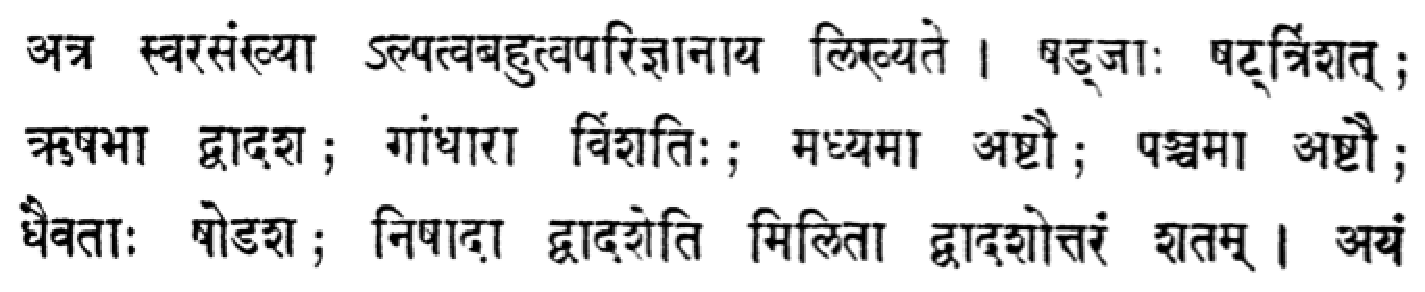
\includegraphics[scale=.35]{figures/5.eps}
\caption{Frequencies of \textsl{svara}-s in a particular \textsl{rāga}}\label{chap3-fig3}
\end{figure}

\newpage

“let us write down the infrequent or copious nature of the \textsl{svara}-s”\index{svara@\textsl{svara}} in the \textsl{rāga}\index{raga@\textsl{rāga}} and lists \textsl{sa} as 36 times, \textsl{ri} 12, \textsl{ga} 20, \textsl{ma} 8, \textsl{pa} 8, \textsl{dha} 16, \textsl{ni} 12, times out of a total of 112 \textsl{svara}-s. 

Given that Bhāskara\index{Bhaskara@Bhāskara}\index{Multinomial Theorem} had already written down multinomial theorem c.1150 C.E., it is not clear if anyone took the next step of using a device such as (informally at least) a multinomial distribution\endnote{it models the probability of the total count after rolling a k-sided dice n times; here k is related to the number of different types of \textsl{svara}-s\index{svara@\textsl{svara}} that can be used in a given \textsl{rāga} and n the length of the non-\textsl{sāhitya} part under discussion.} to generate the \textsl{svara}-s as a first small step!

An even more sophisticated but related model is available in an outline from Ānandavardhana\index{Anandavardhana@Ānandavardhana} based on Bhartṛhari's\index{Bhartrhari@Bhartṛhari} insights. Here, \textsl{sphoṭa}\index{sphota@\textsl{sphoṭa}} is the suggester and \textsl{dhvani}\index{dhvani@\textsl{dhvani}} the suggestion with \textsl{dhvani} elaborating \textsl{sphoṭa}. Using an aural point of view, \textsl{Sphoṭa} is said to arise from \textsl{sparśa} (contact), and produces a succession of sound waves, the \textsl{dhvani}, which is aurally perceptible. Just as there can be echoes for a well struck sound reaching us in a temporal sequence, there can be “echoes” of meaning at various levels, revealing the meaning sequentially (for example, \textsl{krameṇa pratibhāty ātmā yo 'syānusvāna-sannibhaḥ} in \textsl{Dhvanyāloka} 2.20). . For example, Sreenivasa Rao (2017) says:
\begin{figure}[H]
\centering
\includegraphics[scale=.5]{figures/6.eps}
\caption{Traces of \textsl{svara}-s of a \textsl{rāga}\index{raga@\textsl{rāga}}}\label{chap3-fig4}
\end{figure}

\begin{myquote}
The approach adopted by Bhartṛhari in explaining the process of true cognition is significantly different from that of the other Schools. Bhartṛhari argues that perception need not always be an ‘all–or-nothing process’. It could very well be a graded one. There could be vagueness initially; but, the perception could improve as one tries to gain clarity of the object. That is to say; the process of revelation could start from the indeterminate stage and progress, in steps, to the determinate stage. At each successive step, it gains increasing clarity. It begins from complete ignorance, passes through partial knowledge and ends up in a complete knowledge.

Thus, the position of Bhartṛhari is that the overcoming of error is a perceptual process by progressing through degrees of positive approximations. Even invalid cognitions can sometimes lead to valid knowledge (say, as in trial-and-error). Initial errors or vagueness could gradually and positively be overcome by an increasingly clearer cognition of the word form or \textsl{Sphoṭa}. That is to say; the true cognition, established by direct perception, could take place, initially, through a series of possible errors; but, finally leading to the truth.
\end{myquote}

Bhartṛhari\index{Bhartrhari@Bhartṛhari} and Ānandavardhana are arguing for what is now called a “Bayesian model”\index{Bayesian model}\index{Model types!Bayesian model} for the evolution of “meaning”. In the initial stages, the meaning is the “prior” given by the \textsl{abhidhā}\index{abhidha@\textsl{abhidhā}}\index{Aspects of meaning!abhidha@\textsl{abhidhā}} of the \textsl{pada}-s; as other information trickles in, the meaning changes with an associated probability distribution. The background, \textsl{kāla}, \textsl{deśa}, etc. of the hearer or the experiences (\textsl{anubhava})\index{anubhava@\textsl{anubhava}} of the \textsl{sahṛdaya}\index{sahrdaya@\textsl{sahṛdaya}} decides the specific distribution finally used. 

A mathematical structure with a probabilistic generative model\index{probabilistic generative model}\index{Model types!Latent Dirichlet Allocation (LDA)} such as a “Latent Dirichlet Allocation” (\textbf{LDA}), also called “graphical models”, may be needed as a starting point (as it is only a “bag-of-words” model, and \textsl{ārohaṇa}\index{arohana@\textsl{ārohaṇa}} and \textsl{avarohaṇa},\index{avarohana@\textsl{avarohaṇa}} for example, cannot be handled directly) and interestingly, research literature supports this view, at least in the \textsl{rāga}\index{raga@\textsl{rāga}} domain. Here, \textsl{svara}-s\index{svara@\textsl{svara}} are like words, musical phrases (e.g., \textsl{sañcāra}-s\index{sancaras@\textsl{sañcāra}-s} in Karnatic\index{Karnatic music}\index{Indian Classical Music!Karnatic} or \textsl{pakaḍ}-s\index{pakads@\textsl{pakaḍ}-s} in Hindustani\index{Hindustani music}\index{Indian Classical Music!Hindustani} music) like sentences, and \textsl{rāga}-s\index{raga@\textsl{rāga}} topics\endnote{Extensions can be attempted, possibly with just a different set of constants in the generative models for some, but more details for others, for structures such as \textsl{pallavi, anu-pallavi, chiṭṭa-svaram, muktāyi-svaram, caraṇam, rāga-mālikā-}s, \textsl{kīrtana}-s, etc.}. Furthermore, each \textsl{gamaka}\index{gamaka@\textsl{gamaka}} (ornamentation) can be seen to be a time series but distributed in a range of adjacent \hbox{\textsl{svara}-s}. Recent research in machine learning has shown how some context sensitive aspects can be attempted to be included in extended LDA-based models. In the case of \textsl{Rasa} Theory,\index{Rasa Theory@\textsl{Rasa} Theory} a model would have to incorporate how \textsl{bhava}-s are characterized as \textsl{sthāyi},\index{sthayibhava@\textsl{sthāyibhāva}} \textsl{sañcāri-/vyabhicari-},\index{sancaribhava@\textsl{sañcāribhāva}}\index{vyabhicaribhava@\textsl{vyabhicāribhāva}} and \textsl{sāttvika},\index{sattvikabhava@\textsl{sāttvikabhāva}} as well as how \textsl{ālambana}/\textsl{uddīpana vibhāva}-s\index{vibhava@\textsl{vibhāva}} produce the \textsl{bhāva}-s\index{bhava@\textsl{bhāva}} that finally become \textsl{anubhāva}-s.\index{anubhava@\textsl{anubhāva}}
 Given the extensive and detailed psychosomatic modelling in texts like \textsl{Nāṭyaśāstra},\index{Natyasastra@\textsl{Nāṭyaśāstra}} it is not easy to come up with good validated models that correspond to the insights therein. We however believe such a modelling perspective is possible, using some approximations, across many \textsl{kalā}-s\index{kala@\textsl{kalā}} using more detailed graphical models. Interestingly, in the domain of art and sculpture, VS Ramachandran\index{Ramachandran, V. S.} and Hirstein have theorized about a “peak shift” for understanding the stylized portrayal of human (female) forms which, though anatomically difficult, are aesthetically pleasing (Ramachandran 1999); this may be seen, in a basic model, as a change in the constants in a generative model\endnote{Furthermore, there could be a meaningful “quantum neural computing” model as (Kak\index{Kak, Subhash} 2008) has argued but we will not pursue it here.}.

A composer of an art form uses a sequence of atoms (\textsl{svara}-s,\index{svara@\textsl{svara}} \hbox{\textsl{mudrā}-s},\index{mudra@\textsl{mudrā}} \textsl{gaṇa}-s,\index{gana@\textsl{gaṇa}} etc) to express some \textsl{bhāva}/\textsl{rasa}.\index{bhava@\textsl{bhāva}}\index{rasa@\textsl{rasa}} It is likely that, across art forms, only a few limited \textsl{bhāva}-s are available, but with \textsl{sahṛdaya}-s\index{sahrdaya@\textsl{sahṛdaya}} it can be large. The mapping, too, is not completely definable (as per Bhartṛhari’s\index{Bhartrhari@Bhartṛhari} paradoxes). The actor (or the director) has to understand what these sequences of atomic units mean, or are perceived to be; or it could even be indeterminate (just as with a series of \textsl{svara}-s). It is possible that there are multiple meanings, and the actor has to emote a suitable one, or leave it open ended (as in the case of the meaning of \textsl{svara}-s in a musical phrase).

Now supposing that we understand the basic units of each art form, the next step is to help understand \textsl{bhāva}/\textsl{rasa} as a phenomenon in the context of a composer, an enactor and a \textsl{rasika}/audience. It is clear that there is some element of simulation (vide Śaṅkuka\index{Sankuka@Śaṅkuka} and keeping also views of other thinkers against this perspective); neurologically, the mirror neurons\endnote{There are some nerve cells (“mirror neurons”)\index{mirror neurons} in the frontal lobes thought to be involved in the production of complex movements but which also fire when the animal perceives the same movements performed by an experimenter (Pellegrino 1992).} are likely to be implicated. There seems to be also a large mirror neuronal complex that seems to be at work with respect to enactment and spectating --- just as in the AG (Attribute Grammar) formalism of synthesized and inherited attributes, neuronal outputs can be synthesized or inherited!

The second part is the communication itself through an actor, reader, music performer, etc. The theoretical question here is whether these intermediaries experience the \textsl{rasa}s themselves! Whether these are real or virtual? Some of the questions are: does the enactor feel the \textsl{rasa}, or does only the \textsl{rasika} feel it? Abhinavagupta\index{Abhinavagupta} argued for the former, while later scholars such as Rūpa\index{Rupa Gosvamin@Rūpa Gosvāmin} Gosvāmin did for the latter. Again, from a neuroscience perspective, depending on the inhibitor circuits with respect to mirror neuronal complex, both seem in principle feasible (just as Bharata\index{Bharatamuni} left both possibilities open).

The effect of some sequence of atomic units can be postulated as a combination of a cognitive state + affective state. Affective states are not cognitive, hence more likely related to non-representational aspects in the nervous system, especially evolved for quick involuntary responses such as “fight or flight” responses (mediated by the sympathetic nervous system) or “feed and breed” responses when body is at rest (mediated by the parasympathetic nervous system) but these are whole-body responses (unlike “local” inflammations or infections).\break With respect to \textsl{rasa},\index{rasa@\textsl{rasa}} the parasympathetic system is likely to be more pertinent. 

To proceed further, we postulate a plausible neurobiological model here; our model is not dissimilar to more detailed models in neuroscience research literature (for example, Roger Orpwood’s\index{Orpwood, Roger} theory discussed earlier). To aid in a quick emotional response, neurotransmitters (such as acetylcholine in the parasympathetic system) or other neuro-chemicals are generated by the nervous system that in turn is accepted by various types of receptors present in various organs such as the heart, stomach, etc, for producing an affective physical response. Since the number of such neuro-chemicals combinations are limited (contrast with the extremely large number of self and alien molecules to be recognized in the immunity system (in billions) and the corresponding matching molecules to be produced), one can postulate that the \textsl{bhāva}-s\index{bhava@\textsl{bhāva}} generated, even if many, are most likely common across art forms. 

If only sub-critical sets or quantities of neurotransmitters/neuro\-chemicals are produced, there will be no clearly identifiable state. If \textsl{bhāva}-s are sustained repeatedly (“\textsl{sthāyi}”),\index{sthayibhava@\textsl{sthāyibhāva}} a specific \textsl{rasa}\index{rasa@\textsl{rasa}} will result (connections with Orpwood’s\index{Orpwood, Roger} theory for \textsl{qualia}\index{qualia@\textsl{qualia}} can be recalled here). Initially, the \textsl{rasa} response can be said to be very dependent on \textsl{vibhāva}-s,\index{vibhava@\textsl{vibhāva}} but if positive feedback loops are present, the response can become independent of the initial excitation. Depending on the specific components of the \textsl{bhāva}-s, different \textsl{rasa}-s may be possible. Furthermore, given the \textsl{anubhāva}-s\index{anubhava@\textsl{anubhāva}} in the model, we have a Bayesian\index{Bayesian model}\index{Model types!Bayesian model} model, possibly a mixture model.

These \textsl{bhāva}-s, though in principle infinite in number as Bharata\index{Bharatamuni} mentions, only a few “high level” \textsl{bhāva}-s are learnable in any cultural setting and this could be a differentiating marker across cultures. Interesting questions that arise are: Can we show that the \hbox{\textsl{bhāva}-s}\index{bhava@\textsl{bhāva}} produced in music are the “same” as those produced in drama, poetry, etc., especially in a neuroscience perspective? That is, are the connectome excitation patterns\index{patterns!excitation} the same across the brain?

Are all the art forms potent in producing all the \textsl{bhāva}-s? While this seems to be unlikely (for example, consider \textsl{tālavādya}-s\index{talavadya@\textsl{tālavādya}} such as \textsl{mṛdaṅga}\index{mrdanga@\textsl{mṛdaṅga}} or even simpler non-tonal ones), one can pose a Turing-like question: Is there a universality notion (ie. is the art form complete in some sense)? Similarly, is there a mapping, say, of some \hbox{\textsl{svara}-s}\index{svara@\textsl{svara}} to \textsl{mudrā}-s?\index{mudra@\textsl{mudrā}} We have already mentioned the mapping between colour and \textsl{bhāva}/emotions earlier in the \textsl{Viṣṇudharmottara}\index{Visnudharmottarapurana@\textsl{Viṣṇudharmottara Purāṇa}} (and this phenomenon is also known through synaesthetes). Some studies have shown that a sudden transition from low to high pitch often indicates pathos across many cultures; however, while some gestures may be common across cultures, there may be some with possibly opposite semantics!

Another question is whether “\textsl{rasa}” is accessible to all. While there are many possible responses to this question, the Indic tradition affirms it with respect to \textsl{bhakti rasa}.\index{rasa@\textsl{rasa}!bhakti@\textsl{bhakti}}\index{bhaktirasa@\textsl{bhakti-rasa}}  In his development of \textsl{bhakti rasa}, Rūpa\index{Rupa Gosvamin@Rūpa Gosvāmin} Gosvāmin says that enjoying \textsl{rasa nitya} is possible if one views life in terms of drama, using the language of \textsl{rasa}\index{rasa@\textsl{rasa}} and redirecting it toward the development and expression of \textsl{bhakti}.

Going by our brief discussion of Bhartṛhari’s\index{Bhartrhari@Bhartṛhari} paradox, it should be clear that the mapping from a specific enactment of an art form to the \textsl{rasa} in general is “non-computable”; ie. it is not clear \textsl{a priori} what output is to be expected for a particular event. This is where different civilizational impulses can be seen: \textsl{mano-dharma}\index{manodharma@\textsl{mano-dharma}} in the Indic case but realism or carefully constructed “scores” that had to be reproduced precisely and accurately in the European one. 

\subsection{A Computer Systems Model for Communication Across Multiple Roles and Multiple Persons}\label{chap3-sec4.2}

This section can be skipped by those who are not exposed to computer systems notions of virtual machines and the like. In computer science, we have the notion of a “virtual” machine\index{Virtual machine} (\textbf{VM}) that is emulated or simulated by a more “physical” machine, as there can be many levels at which this emulation or simulation notion can happen. The inputs and outputs of these virtual machines can be demultiplexed or multiplexed as necessary.

In an art form, there is the self of the spectator/reader (\textbf{“3S”}), the self of the composer/creator (\textbf{“1S”}) and the self of the enactor” (\textbf{“2S”}); the 1,2,3 refer to first person, 2nd person and 3rd person respectively with S standing for the self. Let us take a simpler case first. Crucially, the ability to empathise with someone depends on a person (“1S”) being able to imagine the state of someone else (“3S”); if there is considerable depth of feeling, there could be corresponding changes in the emotional state also. For this to happen, it is critical that both the self of the person (“1S”) and that of the sympathised (“3S”) be operative at the “same” time (or “timeshared” frequently enough, from a scheduling point of view). In a computational sense, one can imagine a type-II virtualization scheme where the “1S” machine, \textbf{1SM}, runs a new virtual machine\index{Virtual machine} for the “3S” machine, \textbf{3SM}, and sets it up in such a way that some of the inputs to 1SM, “seized” as necessary, are “tunnelled” to 3SM. The outputs of the 3SM virtual machine have to be carefully steered; if the outputs are “tunnelled” out of the 1SM then we have perfect isolation between 1SM and 3SM. But tunnelled out to whom or where to? There could be some output devices “seized” by 3SM. In which case, the drivers of 1SM will be used for output to these devices. Or, alternatively, 3SM delegates the output function to 1SM system, and 1SM simulates the output function.

If this is not possible to answer, one solution is for the 1SM to directly indicate the output (ie. use 1SM’s drivers to communicate with the external world). But this means that 1SM cannot indicate externally the state of 3SM. 

Some of the questions posed in the Indic tradition:
\begin{itemize}
\itemsep=0pt
\item[(i)] Can the enactor feel the \textsl{rasa}?\index{rasa@\textsl{rasa}} If the outputs of the VM\index{Virtual machine} are tunnelled out or faithfully emulated, then the enactor (“2S”) need not sense anything. Otherwise, one can argue that there will be some “leakage” of the \textsl{rasa} into the enactor. Abhinavagupta\index{Abhinavagupta} argues for the first case. However, it is well known that leakage of state from one VM to another is possible due to non-virtualizable features (“sensitive instructions”) or due to non-isolation from a performance perspective. 

\item[(v)] Since we are dealing with a CPS, and the enactor (“2S”) has to signal the emotions through \textsl{mudrā}-s\index{mudra@\textsl{mudrā}} and the like, the outputs of the 3SM have to be again transcoded and presented to the audience through the 1SM’s physical gestures. Here it can be \textsl{lokadharmin}\endnote{\textsl{Loka-dharmin} is realistic with a natural presentation of the world (similar to current movies) catering to the “common man”, whereas \textsl{nāṭya-dharmin}, or stylized drama, uses gesture language and symbols, and more artistic but for \textsl{sahṛdaya}-s.\index{sahrdaya@\textsl{sahṛdaya}}} or \textsl{nāṭyadharmin}. The first one is suitable for a general audience but the latter most likely only for \textsl{sahṛdaya}-s.\index{sahrdaya@\textsl{sahṛdaya}}

\newpage

\item[(vi)] Should the identification of the enactor and the character be complete for “realism”? In the Indic tradition, the attempt is not so much at realism as to bring out the \textsl{rasa}. The attempt is more to trigger the desired cognitive/affective states in the \hbox{\textsl{sahṛdaya}-s} symbolically through \textsl{mudrā}-s\index{mudra@\textsl{mudrā}} and the like. Hence the gestures are stylized and the grammar of gestures generates the desired states.

\item[(vii)] Can the self be “unitary”? This problem is similar to the issues in the sleep states in the Indic tradition. Vedānta postulates a basal self across the sleep states to answer the question why we “know” that we slept deeply but at the same time we “did not know anything” during that time. Here, we have multiple VMs\index{Virtual machine} and therefore the basal self (or the “host OS”) is responsible for switching between various emotions or even across multiple characters.
\end{itemize}

There is also an interesting problem in the context of a CPS + \textsl{rasa}:\index{rasa@\textsl{rasa}} do we need in general a self-reproducing machine? Note that each emulated living entity will have a corporeal aspect that has to be used to communicate interactions with the real world; this means, the simulated VM\index{Virtual machine} needs to have a physical body too (for eg, an elephant, bird, \textsl{devi}, etc) and realized at run time. In the most general case, given the person/living entity to be conveyed, we need the physical emulation/realization using the body of the enactor. For ease, many \textsl{mudrā}-s\index{mudra@\textsl{mudrā}} have been instead developed to represent the various entities (e.g., parrots).\\[-20pt]

\subsection{\textsl{Rasa} in Music: an Example}\label{chap3-sec4.3}

Let us consider music first. We first discuss the cognitive part. In the earliest phase, Vedic chanting in \textsl{Sāma Veda}\index{Samaveda@\textsl{Sāmaveda}}\index{Veda-s@\textsl{Veda}-s!Samaveda@\textsl{Sāmaveda}} used 3 \textsl{svara}-s\index{svara@\textsl{svara}} and it was extended later in music to 5, 7, 12, 22, ... \textsl{svara}-s; these numbers Kak\index{Kak, Subhash} points out, may be related to Meru\index{Meru Prastara@Meru Prastāra}-prastāra. There were obviously deep connections with \textsl{chandas}/poetry\index{chandas@\textsl{chandas}} and redundancy/checksums as anti-entropy measures with various styles of chanting such as \textsl{pada},\index{padapatha@\textsl{pada-pāṭha}}\index{Vedic chanting, \textsl{vikṛti-pāṭha}-s!krama@\textsl{krama}}\index{Vedic chanting, \textsl{vikṛti-pāṭha}-s!ghana@\textsl{ghana}}\index{Vedic chanting, \textsl{vikṛti-pāṭha}-s!ratha@\textsl{ratha}}\index{Vedic chanting, \textsl{vikṛti-pāṭha}-s!danda@\textsl{daṇḍa}}\index{Vedic chanting, \textsl{vikṛti-pāṭha}-s!dhvaja@\textsl{dhvaja}}\index{Vedic chanting, \textsl{vikṛti-pāṭha}-s!jata@\textsl{jaṭā}}\index{Vedic chanting, \textsl{vikṛti-pāṭha}-s!mala@\textsl{mālā}}\index{Vedic chanting, \textsl{vikṛti-pāṭha}-s!rekha@\textsl{rekhā}}\index{Vedic chanting, \textsl{vikṛti-pāṭha}-s!sikha@\textsl{śikhā}}\index{ghanapatha@\textsl{ghana-pāṭha}} \textsl{krama}, \textsl{jaṭā}, \textsl{mālā, śikhā, rekhā, dhvaja, danda, ratha, ghana}. Phonological combinations (\textsl{sandhi}) have been devised taking into account what is realizable given our human anatomy with respect to speech; they result in lesser effort and so can be said to be euphonic. If iterative or recursive structures are devised, “vibrational” sensations can in principle be auditorily excited. Historically, for example, Mataṅga\index{Matanga@Mataṅga} discusses \textsl{Ṣaḍja-grāma} and \textsl{Madhyama-grāma} as two basic \textsl{Grāma}-s (groups or clusters); \textsl{grāma}-s are collection of \textsl{svara}-s in consecutive order. From these arise \textsl{mūrcchanā}, \textsl{tāna}, \textsl{jāti} and \textsl{rāga}.\index{raga@\textsl{rāga}} \textsl{Mūrchānā}-s are a set of systematic rotations of the \textsl{saptaka} with an \textsl{ārohaṇa}\index{arohana@\textsl{ārohaṇa}} and \textsl{avarohaṇa}\index{avarohana@\textsl{avarohaṇa}}
 (so 7 for each \textsl{grāma}). These are described by Bharata\index{Bharatamuni} earlier also but something deeper in structure was felt to be needed; this sense later resulted in the innovation of the \textsl{rāga} paradigm\endnote{We can take as an example a \textsl{rāga} that falls in the ``\textsl{adbhuta-rasa}"\index{adbhuta@\textsl{adbhuta}}\index{rasa@\textsl{rasa}!adbhuta@\textsl{adbhuta}}   (wonderment and awe) of the \textsl{nava-rasa-}s\index{navarasa@\textsl{nava-rasa}} (nine emotions). Kumudakriyā, the \textsl{janya rāga}\index{raga@\textsl{rāga}!janya@\textsl{janya}}\index{janyaraga@\textsl{janya-rāga}} of Pantuvarāli (Kāmavardhinī), 51st \textsl{melakarta}, has been chosen by Muthuswami Dikshithar for his composition, “\textsl{Ardhanārīśvaram}”. See \url{https://www.youtube.com/watch?v=b5yuBGJugFw} (Kuldeep Pai) or \url{https://www.youtube.com/watch?v=E1HA1XPFT-M} (Aruna Sairam) [Accessed on 3rd January 2018]. The scale of Kumudakriyā-Ascending is Sa Ri Ga Ma Dha Sa with descending being Sa Ni Dha Ma Ga Ri Sa... A \textsl{rasika} comments “Contemplation on the \textsl{prayoga}-s or phrases Sa Ni Dha Ri', Ri Ga Ma Dha Ri, etc. invoke a sense of fantasy, make-believe or illusion. Imagine suddenly walking into somebody who is split into a perfect half of a perfect man and a perfect woman! ... Absolutely dazzling and surreal! Kumudakriyā, a breathtaking \textsl{rāga} of fantasy, ...”}. From iterative structures, the musical ideas turned to probabilistic ones\endnote{See also, e.g., (Rowell\index{Rowell, Lewis} 1992), for a comparable explanation: “What does this tell us about the relationship between theory and practice? A hallmark of the early Indian way of thinking about music was to identify and name all possible permutations of the basic elements, but with the realization that only certain authorized (and far more specific) melodic constructions can become the basis for actualized music, as, for example, in the form of an individual \textsl{rāga}. It was the job of the theory to provide the widest selection of possibilities, but it remained for practice to select the most pleasing of these arrangements. There is a reason for this: any purely mechanical set of permutations of a given system (of which the diatonic scale is an excellent example) will sooner or later exhaust the available possibilities and will admit no others. Such an outcome would violate a basic assumption of Indian culture, namely, that the number of available forms is, at least in theory, unlimited. The solution, which is as valid today as it was two thousand years ago, was to achieve the richness and profusion of forms that Indians demanded in their music by means of a musical system that could not be confined to any set of exclusive possibilities. On the contrary, they sought to devise a system that could accommodate any number of later additions, a system that was inclusive rather than exclusive. What the \textsl{mūrchana}-s and their derivatives provided was the simple notion that different octave segments (the \textsl{mūrchana}-s)\index{murchana@\textsl{mūrchana}} and certain of their subsets (the \hbox{\textsl{tāna}-s}) could, when colored by the emphasis or understatement of certain tones, and also by distinctive ornaments and melodic pathways- form the structural basis for a unique melodic construction: a \textsl{jāti}, a \textsl{grāma rāga}, or a \textsl{rāga}.”\index{raga@\textsl{rāga}}}.

A simplistic description for a \textsl{rāga}\index{raga@\textsl{rāga}} is as follows: choose an alphabet of \textsl{svara}-s,\index{svara@\textsl{svara}} use well established \textsl{sañcāra}-s\index{sancaras@\textsl{sañcāra}-s} or \textsl{prayoga}-s\index{prayogas@\textsl{prayoga}-s} (“signatures”) of the \textsl{rāga},\index{raga@\textsl{rāga}} and follow rules of \textsl{ārohaṇa} and \textsl{avarohaṇa} to generate yet more possible strings of \textsl{svara}-s as music. In actuality, there are many more critical features such as \textsl{aṁśa} (prominent or \textsl{jīva svara}-s), \textsl{alpatva} (\textsl{svara}-s that need to be present fewer in number), \textsl{bahulatva} (copious), \textsl{ṣāḍava/auḍava}: 6 note/5 note \textsl{sañcāra}-s, \textsl{antara mārga}: the introduction of note or \textsl{chāyā} of another \textsl{rāga}. Furthermore, only when the "\textsl{jīva svara}-s” are rightly used, we can induce life into a \textsl{rāga}.

RN Iyengar has suggested that a \textsl{rāga}\index{raga@\textsl{rāga}} is actually a \textsl{svara}\index{svara@\textsl{svara}} time series, evolving in the space of \textsl{ārohaṇa-avarohaṇa}\index{arohana@\textsl{ārohaṇa}}\index{avarohana@\textsl{avarohaṇa}} (scale) with the property of ‘\textsl{alpatva-bahulatva}’ (Iyengar 2017).\index{Iyengar, R. N.} Furthermore, “The scale can be nearly equated with the sample space of Probability Theory”. He also points out that Śārṅgadeva\index{Sarngadeva@Śārṅgadeva} actually gives many traces (sequences) of \textsl{svara}-s\index{svara@\textsl{svara}} for one \textsl{rāga} as an illustration; this has been discussed earlier.

Fundamentally, a \textsl{rāga}\index{raga@\textsl{rāga}} is not a static concept (due to notion of \textsl{manodharma\index{manodharma@\textsl{manodharma}}-saṅgīta}) and has a stochastic aspect. Iyengar and others have pointed out that the time series of \textsl{svara}-s can be modelled as a AR(1) process (\textbf{AR}: autoregressive (stochastic) process) with the following 1st order simple model: $\Phi(n) = k*\Phi(n-1)+$ noise, where $\Phi(n)$ is the \textsl{svara} at time unit $n$ and $k$ is a constant; many simple songs taught to beginners (“\textsl{pillāri gītam-}s”) have been shown to have this AR(1) property! More complex songs need many more terms as a AR(p) process that depends not only on on the $(n-1)$ instant, but on $(n-2),\ldots (n-p)$ instants. These can be shown experimentally by computing autocorrelation functions (\textbf{ACF}).

Furthermore, Iyengar says that the ACF of a \textsl{varṇam} has a fractal-like\index{fractals} structure and he conjectures that \textsl{kīrtana}-s in any \textsl{rāga}\index{raga@\textsl{rāga}} will be a more complex time series, exhibiting finer self similar structures embedded in the sample space. He posits that \textsl{rāga ālāpana} is actually a chaotic process with the \textsl{ārohaṇa-avarohaṇa}\index{arohana@\textsl{ārohaṇa}}\index{avarohana@\textsl{avarohaṇa}} providing the boundary of the “strange attractor”. As all of this is heard and experienced, \textsl{rāga} can be said to be a mathematically based stochastic process that generates \textsl{rasa}!\index{rasa@\textsl{rasa}}

In addition, using machine learning algorithms that use generative models (such as “LDA”), some researchers have shown higher rates of correct classification of \textsl{rāga}-s.\index{raga@\textsl{rāga}} (Of course, other models like “profile” HMMs\index{Hidden Markov Model (HMM)} (\textbf{pHMM}) could also be profitably explored; a pHMM has a profile that could apply to the parent \textsl{rāga} with \textsl{janya rāga}-s\index{raga@\textsl{rāga}!janya@\textsl{janya}} 
\index{janyaraga@\textsl{janya-rāga}}  being generated using the pHMM structures). These also imply deep down that a \textsl{rāga} has a substantial and inescapable stochastic structure that also can be discerned but which is sufficiently mathematically tractable. This is historically interesting: almost one millennium earlier, there has been the groundbreaking generative model of Pāṇini\index{Panini@Pāṇini} in his \textsl{Aṣṭādhyāyī}\index{Astadhyayi@\textsl{Aṣṭādhyāyī}} except that stochastic processes do not play a role in his system and his grammar is closer to a term writing system such as the Post Correspondence system formalized mathematically in 1920’s. For \textsl{rāga}-s,\index{raga@\textsl{rāga}} we also have a generative system but with a probabilistic core!


Next to briefly discuss the affective aspect of Indic music, the word \textsl{rāga}\index{raga@\textsl{rāga}} itself is defined as “\textsl{rañjayati iti rāgaḥ}”. There have been attempts at theorization at 2 levels of structure: at the level of \textsl{svara}-s\index{svara@\textsl{svara}} and at the level of \textsl{rāga}-s themselves. \textsl{Viṣṇudharmottara-purāṇa}\index{Visnudharmottarapurana@\textsl{Viṣṇudharmottara Purāṇa}} (III.18, \hbox{2--3}) gives the following scheme: “for \textsl{hāsya}\index{hasya@\textsl{hāsya}}\index{rasa@\textsl{rasa}!hasya@\textsl{hāsya}} and \textsl{śṛṅgāra, madhyama and pañcama} are used; for \textsl{vīra,\index{vira@\textsl{vīra}}\index{rasa@\textsl{rasa}!vira@\textsl{vīra}} raudra}\index{raudra@\textsl{raudra}}\index{rasa@\textsl{rasa}!raudra@\textsl{raudra}} and \textsl{adbhuta,\index{adbhuta@\textsl{adbhuta}}\index{rasa@\textsl{rasa}!adbhuta@\textsl{adbhuta}} ṣaḍja} and \textsl{ṛṣabha} are used; for \textsl{karuṇa,\index{karuna@\textsl{karuṇa}}\index{rasa@\textsl{rasa}!karuna@\textsl{karuṇa}} niṣāda} and \textsl{gāndhāra} are used; for \textsl{bībhatsa}\index{bibhatsa@\textsl{bībhatsa}}\index{rasa@\textsl{rasa}!bibhatsa@\textsl{bībhatsa}} and \textsl{bhayānaka,\index{bhayanaka@\textsl{bhayānaka}}\index{rasa@\textsl{rasa}!bhayanaka@\textsl{bhayānaka}} dhaivata} is used and for \textsl{śānta, madhyama} is used. Similarly for different \textsl{rasas} different \textsl{laya}-s\index{laya@\textsl{laya}} are used.” (Trans. Priyabala Shah). Some theorists assign \textsl{rasa} or \textsl{bhāva} to \textsl{rāga}-s on the basis of their \textsl{vādi} (dominant note) in the following way: infinity or space if the \textsl{vādi} is \textsl{sa}; illumination if the \textsl{vādi} is \textsl{ri}; devotion if the \textsl{vādi} is \textsl{ga}; erotic if the \textsl{vādi} is \textsl{ma}; joy or contentment if the \textsl{vādi} is \textsl{pa}; valour and disgust if the \textsl{vādi} is \textsl{dha}; and encouragement if the \textsl{vādi} is \textsl{ni}\endnote{Discussed interestingly in the CBSE class XI Music text (Kapoor and Danino 2012).}. Alternatively, \textsl{pa} (\textsl{pañcama}) is said to be for \textsl{śṛṅgāra};\index{srngara@\textsl{śṛṅgāra}}\index{rasa@\textsl{rasa}!srngara@\textsl{śṛṅgāra}} for example, \textsl{Gītagovinda}\index{Gitagovinda@\textsl{Gītagovinda}} 1.39 refers to a song being sung in \textsl{pañcama rāga}\index{raga@\textsl{rāga}} to evoke \textsl{śṛṅgāra}.

There is a long tradition in assigning \textsl{rāga}-s\index{raga@\textsl{rāga}} for evoking emotions in Hindustani\index{Hindustani music}\index{Indian Classical Music!Hindustani} and Karnatic\index{Karnatic music}\index{Indian Classical Music!Karnatic} systems. For example, \textsl{Śubhapantuvarāli} is said to indicate penitential emotions whereas \textsl{Aṭhāna} that of \textsl{vīra\index{vira@\textsl{vīra}}\index{rasa@\textsl{rasa}!vira@\textsl{vīra}} rasa}\index{rasa@\textsl{rasa}} and so on. Starting with probabilistic emphasis on the \textsl{vādi}\index{vivadi@\textsl{vivādi}} notes, specific \textsl{rāga}-s\index{raga@\textsl{rāga}} also indicate the emotions using musical phrases observing \textsl{ārohaṇa}\index{arohana@\textsl{ārohaṇa}} and \textsl{avarohaṇa},\index{avarohana@\textsl{avarohaṇa}} with specific phrases (the \textsl{sañcāra}-s\index{sancaras@\textsl{sañcāra}-s}/\textsl{pakaḍ}-s\index{pakads@\textsl{pakaḍ}-s} in Karnatic/Hindustani music, for example) being the signatures. Since there is no written score, each phrase can be elaborated multiple times possibly with different ornamentation; there is thus probabilistic emphasis on different phrases as well as ornamentation (“\textsl{gamaka}”)\index{gamaka@\textsl{gamaka}} giving rise to a richly textured music that can evoke deep emotions. Even \textsl{tāla}-s\index{tala@\textsl{tāla}} are expected to contribute to the \textsl{rasa}; for example, \textsl{pratimaṇṭha tāla} is said to enhance \textsl{śṛṅgāra}\index{srngara@\textsl{śṛṅgāra}}\index{rasa@\textsl{rasa}!srngara@\textsl{śṛṅgāra}} (Narayanan 2016). 

The Indic seers (take, for example, Abhinavagupta)\index{Abhinavagupta} intuited music’s capacity to help us approach the transcendental plane and this has been borne by recent studies; for example, Janata and others, as discussed before, have identified the temporo-parietal junction (TPJ) region that is the location of self-referential activity as the locus of music also. Music is a highly personal experience while making us also feel a part of the whole “universe” in an abstract way; interestingly, the notion of \textsl{sādhāranīkaraṇa}\index{sadharanikarana@\textsl{sādhāraṇīkaraṇa}} is useful in the latter as it posits universals across all.

\section{Computational Thinking and its Relevance for \textsl{Rasa}}\label{chap3-sec5}

While one running thread in Indian aesthetics or \textsl{rasa}\index{rasa@\textsl{rasa}} is the taxonomical approach, it was married, often enough, to a computational base. While the taxonomy part has been widely recognized (for example, the \textsl{vyabhicāribhāva},\index{vyabhicaribhava@\textsl{vyabhicāribhāva}} the transitory state of mind or body, said to be 34 in number such as \textsl{asūyā, nirveda, glāni, śaṅkā}\index{asuya@\textsl{asūyā}}\index{nirveda@\textsl{nirveda}}\index{glani@\textsl{glāni}}\index{sanka@\textsl{śaṅkā}} etc), the computational aspect has not been appreciated as much and one can say that this served possibly as a possibly unique or distinguishing part of the tradition. Furthermore, detailed psycho-physical (taxonomical) models in, for example, \textsl{Nāṭyaśāstra}\index{Natyasastra@\textsl{Nāṭyaśāstra}} are helpful in a computational model as we have discussed in \S\ref{chap3-sec4} for modelling emotions. We now give some examples of computational thinking and its relevance for \textsl{rasa} in a few art forms, mostly from a generative perspective; the interested reader can find some background on computational thinking and the specific Indic context as two appendixes (APPENDIX 1 and 2). Note that when we discuss \textsl{rasa} here it is, at a more general level and not only in the context of Bharata’s\index{Bharatamuni} formulation.\\[-20pt]

\subsection{The Computational Basis of \textsl{Rasa} in Poetry}\label{chap3-sec5.1}

The Veda-s\index{Veda-s@\textsl{Veda}-s} are alternately called “\textsl{chandas}", thus there is close connection between poetry and visions of reality (“\textsl{rtam}”). The study of poetry therefore assumed an important part of the intellectual tradition, for example, \textsl{Nirukta},\index{Nirukta@\textsl{Nirukta}} \textsl{śikṣā}, etc. Continuing in this tradition, Piṅgala\index{Pingala@Piṅgala} enumerated the number of \textsl{tāla}-s\index{tala@\textsl{tāla}} through cryptic \textsl{sūtra}-s in \textsl{Chandaḥ-śāstra}.\index{Chandahsastra@\textsl{Chandaḥ-śāstra}} The motivation doubtless was that if we need to understand music, it helps to know, if feasible, how many possibilities exist for a specific entity in a system that need to be examined individually for tractability or practicalness\endnote{See (Rowell\index{Rowell, Lewis} 1992) for a comparable explanation.}. The idea here may have been to possibly look at all possible ways of structuring syllables, long or short, given a specified amount of time and in the process invented Piṅgala sequence\index{Pingala sequence@Piṅgala sequence} (\textbf{P}), now inadvertently called Fibonacci\index{Fibonacci series} series (0,1,1,2,3,5,8,13,...)\endnote{Fibonacci\index{Fibonacci series} wrote a book, about 1202, that discussed Indian mathematics, translated into Syriac/Arabic, as the basis; the name for the series was given only in c. 1870's by Lucas who proved \verb|2^{127}-1| is prime using these numbers.}. Piṅgala\index{Pingala@Piṅgala}
 or his disciples also noted that in this sequence the next term is given by the sum of the 2 earlier terms (starting from the 3rd term). Elaborating explicitly (Knuth\index{Knuth, D. E.} 1997), Gopāla\index{Gopala@Gopāla (mathematician)} (before 1135 C.E.) and Hemacandra\index{Hemacandra} (around 1150 C.E.) give the number of \textsl{tāla} (rhythmic patterns)\index{patterns!rhythmic} for \textsl{\textbf{M}} \textsl{mātrā} (beats) (“P(\textsl{M})”) with \textsl{anudruta} (1-beat) and \textsl{druta} (2-beat) algorithmically as \textsl{tāla} (\textsl{M}) = \textsl{tāla} ($\text{\textsl{M}}-1$) + \textsl{tāla} ($\text{\textsl{M}}-2$), or P(\textsl{M}) = P($\text{\textsl{M}}-1$) + P($\text{\textsl{M}}-2$)\endnote{The recursive or iterative property of the series can be seen as follows by case analysis, as either an \textsl{anudruta} coming first or the \textsl{druta}. First fix an \textsl{anudruta} as the 1st in the sequence; the remaining ($\text{\textsl{M}}-1$) beats have P($\text{\textsl{M}}-1$) distinct possibilities. Next, fix a \textsl{druta} as the 1st in the sequence; the remaining ($\text{\textsl{M}}-2$) beats have P($\text{\textsl{M}}-2$) distinct possibilities. The sum therefore gives P(\textsl{M}).}.

Investigating \textsl{chandas}\index{chandas@\textsl{chandas}} further, the concept of \textsl{gaṇa}-s\index{gana@\textsl{gaṇa}} were introduced. These are groups of 3 syllables, \textsl{anudruta}/short/\textsl{laghu} (“U”) or \textsl{druta}/long/\textsl{guru}\index{anudruta@\textsl{anudruta}}\index{laghu@\textsl{laghu}}\index{druta@\textsl{druta}}\index{guru@\textsl{guru}} (“|”); hence 8 possible \textsl{gaṇa}-s (inaugurating the start of binary notation, now commonplace). From a coding perspective, each specific \textsl{gaṇa} can be considered as the “summary” or checksum/hash of 3 syllables\endnote{Interestingly, the process of coming up with a mnemonic for remembering the various \textsl{gaṇa}-s (“\textsl{yamātārājabhānasalagam}”) threw up the earliest known example of what has later been called memory wheels (first noted in 1880’s by those working on codes in telegraphy) or de Bruijn sequences\index{de Bruijn sequences} (1944) (see (Knuth\index{Knuth, D. E.} 2011)).} and hence the sequences of these summaries can be used as a way to detect corruption if the poetic structure is violated. These are described in Alaṅkāraśāstra, for example, the Śārdūlavikrīḍita with “msjsttg” structure, redolent of the forest as it recalls a tiger cub’s playfulness (with \textsl{virāma} in the 12th syllable and then another 7 syllables away). Since \textsl{alaṅkāra śāstra}\index{alankarasastra@Alaṅkāraśāstra} and its connection with \textsl{rasa}\index{rasa@\textsl{rasa}} has been discussed in the tradition widely, we focus on other aspects, specifically the computational as it relates to \textsl{rasa}. The choice of meters widely used could be connected with the locality principle we discussed in the context of music; the locality could be in terms of pitches\endnote{In Telugu, \textsl{prāsa} is also present to a considerable degree: for example, use of same consonant at fixed positions.} as the poem is recited or in terms of sequenced “chords” of \textsl{gaṇa}-s\index{gana@\textsl{gaṇa}} (but different from Western Music chords!)

Because \textsl{rasa} is now married to function, there is a robustness in the transmission of \textsl{śloka}-s written to various types of \textsl{chandas}\index{chandas@\textsl{chandas}} that is not possible in other traditions except in a rudimentary way. Advancing the robustness further, in the Vedic domain, the generative aspect interestingly has been further married to a functional notion, that of resistance to local decay or destruction (reliability in short) either when chanted orally or when written on fragile materials; this again depends on a computational basis. Chanting styles (\textsl{vikṛti}-s)\index{Vedic chanting, \textsl{vikṛti-pāṭha}-s}\index{vikrti@\textsl{vikṛti}} were invented that introduced controlled amounts of redundancy such as \textsl{krama, jaṭā, mālā, śikhā, rekhā, dhvaja, daṇḍa, ratha, ghana},\index{Vedic chanting, \textsl{vikṛti-pāṭha}-s!krama@\textsl{krama}}\index{Vedic chanting, \textsl{vikṛti-pāṭha}-s!ghana@\textsl{ghana}}\index{Vedic chanting, \textsl{vikṛti-pāṭha}-s!ratha@\textsl{ratha}}\index{Vedic chanting, \textsl{vikṛti-pāṭha}-s!danda@\textsl{daṇḍa}}\index{Vedic chanting, \textsl{vikṛti-pāṭha}-s!dhvaja@\textsl{dhvaja}}\index{Vedic chanting, \textsl{vikṛti-pāṭha}-s!jata@\textsl{jaṭā}}\index{Vedic chanting, \textsl{vikṛti-pāṭha}-s!mala@\textsl{mālā}}\index{Vedic chanting, \textsl{vikṛti-pāṭha}-s!rekha@\textsl{rekhā}}\index{Vedic chanting, \textsl{vikṛti-pāṭha}-s!sikha@\textsl{śikhā}} with the \textsl{ghana}\index{ghanapatha@\textsl{ghana-pāṭha}}\index{Vedic chanting, \textsl{vikṛti-pāṭha}-s!ghana@\textsl{ghana}} being the most complex (the sequence of syllables a1 a2 a3 a4, for example, being chanted, 3 syllables at a time but sliding with one syllable at a time, as a1 a2, a2 a1, a1 a2 a3, a3 a2 a1, a1 a2 a3; a2 a3, a3 a2, a2 a3 a4, a4 a3 a2, a2 a3 a4, an expansion by a factor of 11 with a corresponding increase in robustness with respect to local decay). The repetition in these codes has a hypnotic effect when chanted as those who have heard \textsl{ghana\index{ghanapatha@\textsl{ghana-pāṭha}}\index{Vedic chanting, \textsl{vikṛti-pāṭha}-s!ghana@\textsl{ghana}} pāṭha} can testify. The Indic imagination therefore approvingly quotes \textsl{āśrama}-s and such where such recitations would continue “nonstop”.

Kashyap and Bell have investigated the robustness of such chanting styles using coding theory and formulate \textsl{Krama-māla} style of chanting as a “rate 1/4 linear block code over a finite Galois field”; they show that with this code a text of 4n symbols can be corrected even with as many as 2(n-1) errors under some assumptions (Kashyap 1998). While requiring the preservation of the order of words, the errors to be detected are the add/delete of a syllable/word in a word/sentence or avoiding “long jumps”. To explain the latter, consider a set of syllables A (in verse x) that is similar to a set B (in verse y) and we are chanting of  ...AC... ; ...BD... Now we can mistakenly chant say ...AD... or ...BC..., ie “jump” across due to similarity between A and B. Specific styles of chanting such as \textsl{avichakra} \textsl{ratha} handle these by appropriate coding. Kashyap and Bell give the following interesting example as it involves the very first mantra in \textsl{Ṛgveda}:\index{Rgveda@\textsl{Ṛgveda}}\index{Veda-s@\textsl{Veda}-s!Rgveda@\textsl{Ṛgveda}}

\newpage

\begin{myquote}
\textsl{Ṛgveda} 1.1.1     ... C \textsl{ratnadhātamam} (A)

\textsl{Ṛgveda} 1.20.1    ... E \textsl{ratnadhātamaḥ} (B) D
\end{myquote}

\vskip .1cm

Chanting is coded so that A chained to C and B to E to prevent jump from C to B and E to A. If there is incorrect chanting, this code can point out the error. 

\vskip .1cm

Using such computational coding ideas, \textsl{Veda}-s\index{Veda-s@\textsl{Veda}-s} have been transmitted mostly orally across at least 3500-5000 years without differing versions but including exact pronunciation (with, it is said, only one doubtful reading in \textsl{Ṛgveda} at \textsl{Ṛgveda}\index{Rgveda@\textsl{Ṛgveda}}\index{Veda-s@\textsl{Veda}-s!Rgveda@\textsl{Ṛgveda}} 7.44.3 after a lapse of as much as 7000 years)! UNESCO proclaimed the tradition of Vedic chant a “Masterpiece of the Oral and Intangible Heritage of Humanity” on November 7, 2003. (Of course, such clever mathematical ideas cannot survive wholesale destructions of cultures that spawn them as happened with the Indic ones, especially in Kāśmīr.)

\vskip .1cm

Continuing in the same strain, surprise or wonder as a generative component of \textsl{rasa}\index{rasa@\textsl{rasa}} could be channelled computationally for linguistic problems that need techniques such as backtracking; e.g., Knight’s Tour\index{Knight’s Tour problem} problem considered by Rudraṭa\index{Rudrata@Rudraṭa} and also by Vedānta Deśika\index{Vedantadesika@Vedānta Deśika} and many others. The earliest known reference to the Knight's Tour problem called the \textsl{``turaga-pada-bandha''} dates back to the 9th century C.E. by Rudraṭa in his \textsl{Kāvyālaṅkāra}.

\vskip .1cm

Rudraṭa\index{Rudrata@Rudraṭa} had simplified the complexity of the puzzle by adopting only 4 syllables and this also leads to the interesting result of knight’s move verse being the same as the original verse\endnote{Namisādhu,\index{Namisadhu@Namisādhu} the commentator, after explaining the meaning of the verse, gives a cryptic mnemonic verse in his commentary which reads as follows:
\begin{quote}
\textsl{kaśakhenāgabhaṭāya tathakeveñarāghave} |\\
\textsl{ṣajethāḍhepacemeṭhe doṇasachalaḍephaṅe} ||
\end{quote}
The above verse gives the knight’s moves if numbers are attached to the consonants as they appear in the \textsl{varnamāla} (see table below from G S S Murthy\index{Murthy, G. S. S.} (private communication)):
\begin{figure}[H]
\centering
\includegraphics{figures/9.eps}
\end{figure}}. Note that finding whether a Knight’s Tour exists, without worrying about a poem as part of the jumps, is itself a non-trivial combinatorial problem\index{combinatorics} and uses what is called the backtracking technique in computer programming. The problem considered by Rudraṭa\index{Rudrata@Rudraṭa}\endnote{Interestingly, Rudraṭa’s\index{Rudrata@Rudraṭa} thinking was a bit ahead of his times, as Dasgupta, Papadimitriou and Vazirani discuss in their book on “Algorithms” 2006, a graduate-level CS text by experts in the field: “Almost a millennium before Euler’s fateful summer in East Prussia, a Kashmiri poet named Rudraṭa had asked this question: Can one visit all the squares of the chessboard, without repeating any square, in one long walk that ends at the starting square and at each step makes a legal knight move? ... Let us define the RUDRAṬA CYCLE\index{Rudrata Cycle@Rudraṭa Cycle} search problem to be the following: given a graph, find a cycle that visits each vertex exactly once---or report that no such cycle exists. In the literature this problem is known as the Hamilton cycle\index{Hamilton cycle} problem, after the great Irish mathematician who rediscovered it in the 19th century. Define the RUDRAṬA PATH problem to be just like RUDRAṬA CYCLE, except that the goal is now to find a path that goes through each vertex exactly once.” (Both problems are equivalent in terms of complexity as the Rudraṭa cycle problem is equivalent to the path problem or what is known in computer science as the Travelling Salesman Problem\index{Travelling Salesman Problem} or TSP.). This text can be considered as a trend-setter in that, for this specific case, all traditional usage of the word Hamiltonian cycles or paths are eschewed and instead Rudraṭa cycles and paths are used. But they have not been consistent; for example, the Fibonacci series\index{Fibonacci series} is called as such instead of Piṅgala or Gopāla series.}, Vedānta Deśika\index{Vedantadesika@Vedānta Deśika} and many others in the Indic tradition is much harder as the Knight’s Tour should also produce a poem in addition. Vedānta Deśika had at least two such instances (4x8 “board”) in his \textsl{Pādukā-sahasra},\index{Padukasahasra@\textsl{Pādukā-sahasra}} supposedly composed “in one \textsl{yāma} of a night” (ie. one fourth of a night) as part of a challenge. Many examples of \textsl{Citra-kāvya}-s\index{kavya@\textsl{kāvya}}\index{citrakavya@\textsl{citra-kāvya}} abound not only in Sanskrit but also in languages such as Telugu.

Note that Leonhard Euler\index{Euler, Leonhard} was one of the first European mathematicians to investigate the (simpler) knight’s Tour was but for the 8x8 board with H. C. von Warnsdorf\index{von Warnsdorf, H. C.} in 1823 giving the first procedure for completing the Knight's Tour.

The theory of \textsl{Śleṣa}\index{slesa@\textsl{śleṣa}} was developed extensively too, in ways that is difficult in other cultural and linguistic systems (see (Bonner 2010)). We do not discuss this further as its computational aspects are not clear or formalizable as of now.

What is remarkable is that going in depth to understand the wellsprings of poetry or \textsl{chandas},\index{chandas@\textsl{chandas}}  Indic people realised that a surprising combinatorial\index{combinatorics} or algorithmic base, and the whole world benefitted from these deep insights in combinatorics. But the Indic people’s creativity was mostly cut short post 1200 C.E. while other cultures benefitted from the transmissions of these ideas from India.

\subsection{The Computational Basis of \textsl{Rasa} in Music}\label{chap3-sec5.2}
\index{rasa@\textsl{rasa}}

Next we move to music; this will be discussed in brief as some of these aspects have been discussed or are reasonably well known. First there is the notion of \textsl{svara}\index{svara@\textsl{svara}} and \textsl{śruti}. While the notion of interval, octave and fixed frequency seem to have been central in (later) Western music, the \textsl{svara} seems to be a realized sound on the background of a “fluid” set of \textsl{śruti}-s with all of these being only relative. The the notion of 3, 7, 22 \textsl{svara}-s is argued by Subhash Kak\index{Kak, Subhash} to be based plausibly on mathematical principles (Kak 2004), as the numbers 3, 7, 12, 22 are important in Indic music and arise as a result of various Meru\index{Meru Prastara@Meru Prastāra} prastāra-s that generate these numbers\endnote{\textsl{Prastāra}-s being either additive: A(n)=A(n-1)+A(n-2)+A(n-3) or multiplicative: M(n)=M(n-1)*M(n-2)+1.}. The 7 and 22 \textsl{svara} system is pre-\textsl{Naṭyaśāstra}\index{Natyasastra@\textsl{Nāṭyaśāstra}} (before 400 C.E.). Vinod Vidwans argues further that Bharata\index{Bharatamuni} has an interesting (but little understood) generative metamodel which has but  a few rules for specifying \textsl{vādi},\index{vivadi@\textsl{vivādi}} \textsl{saṁvādi,\index{samvadi@\textsl{saṁvādi}} vivādi\index{vivadi@\textsl{vivādi}} svara}-s given a \textsl{svara} (Vidwans 2016). However, the mathematical closure of these rules gives all the 22 \textsl{svara}-s (\textsl{śruti}-s)\index{sruti@\textsl{śruti}} in the system; this is part of his \textsl{śruti}-\textsl{nidarśanam} (“demonstrating microtones”).

Venkaṭamakhin\index{Venkatamakhin@Venkaṭamakhin} gives a systematic classification of \textsl{Melakarta\index{Melakarta@\textsl{Melakarta}} rāga}-s based on \textsl{svara}-s.\index{svara@\textsl{svara}} In the figure \ref{chap3-fig5} below\endnote{From wikimedia (credits to Basavarajtalwar, 4 Nov 2009).}, 2 types of \textsl{ma} (left half and right half), 2 types of \textsl{ri} and 3 types of \textsl{ga} (12 sectors overall), 6 combinations of \textsl{da} and \textsl{ni} (each sector) give rise to $2*2*3*6=72$ \textsl{melakarta}-s. This became widely accepted in the Karnatic\index{Karnatic music}
\index{Indian Classical Music!Karnatic} tradition but a more intuitive model was retained in the Hindustani\index{Hindustani music}\index{Indian Classical Music!Hindustani} system. This system is not only based on simple combinatorics\index{combinatorics} but also uses ingenious encoding of the names of the \textsl{rāga}-s itself to reveal its cardinal number in the \textsl{melakarta}\index{Melakarta@\textsl{Melakarta}} scheme using \textsl{kaṭapayādi} encoding; we do not give details here due to lack of space.

\begin{figure}[H]
\centering
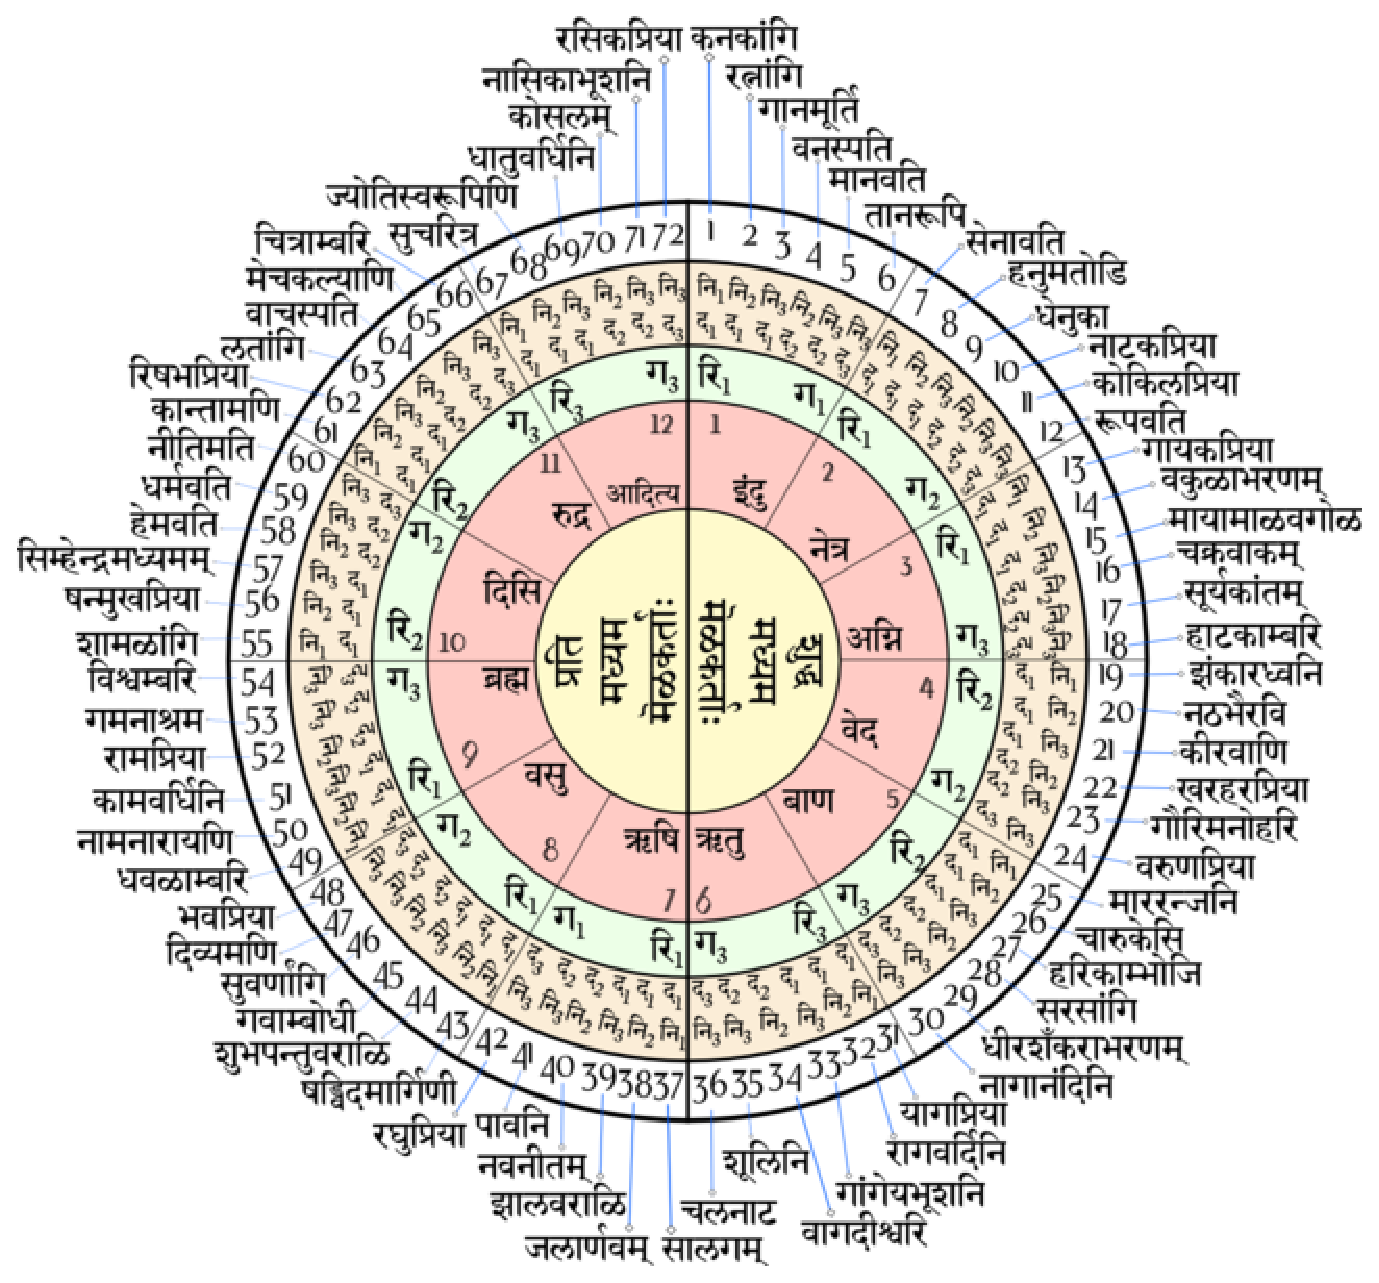
\includegraphics[scale=.4]{figures/7.eps}
\caption{Venkaṭamakhin’s\index{Venkatamakhin@Venkaṭamakhin} Mela-karta\index{Melakarta@\textsl{Mela-karta}} scheme}\label{chap3-fig5}
\end{figure}

Next we briefly discuss \textsl{tāla}\index{tala@\textsl{tāla}} which is widely known to have a mathematical content. In the distinctive style of percussion instruments such as \textsl{mṛdaṅga},\index{mrdanga@\textsl{mṛdaṅga}} we have \textsl{korapu} or \textsl{yati}-s\index{yati@\textsl{yati}} where phrases/duration have to be in arithmetic progression (increasing or decreasing). In addition, simple “diophantine” (another misnomer!) equations need to be solved to check feasibility of a \textsl{yati}. For example, there is the notion of \textsl{gati}\index{gati@\textsl{gati}}
 that fixes how many syllables can go into a time unit of \textsl{tāla}. This notion is independent of the specific \textsl{tāla} itself. While \textsl{caturaśra gati}\index{gati@\textsl{gati}}\index{gati@\textsl{gati}!caturasra@\textsl{caturaśra}} (4) is usually common, one can also attempt \textsl{triśra gati} (3), \textsl{khaṇḍa gati}\index{gati@\textsl{gati}!trisra@\textsl{triśra}}\index{gati@\textsl{gati}!khanda@\textsl{khaṇḍa}} (5), etc. Now if one is playing an iterative structure with a \textsl{yati}\index{yati@\textsl{yati}} also woven in but now with a \textsl{triśra} instead of \textsl{caturaśra}, the feasibility of this fitting into a given set of time units depends on solving some integer linear equation; if there is no solution, one has to creatively modify the structures by adding \textsl{virāma}-s or \hbox{\textsl{eḍupu}-s} (silent time units) to balance the equation but without destroying the aesthetic sense. Often, multiple solutions are possible, and they provide the variety seen. Some are quite tricky: for example, \textsl{sampūrṇa khaṇḍa naḍe} has 10 \textsl{akṣara}-s/8 units of \textsl{tāla}.

For a simpler example, consider 16 time units for a regular \textsl{tāla}\index{tala@\textsl{tāla}}\index{aditala@\textsl{āditāla}}\index{tala@\textsl{tāla}!adi@\textsl{ādi}} like \textsl{ādi tāla}. If \textsl{caturaśra gati}\index{gati@\textsl{gati}}\index{gati@\textsl{gati}!caturasra@\textsl{caturaśra}} is used, each \textsl{akṣara} could be $\sfrac{1}{4}$\,th of a time unit. If a \textsl{moharā} or \textsl{muktāyi} (both are reasonably complex pieces that are repeated 3 times to exactly match multiple complete durations of a cycle of \textsl{tāla} (“\textsl{āvartana}”)) is now attempted to be played in a different \textsl{gati} (say, \textsl{tiśra} where each \textsl{akṣara} is now $\sfrac{1}{3}$\,rd of a time unit), some \textsl{tālas} need adjustments; note that due to the “Vernier” principle, the time keeping has to be sufficiently exact otherwise, unresolved differences of $\sfrac{1}{3}-\sfrac{1}{4}$ time units ($\sfrac{1}{12}$\,th time unit) or its multiples will wreck the experience. In the most difficult case, $\sfrac{1}{7}- \sfrac{1}{9} = \sfrac{2}{63}$ time unit accuracy is needed!

There are many \textsl{tāla}-s (such as \textsl{Dhruva, Maṭhya, Jhampa, Aṭṭa, Eka}) and many variations with respect to time units and also \textsl{gati}.\index{gati@\textsl{gati}} It is difficult to remember the many sequences but experienced musicians remember high level patterns\index{patterns!rhythmic} but calculate some details on the fly! If they do not have sufficient time to calculate, then they play known simpler patterns till they can calculate the details right! A similar system obtains in the Hindustani\index{Hindustani music}\index{Indian Classical Music!Hindustani} (northern) system where for example \textsl{tabla}\index{tabla@\textsl{tabla}} is used; it is not uncommon to see somewhat unusual beats of 10 and half being played for half an hour! 

"\textsl{Pañcavādyam}"\index{Pancavadyam@\textsl{Pañcavādyam}}\index{temple art instrumental ensemble} a traditional temple art instrumental ensemble (\textsl{timila,\index{Pancavadyam@\textsl{Pañcavādyam}!timila@\textsl{timila}} maddalam,\index{Pancavadyam@\textsl{Pañcavādyam}!maddalam@\textsl{maddalam}} ilathalam}\index{Pancavadyam@\textsl{Pañcavādyam}!ilathalam@\textsl{ilathalam}} and \textsl{iḍakka}\index{Pancavadyam@\textsl{Pañcavādyam}!idakka@\textsl{iḍakka}} -- percussion; \textsl{kombu}\index{Pancavadyam@\textsl{Pañcavādyam}!kombu@\textsl{kombu}} -- wind instrument) of Kerala. The performance is led by the \textsl{timila} and the “sense of sacred” is generated by the pyramid-like rhythm structure with a constantly increasing tempo coupled with a proportional decrease in the number of beats in cycles.\\[-20pt]


\subsection{The Computational Basis of \textsl{Rasa} Architecture}\label{chap3-sec5.3}
\index{rasa@\textsl{rasa}}

\vskip -.1cm

Starting from the earliest times (5000 years and earlier?), the sense of the sacred was attempted to be given by geometry. The \textsl{śyena} geometry and its construction in the Vedic rites is a good example. Due to such examples and internal consistencies, A. Seidenberg argues for precedence of Vedic thought over Babylonians with respect to geometry (Seidenberg 1978).

Once the recursive structure of language (Pāṇini)\index{Panini@Pāṇini} and the number system have been mastered, it is an easy step to think of term rewriting rules (aXb$\to$pYq) or of mathematical series given by some (arithmetic/geo\-metric) progression. The Indic thinking (Hindu, Buddhist, Jaina), having gone past the stage of building perishable structures, started experimenting with stone to build long standing structures. For example, the superstructures of the \textsl{Nāgara} temples have a distinctive curvilinear form composed of a series of motifs with the surface geometry resulting from intricate mathematical and geometric expression based on stereotomic techniques (Kramrisch\index{Kramrisch, Stella} 1946:177), (Meister 1979).  A computational style thinking in such architectural ventures seems to have been common by 7-8 century C.E. already as we see in the majestic Ellora\endnote{“From The \textsl{Alas} inscription dated 770 C.E. tells us that the Kailasanath temple\index{Kailasanath temple} was commissioned in 757 C.E. (or 773 C.E.) by Kṛṣṇa I,\index{Krsna I@Kṛṣṇa I} an uncle of the founder of the Rāṣṭrakuta\index{Rastrakuta@Rāṣṭrakuta} dynasty, Dantidurga.\index{Dantidurga} The construction work took about 150 years to complete. ... While the entire temple complex looks like it is a cluster of temples and pillars and sprawling halls, it was actually carved out by \textsl{vertically} excavating some 200,000 tonnes (or 400,000 tonnes according to others) out of a \textsl{single}, mammoth rock. It cannot be emphasized enough that the real achievement is that the entire temple complex was \textsl{excavated, not constructed}. Indeed, it does evoke a sense of awe when we try and fathom what it must have taken in terms of mathematics, engineering, building technology, craftsmanship, artistry, design, planning, and the entire project execution when we recall that this “project” was executed over 150 years and spanned at least six generations of experts in all of these fields.” Indiafacts \url{http://www.indiafacts.co.in/ajanta-ellora-grandeur-cultural-amnesia-part-1} (Accessed on 27th July 2017)}; it seems to have reached its peak by 12 century C.E. (for example, Kandāriya temple in Khajuraho).\index{Khajuraho}

Trivedi discusses the use of recursive structures in Indic (especially Hindu/Jain) temples to depict an “evolving cosmos of growing complexity, which is self-replicating, self-generating, self-similar and dynamic” (Trivedi 1989:249). Furthermore, “the procedures are recursive and generate visually complex shapes from simple initial shapes through successive application of production rules that are similar to rules for generating fractals.”\index{fractals} The techniques identified are 
\begin{itemize}
\item[(i)] \textbf{Fractalization}. A very simple example is going from n sides for a pillar to 2n sides next and repeat till we approach the shape of a circle; this can be seen in many temples where pillars with 4, 8, 16 sides and circles can be seen in the same enclosure. Similarly, Koch-like fractals\index{fractals}\index{fractals!Koch fractals} are generated but on initial shapes more complex than a simple line. For example, for Koch fractal, the shape -------- is first transformed to ----/$\backslash$---- and each small segment is similarly transformed; if this procedure is repeated, the resulting shape is similar to the plans of some Hindu temples that display the “snowflake curves characteristic of fractal figures” (see figures 2 and 3 in (Trivedi 1989)). The architectural texts discuss these techniques explicitly and also develop a vocabulary to describe the process (see figure 17 in (Trivedi 1989)). The self-iteration can be \textsl{dvi-aṅga} (adding 2 more segments \textsl{karṇa} and \textsl{bhadra} where 1 existed), \textsl{tri-aṅga} (adding one more segment \textsl{pratiratha} to the \textsl{dvi-aṅga}), \textsl{caturaṅga} (adding segment \textsl{nandikā} to \textsl{tri-aṅga}), \textsl{pañcāṅga} (adding \textsl{koṇikā}), etc. 

\item[(ii)] \textbf{Self-similar Iteration in a Decreasing Scale}. Rules such as \textsl{triguṇa sūtra} and \textsl{ṣaḍguṇa sūtra} are given in \textsl{Samarāṅgaṇasūtradhara} that give the method of iteration (Kramrisch 1926:209).  Discussing the geometry of temples, Sambit Datta says “The surface of the superstructure is composed of a series of carved motifs that exhibit a progressively diminishing sequence of self-similar forms. While no guide exists in the canonical literature on how these sequences are handled, two clues are available in the mathematical and cosmological texts. First, the notion of \textsl{shunyata} [\textsl{śūnyatā}] (nothingness) and the infinitesimally small occupies a central place in the syncretic Upanishadic cosmology. Second, the preoccupation with and knowledge of \textsl{shredhikshetras} [\textsl{śreḍhī-kṣetra}-s] (mathematical series) are evident in Vedic mathematical texts.” (Dutta 2010:479). Furthermore, Datta (2010:477) “developed a mathematical procedure to generate the curvature based on textual descriptions. This procedure is dependent on the height of the superstructure, the number of vertical units chosen for each offset and the choice of an integer (one of 3,4,5,7) for controlling the degree of curvature.” Assuming a reduction by $\sfrac{1}{4}$\,th to control the curvature, the geometric series is given by $\sfrac{\text{H}}{4}$, $\sfrac{3}{4}$.$\sfrac{\text{H}}{4}$, $\sfrac{3}{4}$.$\sfrac{3}{4}$.$\sfrac{\text{H}}{4}$, ... where H is the height of superstructure.

\item[(iii)] \textbf{Repetition, Superimposition, and Juxtaposition.}
\end{itemize}

Note that working with series of pillars with 4, 8, 16, ... sides as it approaches a circle or the more complex fractal\index{fractals} series in temple architecture may have provided the practical examples and also the intuition to Indian mathematicians on how to understand infinite sequences, with brilliant results such as Mādhava’s series\index{Madhava series@Mādhava series for Pi}\index{Gregory series@``Gregory” series} for pi (misnamed later as “Gregory” series) in the 13th century C.E., faster convergent series for pi in the Kerala school of mathematics from the 14 century C.E., etc.

Temples also incorporate astronomical aspects (for example at Konārak);\index{Konarak} this requires architectural planning with mathematical precision. Boner says 

\begin{myquote}
...the temple must, in its space-directions, be established in relation to the motion of the heavenly bodies. But in as much as it incorporates in a single synthesis the unequal courses of the Sun, the Moon and the planets, it also symbolizes all recurrent time sequences: the day, the month, the year and the wider cycles marked by the recurrence of a complete cycle of eclipses, when the sun and the moon are readjusted in their original positions, a new cycle of creation begins. 

\hfill(Boner 1966:XXXIII)
\end{myquote}

An excellent example of this deep and all-encompassing vision can be seen in Angkor Wat where the dimensions reflect the \textsl{yuga} durations, the entrances correspond to the positions of the Sun, the Moon and the planets during equinoxes, etc. (Stencel \textsl{et al} 1976) In a sense, a temple is a mathematically constrained object carefully engineered with multiple objectives: human, divine and celestial. To effect astronomical recurrences in a temple, a computational iterative basis can only be surmised as only kinematic aspects were known. It is interesting also to note that such considerations are present in the mathematical realization of \textsl{maṇḍala}-s\index{mandala@\textsl{maṇḍala}} used in worship; Huet discusses the mathematical complexity of a \textsl{Śrīcakra}\index{Sricakra@\textsl{Śrīcakra}} (Huet 2002). While a constraint system has been developed to model the Śrīcakra, similar models may have been inspired by the practical abstractions needed by a temple architect, especially to work out the recurrent astronomical time sequences.\\[-20pt]

\subsection{The Computational Basis of \textsl{Rasa} in Varied “Crafts”}\label{chap3-sec5.4}
\index{rasa@\textsl{rasa}}

Aesthetic designed repeated structures (sometimes with subtle changes) are seen widely in Indic crafts such as \textsl{rangoli}\index{rangoli@\textsl{rangoli}} (“space-filling curves”), cloth-making as well as in civil works such as wells. A \textsl{rangoli} is given below (figure \ref{chap3-fig6}) drawn recently by a person who has most likely never heard of fractals,\index{fractals} yet it resembles them in a significant way. Due to space constraints\endnote{For details see Yanagisawa\index{Yanagisawa, Kiwamu} (2007), Waring\index{Waring, Timothy} (2012).}, we do not discuss these further except to point out the innovations in the engineering of the musical “\textsl{rasa}”\index{rasa@\textsl{rasa}} in \textsl{mṛdaṅga,\index{mrdanga@\textsl{mṛdaṅga}} vīṇā} etc.

The construction of instruments such as \textsl{mṛdaṅga, vīṇā} and \textsl{tambūra}\index{vina@\textsl{vīṇā}}\index{tambura@\textsl{tambūra}} in the past has showed an amazing intuitive feel for effecting aesthetically unusual features not found in other instruments elsewhere. Only in the last few decades, by experimental/computational modelling, has this been understood. For example, \textsl{mṛdaṅga} and \textsl{tabla}\index{tabla@\textsl{tabla}} are unusual and different from almost any other types of drums in other parts of the world: it has a harmonic character which only stretched/\-stringed instruments usually have. The composite nature of the skins as well as “\textsl{karaṇi}” (circular black part made of a metallic paste) play an important part.  CV Raman\index{Raman, C. V.} and Kumar discovered only 4 significant overtones (Raman 1920); for example, f, 2f, 3f, 4f and 5f tones are present but other harmonics and all non-harmonics suppressed to a great extent. Other drums or stretched membranes elsewhere (including \textsl{kañjīra}!) sound harsh as they abound in non-harmonics. Interestingly, there is similar surprise with \textsl{vīṇā/sitār/tambūra}\index{vina@\textsl{vīṇā}}\index{tambura@\textsl{tambūra}}\index{sitar@\textsl{sitār}} where the strings/curved bridge design along with a cotton thread between them for finer control is used to get overtone rich sounds (Raman 1921). It is not clear how our ancestors/artisans intuited them; even more surprising is the black patch on the \textsl{baayan} (left side) of the \textsl{tabla} pair; it is off-center! B S Ramakrishna discusses them in detail along with experiments to explain the unusual harmonic nature of \textsl{mṛdaṅga}\index{mrdanga@\textsl{mṛdaṅga}} and \textsl{tabla}\index{tabla@\textsl{tabla}} (including the off-center patch of the \textsl{baayan}) (Ramakrishna 1994). Furthermore, Gauthier, Leger \textsl{et al.} remark 

\begin{myquote}
“Raman also concluded that the first nine modes of vibration having the lowest frequencies give a harmonic sequence of only five tones which means that some of these modes are degenerate, i.e. have approximately the same frequency. It is worth recalling that the theory of ordinary drumheads does not predict even approximate degeneracies of any of the modes or any harmonic relationships between them.” 

... [T]he following questions related to the evolution of the table and mṛdanga arise: How did Indian artisans and musicians discover, more than 2000 years ago, an optimal configuration for these drums among an infinite number of possible configurations?” 
\hfill (Gaudet 2006:389)
\end{myquote}
\begin{figure}[H]
\centering
\includegraphics[scale=.65]{figures/8.eps}
\caption{Rangoli\index{rangoli@\textsl{rangoli}} pattern drawn by an artist}\label{chap3-fig6}
\end{figure}

\section{Conclusions}\label{chap3-sec6}

In the above discussion, we hope to have convinced the reader that Pollock\index{Pollock, Sheldon} may have been off the mark when he made a categorical statement that Indian thinkers did not try to understand the well-springs of \textsl{pratibhā}.\index{pratibha@\textsl{pratibhā}} We argue that this may be located in a computational model for \textsl{rasa};\index{rasa@\textsl{rasa}} existing implicitly perhaps but all the same noticeable if seen with the right perspective. We have only sketched an outline here. Similarly, the charge of lack of anything common across the \textsl{kalā}-s\index{kala@\textsl{kalā}} may also seen to be blunted by our showing that a computational thinking across these domains also permeated their endeavours.

{\appendix
\section{APPENDIX}\label{chap3-app1}

\rhead[]{3. Towards a Computational Theory for {\sl Rasa:}\quad\small\thepage}

\subsection*{Brief background on Computational Thinking}

Two fundamental aspects of computer science, as Bhate\index{Bhate, Saroja} and Kak\index{Kak, Subhash} put it, are the creation of new computing algorithms and machines that have powerful computational and cognitive abilities (Bhate 1993): this includes development of new techniques of representing and manipulating knowledge, inference and deduction. Also, in a long term perspective, it is the development of techniques that make the elucidation of the computational structure of nature and the mind easier.

Consider an extremely simple but early attempt at quantifying levels of happiness in \textsl{Taittirīya Upaniṣad} (2.7.1-4) where it gives 10 levels of “\textsl{ānanda}" starting from one, and increasing in geometric progression (1 to \verb|10^20|) in steps of 100x\endnote{Note curiously that the limit of happiness saturating or overflowing at \verb|10^20| (\textsl{Brahmā\-nanda}) is just beyond the native integer capability of current 64-bit machines\break (\verb|10^18<2^64<10^20|)!}. While such gradations are difficult to describe or may be even defend, it gives an idea of the enormousness of the \textsl{sādhanā} needed to reach \textsl{Brahman}, as 1 is said to be the happiness of a healthy youth in the prime of life. One can even argue that such quantification early on helped in understanding the iterative/recursive nature of the number system with time.

As another simple example, consider Suśruta:\index{Susruta@Suśruta} he is interested in how many ways one can combine different tastes ("\textsl{ruci}") and in the process enumerates one of the earliest known example of combinatorics\index{combinatorics} in \textsl{Caraka Saṁhitā},\index{Caraka Samhita@\textsl{Caraka-saṁhitā}} a text that is atleast 2000+ years old. The specific question: if medicine can be sweet, sour, salty, peppery, bitter or astringent, how many possibilities are there 

if we mix any 2 qualities? It is listed as 15 possibilities ($^{6}$C$_{2}$).\\[2pt]
Similarly, if we mix any 3 qualities? 20 possibilities ($^{6}$C$_{3}$);\\[2pt]
any 4 qualities? 15 possibilities ($^{6}$C$_{4}$);\\[2pt]
any 5 qualities? 6 possibilities ($^{6}$C$_{5}$) and\\[2pt]
any 6 qualities? only 1 possibility ($^{6}$C$_{6}$).


Taking next a well known example, the recursive structure of the number system was first grasped by the Indic civilization in all its fullness (as well by only one other, the Mayan, as per recent understanding) and it then spread to others. In a sense, the journey towards computational thinking had begun; we will discuss what this means briefly below. The other most successful recursive example is that of Pāṇini’s\index{Panini@Pāṇini} innovative generative grammar for Vedic and later Sanskrit, which has been described as the “one of the greatest monuments of human intelligence” (Bloomfield 1933:11). We do not discuss this further as it has been discussed extensively.

For a visual and more easily accessible example, consider the Kandāriyā Mahādeva temple (part of Khajuraho\index{Khajuraho} temple) that is best explainable as constructed on the basis of a set of recursive rules. Visually, the structure is striking but at the root of it is a set of recursive rules, as (Trivedi 1989) and (Dutta 2010) show.

If we look at computational thinking in early India, we see very good examples with respect to:
\begin{itemize}
\itemsep=2pt
\item[(i)] Grammarians e.g., Pāṇini,\index{Panini@Pāṇini} Kātyāyana, Patañjali (Grammar $\sim$ computation, now established in computer science).

\item[(ii)] Logicians e.g., Gautama, Udayana, Gaṅgeśa, Raghunātha Śiromaṇi\index{Katyayana@Kātyāyana}\index{Patanjali@Patañjali}\index{Gautama}\index{Udayana}\index{Gangesa@Gaṅgeśa}\index{Raghunatha Siromani@Raghunātha Śiromaṇi} (Logic $\sim$ computation, also now established in computer science).

\item[(iii)] Connections with “cognitive science” or “inner sciences” like Yoga with respect to mind sciences (psychology, neuroscience). This is becoming very pronounced in the last decade in computer science and related fields.
\end{itemize}

In an influential paper, viz.~Wing (2006:33), the two A’s of “Computational Thinking” are given as 

\newpage

\begin{itemize}
\itemsep=2pt
\item[(i)] Abstraction which operates in terms of multiple layers of abstraction simultaneously and that defines the relationships the between the layers

\item[(ii)] Automation which mechanizes abstraction layers and their relationships
\end{itemize}


Mechanization is possible due to precise and exacting notations and models; note that the Indic number system was the 1st non-trivial example which had this property. Also, this “machine” can be human or computer, virtual or physical. For example, Pāṇini’s\index{Panini@Pāṇini} generative grammar was sufficiently internalized for the Sanskrit language that any literate person had to know it well to use/debate with these rules to decide on the correctness of some intricate question of semantics or word-formation.

Computational Thinking more broadly can be seen as Abstraction, Mechanization, Recursion and Bootstrapping; these give us the ability and audacity to scale. Interestingly, many of these were being handled in our tradition, but in this paper, we mostly discuss those connected with \textsl{rasa}.\index{rasa@\textsl{rasa}}

\section{APPENDIX}\label{chap3-app2}

\vskip .1cm

\subsection*{Brief Background on Computational Thinking in Indic Tradition}

\vskip .1cm

Let us briefly look at why a computational approach for \textsl{rasa} may be useful by looking at a different area, that for mathematics or astronomy. There is a need for a healthy dose of empiricism in complex domains of enquiry; this enabled, for example, the early Indian mathematicians to work on approximations (infinite series) that the Western (“European”) mathematics could not comprehend or become comfortable with except past 17th century. Roddam Narasimha\index{Narasimha, Roddam} discusses "computational positivism"\index{Computational Positivism} as a distinguishing property of Indian approach to mathematics (Narasimha 2003); it was based not on, for example, some indefensible metaphysics, for example, of the Greeks (e.g., “circles are perfect shapes, all planets need to be explained as moving in circles, hence epicycles”) but on diverse models that each needed to evaluated for suitability (\textsl{Siddhānta Śiromaṇi}\index{Siddhanta Siromani@\textsl{Siddhānta Śiromaṇi}} of Bhāskara\index{Bhaskara@Bhāskara}\index{Siddhanta Siromani@\textsl{Siddhānta Śiromaṇi}} II: dṛg-gaṇitaikya). 

We summarize some of his deep insights here. The basic position historically has mostly either been a deductive/ “logical” one of the Greeks, or the “Computational Positivism”\index{Computational Positivism} of the Indics (note that other cultures may have some component of either but we will take Greek and Indic as exemplars). The latter attitude, often implicitly and occasionally explicitly, informed the classical Indian mathematical approach to astronomy. \textsl{Āryabhaṭīya},\index{Aryabhatiya@\textsl{Āryabhaṭīya}} for example, “provides short, effective, methods of calculation rather than a basic model from which everything can be deduced”; essentially, it describes algorithmic or computational astronomy. This is opposite of Euclidean method of going from well stated axioms through a process of purely logical deduction to theorems or conclusions. After \textsl{Āryabhaṭīya},\index{Aryabhatiya@\textsl{Āryabhaṭīya}} a profusion of diverse ideas in mathematics then ensued such as the development and flowering of trigonometry in India and innovative solving of intricate integer quadratic equations such as \textsl{Cakravāla} in an algorithmic way; these finally found their way to Europe through Persia and Arabia.

Positivism\index{Computational Positivism} posits that facts are the only possible objects of knowledge and science the only valid knowledge; there is no need for metaphysics! 'Logical' positivism of the famous Vienna Circle (scientists, mathematicians and philosophers) in first half of 20th~c. had the central tenet of verifiability: “a statement that cannot be verified is held to be automatically meaningless”. There are in this perspective only two types of meaningful statements: the necessary truths of logic, mathematics and language, and empirical propositions about the rest of the world, with Wittgenstein positing that propositions of logic and mathematics are tautologies! However, Godel and Popper in the 1930’s demolished this school of thought comprehensively in their own ways. 

Computational Positivism,\index{Computational Positivism} as argued by Roddam Narasimha\index{Narasimha, Roddam} (2003), is that computation and observation, when in agreement, constitute the only form of valid knowledge; models, logic, metaphysics etc. are either secondary or not relevant. Models may not be unique (in the sense that different models may yield very similar results in a domain of interest).

\newpage

The best example in India is that of the Kerala school of mathematics, a group of astronomers and mathematicians who, over a period of some three centuries, produced some very innovative and powerful mathematics applied to astronomy. The basic goal is that of \textsl{dṛg-gaṇitaikya}, the identity of the seen and the computed. There is an effort to find “best” algorithms or computational procedures that made the best predictions as determined by comparison with observation as, over a period of time, discrepancies between computation and observation tend to increase. Nīlakaṇṭha\index{Nilakantha@Nīlakaṇṭha} (1444-1545 C.E.) explicitly says “the best mathematicians have to sit together and decide how the algorithms have to be modified or revised to bring computation back into agreement with observations!”. Hence this approach is closer to experimental mathematics and also close to how modern science views models and observations. Surprisingly, Kepler\index{Kepler, Johannes} in his \textsl{Astronomia Nova}\index{Astronomia Nova@\textsl{Astronomia Nova}} (1609 C.E.) displays a similar computational perspective in his analysis of the motion of Mars, so different from the largely ineffectual “axiomatic” thinking, dominant at that time, for that specific problem.

One way to understand what was happening in the Indic sphere with respect to \textsl{rasa}\index{rasa@\textsl{rasa}} in the past is similar to what has been happening in the study of hard sciences post 1500 C.E. where mathematics has become central; note that now fields such as computational linguistics, computational neuroscience, etc. as well as computer-based music or architecture are flourishing. The Indic world had understood the recursive nature of number system and that of language by the 1st few centuries C.E. and hence such recursive structures gave an impetus to computational thinking in diverse fields. Other civilizations around that time had not sensed it by that time and only the transmission of Indic ideas into Arabia by 8th century C.E. and by 12th century C.E. into Europe put them on to such thinking. 

Tragically, just as the Indic world was flowering with such ideas, its autonomy was lost with the annihilation of its intellectual class in Kāśmīra and other areas in North India coupled with a sense of the siege in the South, and the stream of innovative ideas based on such conceptions were mostly extinguished by the 16th-17th century C.E..
}

\begin{thebibliography}{99}
\itemsep=2pt
\bibitem[]{chap3_item1}
Apte, V.S. (1957-59). \textsl{The Practical Sanskrit-English Dictionary}.  Accessed at (\url{http://dsal.uchicago.edu/dictionaries/apte/})

\bibitem[]{chap3_item2}
Bary, Theodore de, Hay, S., Weiler, R., Yarrow, A. (Ed.s) (1963). \textsl{Sources of Indian Tradition}. New Delhi: Motilal Banarsidass.

\bibitem[]{chap3_item3}
Beitmen, Logan R. (2014). ``Neuroscience and Hindu Aesthetics: A Critical Analysis of V.S. Ramachandran's ``Science of Art''''. \textsl{Florida International University (FIU) Electronic theses and Dissertations.} Paper no:1198.

\bibitem[]{chap3_item4}
{\sl\bfseries Bharatārṇava} of Nandikeśvara. See Gairola (2013).

\bibitem[]{chap3_item5}
Bhate, Saroja and Kak, Subhash. (1993). “Pāṇini’s Grammar and Computer Science”. \textsl{Annals of Bhandarkar Oriental Research Institute}, 72. pp.~79--94.

\bibitem[]{chap3_item6}
Bloomfield, Leonard. (1933). \textsl{Language}. New York: Henry Holt.

\bibitem[]{chap3_item7}
Boner, Alice. and Śarmā, Sadāśiva Rath. (1966). \textsl{Śilpa Prakāśa Medieval Orissan Sanskrit Text on Temple Architecture}. Leiden: EJ Brill.

\bibitem[]{chap3_item8}
Bronner, Yigal. (2010). \textsl{Extreme Poetry}. Columbia: Columbia University Press.

\bibitem[]{chap3_item9}
Chakrabarti, Arindam. (Ed.) (2016). \textsl{The Bloomsbury Research Handbook of Indian Aesthetics and the Philosophy of Art}. Manoa, USA: Bloomsbury Academic.

\bibitem[]{chap3_item10}
Cole, J (Ed.) (1972). \textsl{Nebraska Symposium on Motivation}. Lincoln, NB: University of Nebraska Press.

\bibitem[]{chap3_item11}
Coward, Harold G. and Raja, Kunjunni. (1990). “Metaphysics: Shabda Brāhman and its manifestations”. In Potter (1990). pp.~33--38.

\bibitem[]{chap3_item12}
Dalgleish, T. and Power, M. (Ed.s) (1999). \textsl{Handbook of Cognition and Emotion}. Sussex, UK: John Wiley \& Sons Ltd.

\bibitem[]{chap3_item13}
Dennett, Daniel. (1988) "Quining Qualia." In Marcel and Bisiach (1988). pp.~42--77.

\bibitem[]{chap3_item14}
---\kern3pt(1992). \textsl{Consciousness Explained}. USA:Back Bay Books.

\bibitem[]{chap3_item15}
di Pellegrino, G., Fadiga, L., Foggassi, L., Gallese, V., and Rizzolatti, G. (1992) “Understanding motor events: a neurophysiological study,” \textsl{Experimental Brain Research.} 1992; 91(1). pp.~176--180.

\bibitem[]{chap3_item16}
Dutta, Sambit. (2010) “Infinite Sequences in the Constructive Geometry Of Tenth-Century Hindu Temple  Superstructures”. \textsl{Nexus Network Journal} 12 (2010). pp.~471--483.

\bibitem[]{chap3_item17}
Ekman, Paul. (1999). ``Universals and Cultural Differences in Facial Expressions of Emotions.'' In Cole, J. (1972). pp.~207--282.

\bibitem[]{chap3_item18}
---\kern3pt(1972). ``Basic Emotions''. In Dalgleish and Power (1999). pp.~45--60.



\bibitem[]{chap3_item19}
Gairola, Vachaspati. (Ed.) (Trans.) (2013). \textsl{Bharatārṇavaḥ of Nandikeśvara}. Vol.~242. Varanasi: Chowkhamba Krishnadas Academy.

\bibitem[]{chap3_item20}
Gala, Nuria., Rapp, Reinhard., Bel-Enguix, Gemma (Ed.s) (2015) \textsl{Language Production, Cognition, and the Lexicon}. Basel:Springer International Publishing.

\bibitem[]{chap3_item21}
Gambhirananda, Swami. (2000) \textsl{Eight Upanishads}. Calcutta: Ramakrishna Mission.

\bibitem[]{chap3_item22}
Gaudet, Samuel. Gauthier, Claude. and Legér, Sophie. (2006). “The evolution of harmonic Indian musical drums: A mathematical perspective”. \textsl{Journal of Sound and Vibration} 291. pp.~388--394.

\bibitem[]{chap3_item23}
\textsl{Gīta Govinda}. See Narayanan and Mohan (2016).

\bibitem[]{chap3_item24}
Ghosh, Manmohan. (1957). \textsl{Nandikeshwara’s Abhinayadarpana}. Calcutta: Firma Mukhopadhyaya.

\bibitem[]{chap3_item25}
Gratch, Jonathan and Marsella, Stacy. (2009). "Modeling the cognitive antecedents and consequences of emotion”. \textsl{Journal of Cognitive Systems Research}, Vol.~10, no.~1. pp.~1--5.

\bibitem[]{chap3_item26}
Hameroff . Stuart., and Penrose, Roger. (2014). “Consciousness in the universe: A review of the ‘Orch OR’ theory”. \textsl{Physics of Life Reviews}, Volume 11, Issue 1, March 2014. pp.~39--78.

\bibitem[]{chap3_item27}
Herzberger, Hans and Herzberger, Radhika. (1981) Bhartṛhari's Paradox”. \textsl{Journal of Indian Philosophy}. 9. pp.~1--17.

\bibitem[]{chap3_item28}
Hofstadter, Douglas. (1979). \textsl{Escher, Godel, Bach}. New York:Basic Books.

\bibitem[]{chap3_item29}
Hogan, Patrick. (1996) \textsl{College Literature} 23.1 (February 1996). pp.~164--178.

\bibitem[]{chap3_item30}
---\kern3pt(2003a). “\textsl{Rasa} Theory and Dharma Theory”. \textsl{Quarterly Review of Film and Video}. 20. pp.~37--52.

\bibitem[]{chap3_item31}
---\kern3pt(2003b). \textsl{The Mind and Its Stories}. Cambridge: Cambridge University Press.

\bibitem[]{chap3_item32}
Hoskote, Ranjit. (2011). \textsl{I, Lalla: The Poems of Lal Ded}. New Delhi: Penguin Books.

\bibitem[]{chap3_item33}
Houben, Jan. (1995). “Bhartṛhari's solution to the liar and some other paradoxes”. \textsl{Journal of Indian Philosophy} 23. pp.~381--401.

\bibitem[]{chap3_item34}
Hovy, Eduard (2015) “What are Sentiment, Affect and Emotion? Applying the Methodology of Michael Zock to Sentiment Analysis”. Gala \textsl{et al} (2015). pp.~13--24.

\bibitem[]{chap3_item35}
Huet, G. (2002). “Sri Yantra Geometry”. \textsl{Theoretical Computer Science} 281 (2002). pp.~609--628.

\bibitem[]{chap3_item36}
Iyengar, R.N. (2017) “Concept of Probability in Sanskrit Texts on Classical Music” ICPR conf (“S\&T in the Indic Tradition”, Feb 2017, IISc) video proceedings: \url{https://livestream.com/shaalelive/iisc}. Accessed on 3rd January 2018.

\bibitem[]{chap3_item37}
Jain, Anupam., Rakhi, N. K., and Bagler, Ganesh. (2015). \textsl{Spices form the basis of food pairing in Indian cuisine}. \url{https://arxiv.org/pdf/1502.03815}. Accessed on 3rd January 2018.

\bibitem[]{chap3_item38}
Janata, Petr. (2014). “In Search of neural correlates of spiritual experiences with music,” \url{https://ccrma.stanford.edu/events/matb/program.html}, Stanford University. Accessed on 3rd January 2018.

\bibitem[]{chap3_item39}
Joshi, Aditya., Bhattacharyya, Pushpak. and Carman, Mark J. (2018) “Automatic Sarcasm Detection: A Survey”. \textsl{ACM Computing Surveys}. Article No.~1000.

\bibitem[]{chap3_item40}
Jourdain, Robert. (2008). \textsl{Music, the Brain, and Ecstasy: How Music Captures Our Imagination}. New York:William Morrow.

\bibitem[]{chap3_item41}
Kak, Subhash. (2004). “The Golden Mean and the Physics of Aesthetics,” Archive of Physics: physics/0411195.

\bibitem[]{chap3_item42}
---\kern3pt(2005). “Recursionism and Reality: Representing and Understanding the World” Baton Rouge:Lousiana State University.

\bibitem[]{chap3_item43}
---\kern3pt(2008). \textsl{Mind and Self}. Stillwater: Oklahoma State University.

\bibitem[]{chap3_item44}
Kannan, K.S. (Ed.) (2018). \textsl{Western Indology on Rasa -- A Pūrvapakṣa}. Chennai: Infinity Foundation India.

\bibitem[]{chap3_item45}
Kapoor, Kapil. (2000). “Eleven Objections to Sanskrit Literary Theory: A Rejoinder”. Infinity Foundation, \url{http://www.infinityfoundation.com/mandala/s_es/st_es_kapoo_eleven_frameset.htm}. Accessed on 25th January 2017.

\bibitem[]{chap3_item46}
---\kern3pt and Danino, Michel. (Ed.s) (2012). \textsl{Knowledge Traditions and Practices of India}. New Delhi: CBSE.

\bibitem[]{chap3_item47}
Kashyap, R. L. and Bell, M. R. (1998). \textsl{Error Correcting Code-like Chanting Procedures in Ancient India}. Bangalore: Sri Aurobindo Kapali Shastry Institute of Vedic Culture, Sakshi.

\bibitem[]{chap3_item48}
Kaviraj, Gopinath. (1966). “Doctrine of Pratibhā in Indian Thought”. \textsl{Annals of Bhandarkar Oriental Research Institute}, Pune 1923-24.

\bibitem[]{chap3_item49}
Knuth, D. E. (1990) \textsl{The Genesis of Attribute Grammars}. WAGA Proceedings of the International Conference on Attribute Grammars and Their Applications. pp.~1--12. Paris, France.


\bibitem[]{chap3_item50}
---\kern3pt(1997). \textsl{Art of Computer Programming}. Reading, MA: Addison Wesley.

\bibitem[]{chap3_item51}
---\kern3pt(2011). \textsl{Art of Programming}. Vol.~IV A. Upper Saddle River, NJ: Addison Wesley.

\bibitem[]{chap3_item52}
Kramrisch, Stella. (1928). \textsl{The Vishnudharmottara. Part III. A Treatise on Indian Painting and Image-making}. Calcutta: Calcutta University Press.

\bibitem[]{chap3_item53}
---\kern3pt(1976, 1946$^{1}$). \textsl{The Hindu Temple}. Vol I. Calcutta: University Of Calcutta.

\bibitem[]{chap3_item54}
Lath, Mukund. (1984). “Bharata and the fine art of Mixing Structures”. Workshop on “System” “Structure” and “discourse”. (March 1984). Department of Sociology, University of Delhi. \url{http://www.svabhinava.org/abhinava/MukundLath/Bharata-frame.php}. Accessed on 3rd January 2018.

\bibitem[]{chap3_item55}
---\kern3pt(2016). “Thoughts on \textsl{Svara} and \textsl{Rasa}: Music as Thinking and Thinking as Music”. In Chakrabarti (2016). pp.~93--106.

\bibitem[]{chap3_item56}
Loorits, Kristjan. (2014). “Structural qualia: a solution to the hard problem of consciousness”. \textsl{Frontier Psychology}, 18 March 2014.

\bibitem[]{chap3_item57}
Malhotra, Rajiv. (2014). \textsl{Indra’s Net}. Noida: Harpercollins Publications.

\bibitem[]{chap3_item58}
---\kern3pt(2016). \textsl{The Battle for Sanskrit}. Noida: Harpercollins Publications.

\bibitem[]{chap3_item59}
Marcel, A. and Bisiach, E. (Ed.s) (1988) \textsl{Consciousness in Modern Science}. Oxford: Oxford University Press.

\bibitem[]{chap3_item60}
Marsella, Stacy., Gratch, Jonathan., and Petta, Paulo. (2010) “Computational Models of Emotion”. \textsl{Blueprint for Affective Computing (Series in Affective Science)}, no.~2010. London:Oxford University Press.

\bibitem[]{chap3_item61}
Meister, M. W. (1979) “Mandala and Practice in Nagara Architecture in N.India.”. \textsl{Journal of American Oriental Society}. 99. pp.~204--219.

\bibitem[]{chap3_item62}
Menon, Sangeetha. (2011) “A First Person Approach to Aesthetic Emotions in NātyaShāstra”. In Narasimha and Menon (2011). pp.~259--270.

\bibitem[]{chap3_item63}
Mukherjee, Sujit. (1981). \textsl{Some Positions on a Literary History for India.} Mysore: Central Institute for Indian Languages.

\bibitem[]{chap3_item64}
Nagraj, P. (1989). “Mārga and Desi in narrative”, National Seminar on Narratology of Indian Literature, Telugu University.

\bibitem[]{chap3_item65}
---\kern3pt(2016). Personal Communication.

\bibitem[]{chap3_item66}
Narasimha, Roddam. (2003). “Axiomatism and computational positivism,” \textsl{Economic and Political Weekly}. Vol. 38, No.~35. pp.~3650--3656.

\bibitem[]{chap3_item67}
Narasimha, Roddam., and Menon, Sangeetha. (Ed.s) (2011) \textsl{History of Science, Philosophy and Culture in Indian Civilization}, Vol XIV, Part 1, Nature and Culture. New Delhi: Munshiram Manoharlal.

\bibitem[]{chap3_item68}
Narayanan, Sharda and Mohan, Sujatha. (2016) \textsl{Gīta Govinda}. Chennai: Ambika Aksharavalli.

\bibitem[]{chap3_item69}
Narayanan, Vasudha. (2002) “Embodied Cosmologies: Sights of Piety, Sites of Power”. \textsl{Journal of the American Academy of Religion}, September 2003, Vol.~71, No.~3. pp.~495--520.

\bibitem[]{chap3_item70}
{\sl\bfseries Nāṭyaśāstra} of Bharata. See Rastogi (2016).

\bibitem[]{chap3_item71}
Oizumi, M. Albantakis, L., and Tononi, G. (2014). ``From the Phenomenology to the Mechanisms of Consciousness: Integrated Information Theory 3.0." \textsl{PLoS Computational Biology} 10(5): e1003588. doi:10.1371/journal.pcbi.1003588. 

\bibitem[]{chap3_item72}
Orpwood, Roger. (2013). “Qualia could arise from information processing in local cortical networks”. \textsl{Frontier Psychology}, 2013;4:121. doi:10.3389/fpsyg.2013.00121.

\bibitem[]{chap3_item73}
Pillai, Raghavan, K. (1971) \textsl{The Vākyapadīya}. New Delhi: Motilal Banarsidass.

\bibitem[]{chap3_item74}
Pollock, Sheldon (2016) \textsl{The Rasa Reader}. New York: Columbia University Press.

\bibitem[]{chap3_item75}
Potter, Karl. (1990). \textsl{Philosophy of the Grammarians.} Volume 5 of \textsl{Encyclopedia of Indian Philosophies}. New Delhi: Motilal Banarsidass.

\bibitem[]{chap3_item76}
Raghavan, V. (1963). “Kama: the Third End of Man”. In de Bary et al (1963). pp.~258--275.

\bibitem[]{chap3_item77}
Ramachandran, V. S., and Hirstein, William (1999) “The Science of Art: A Neurological Theory of Aesthetic Experience”. \textsl{Journal of Consciousness Studies}. pp.~15--51.

\bibitem[]{chap3_item78}
Ramakrishna, B. S. (1994). “Physics of Indian Drums”. Talavadya Seminar 1, Karnataka Sangeetha Nrithya Academy, Baṅgalore.

\bibitem[]{chap3_item79}
Raman, C. V. and Kumar, Sivakali. (1920). “Musical Drums with Harmonic Overtones”. \textsl{Nature} Vol.~104. p.~500.

\bibitem[]{chap3_item80}
---\kern3pt(1921). “On Some Indian Stringed Instruments”. \textsl{Proceedings of Indian Association for the Cultivation of Science 7}. pp.~29--33.

\bibitem[]{chap3_item81}
Rao, Sreenivasa (2008). “The Art of Painting in Ancient India -- Citrasutra” (\url{http://creative.sulekha.com/the-art-of-painting-in-ancient-india-Citrasutra-2_364304_blog}). Accessed on 3rd January 2018.

\bibitem[]{chap3_item82}
---\kern3pt(2012). "The Art of Painting in Ancient India -- Chitrasutra (6)". (\url{https://sreenivasaraos.com/tag/vishnudharmottara/}). Accessed on 3rd January 2018.

\bibitem[]{chap3_item83}
---\kern3pt(2017). \url{https://sreenivasaraos.com/tag/dhvani/}. Accessed on 3rd January 2018.

\bibitem[]{chap3_item84}
Rao, Velcheru Narayana., Shulman, David (2012). \textsl{Śrīnātha : the Poet who Made Gods and Kings}. New York: Oxford University Press.

\bibitem[]{chap3_item85}
Rastogi, Sudha. (Ed.) (2016). \textsl{Nāṭyaśāstram}. Kṛṣṇadāsa Sanskrit Series 105. Varanasi: Chowkhambha.

\bibitem[]{chap3_item86}
Rowell, Lewis. (1992). \textsl{Music and Musical Thought in Early India}. Chicago: University of Chicago Press.

\bibitem[]{chap3_item87}
Sachs, Matthew E., Ellis, Robert J., Schlaug, Gottfried. Loui, Psyche. (2016) “Brain connectivity reflects human aesthetic responses to music” \textsl{Social Cognitive and Affective Neuroscience}, Volume 11, Issue 6, 1 June 2016, Pages 884--891. \url{https://doi.org/10.1093/scan/nsw009} Accessed on 7th Oct 2017.

\bibitem[]{chap3_item88}
Satya, Venneti. (2017) “Revealing True Emotions Through Micro-Expressions: A Machine Learning Approach,” \url{https://insights.sei.cmu.edu/sei_blog/2018/01/revealing-true-emotions-through-micro-expressions-a-machine-learning-approach.html}. Accessed on 3rd January 2018.

\bibitem[]{chap3_item89}
Scherer, Klaus R. (2010). “Emotion and emotional competence: conceptual and theoretical issues for modelling agents”. \textsl{Blueprint for Affective Computing (Series in Affective Science)}, no.~2010. Oxford University Press.

\bibitem[]{chap3_item90}
Seidenberg, A. (1978) “Origins of Mathematics”. \textsl{Archive for History of Exact Sciences}, Vol.~18, No.~4 (21.VI.1978), pp.~301--34.

\bibitem[]{chap3_item91}
Shah, Priyabala. (Trans.) (2003). \textsl{Viṣṇudharmottara Purāṇa}. New Delhi: Parimal Publications.

\bibitem[]{chap3_item92}
Shankar, R. (2017). “A Critical Examination of Western Indologists’ Engagement with Sanskrit Poetic Texts (in the context of Translation, Editing, and Analysis)”. In Kannan (2018). pp.~221--242.

\bibitem[]{chap3_item93}
Shulman, David. (2008) “Illumination, Imagination, Creativity: Rājaśekhara, Kuntaka, and Jagannātha on \textsl{Pratibhā}”.  \textsl{Journal of Indian Philosophy} 36. pp.~481--505.

\bibitem[]{chap3_item94}
Skorin-Kapov, Jadranka. (2015). \textsl{Darren Aronofsky's Films and the Fragility of Hope}. London: Bloomsbury Academic.

\bibitem[]{chap3_item95}
Stencel, R.,Gifford, F.,and Morón, E., (1976) “Astronomy and Cosmology at Angkor Wat”. \textsl{Science} 23 Jul 1976: Vol.~193, Issue 4250. pp.~281--287.

\bibitem[]{chap3_item96}
Thompson, Eric. (2015). “Dreamless Sleep, the Embodied Mind, and Consciousness: The Relevance of a Clasical Indian Debate to Cognitive Science,” \textsl{Open MIND}:37(T). DOI: 10.15502/9783958570351.

\bibitem[]{chap3_item97}
Tononi, Giulio., Boly, Melanie., Massimini, Marcello. and Koch, Christof. (2016). “Integrated information theory: from consciousness to its physical substrate”. \textsl{Nature Reviews: Neuroscience.} 17 (7). pp.~450--461.

\bibitem[]{chap3_item98}
Toshkhani, S. S. (2003). “Kashmir’s contribution to Indian Aesthetics”. \textsl{Kashmir Herald}, Vol.~3, No.~3, \url{http://ikashmir.net/sstoshkhani/contribution.html}. Accessed on 27 November 2017.

\bibitem[]{chap3_item99}
Trivedi, Kartik. (1989). “Hindu Temples as models of a fractal universe”. \textsl{Visual Computer} (1989) 5. pp.~243--258.

\bibitem[]{chap3_item100}
Tsitsiklis, J., Bertsekas, D., and Athans, M. (1986). "Distributed asynchronous deterministic and stochastic gradient optimization algorithms". \textsl{IEEE Transactions on Automatic Control}, Vol. 31, no.~9, Sep 1986. pp.~803--812.

\bibitem[]{chap3_item101}
Tymoczko, Dmitri. (2006). “The Geometry of Musical Chords”. \textsl{Science} 313(5783). pp.~72--74.

\bibitem[]{chap3_item102}
Vasquez, Manuel A. (2011). \textsl{More Than Belief: A Materialist Theory of Religion}. New York: Oxford University Press.

\bibitem[]{chap3_item103}
Vasuvalingam, Sunthar. (2017). “Abhinavagupta’s \textsl{rasa}-aesthetics and Bharata’s sacrificial theater: Humor and its semblance in ‘The Little Clay Cart’ (\textsl{Mṛcchakaṭikā}),” available at \url{http://svabhinava.org/abhinava/SuntharMrcchakatika/\textsl{Rasa}AestheticsSacrificialTheater- frame.php}. Accessed on 7th March 2018.

\bibitem[]{chap3_item104}
Vatsyayan, Kapila. (1997). \textsl{The Square and the Circle of the Indian Arts}. New Delhi: Abhinav Publications.

\bibitem[]{chap3_item105}
Vidwans, Vinod. (2016). \textsl{The Doctrine of Shruti in Indian Music}. Pune: FLAME University.

\bibitem[]{chap3_item106}
\textsl{\textbf{Viṣṇudharmottara-purāṇa}}. See Shah (2003). See Kramrisch (1928).

\bibitem[]{chap3_item107}
Waring, Timothy M. (2012). “Sequential Encoding of Tamil Kolam Patterns”. \textsl{Forma}, 27. pp.~83--92.

\bibitem[]{chap3_item108}
Wing, J. (2006) “Computational Thinking”. \textsl{Communication of the ACM}, 2006, Vol.~49 No.~3: pp.~33--35.

\bibitem[]{chap3_item109}
Yanagisawa, Kiwamu. and Nagata, Shojiro. (2007). “Fundamental Study on Design System of Kolam Pattern”. \textsl{Forma}, 22. pp.~31--46.

\end{thebibliography}

\newpage

\theendnotes
\label{chapter-3:end}
